\listfiles
\documentclass[review]{elsarticle}

\usepackage{lineno,hyperref}
\modulolinenumbers[5]

\journal{Journal of \LaTeX\ Templates}

%%%%%%%%%%%%%%%%%%%%%%%
%% Elsevier bibliography styles
%%%%%%%%%%%%%%%%%%%%%%%
%% To change the style, put a % in front of the second line of the current style and
%% remove the % from the second line of the style you would like to use.
%%%%%%%%%%%%%%%%%%%%%%%

% Numbered
% \bibliographystyle{model1-num-names}

%% Numbered without titles
% \bibliographystyle{model1a-num-names}

%% Harvard
% \bibliographystyle{model2-names}\biboptions{authoryear}

%% Vancouver numbered
% \usepackage{numcompress}\bibliographystyle{model3-num-names}

%% Vancouver name/year
% \usepackage{numcompress}\bibliographystyle{model4-names}\biboptions{authoryear}

%% APA style
% \bibliographystyle{model5-names}\biboptions{authoryear}

%% AMA style
% \usepackage{numcompress}\bibliographystyle{model6-num-names}

\usepackage{graphicx}
\graphicspath{ {figures/} }

\usepackage{array}
\usepackage{multirow}

\usepackage[T1]{fontenc}


%% `Elsevier LaTeX' style, distributed in TeX Live 2019
\bibliographystyle{elsarticle-num}
% \usepackage{numcompress}\bibliographystyle{elsarticle-num-names}
% \bibliographystyle{elsarticle-harv}\biboptions{authoryear}
%%%%%%%%%%%%%%%%%%%%%%%

\begin{document}

%\listoftables
%
%\newpage
%
%\listoffigures

\begin{frontmatter}

\title{Comparative Performance Evaluation of Hadoop on PaaS Proposals by Leveraging HiBench}

%\tnotetext[mytitlenote]{Fully documented templates are available in the elsarticle package on \href{http://www.ctan.org/tex-archive/macros/latex/contrib/elsarticle}{CTAN}.}

%Serkan: affiliation kısmını güncelledim.
%% Group authors per affiliation:
\address[emredpt]{Big Data Analytics and Management, Graduate School of Engineering, Bahcesehir University, Istanbul, Turkey}
\address[serkandpt]{Department of Artificial Intelligence Engineering, Bahcesehir University, Istanbul, Turkey}

\author[emredpt]{Uluer Emre \"{O}zdil}
\author[serkandpt]{Serkan Ayvaz\corref{corresponding}}
\ead{serkan.ayvaz@eng.bau.edu.tr}

%Serkan: Corresponding author iletişim amaçlı sadece bir kişi olmak zorunda. kalıcı .edu email adresli olması daha uygun olur

%Emre: amatorce de gorunen gmail kaldirildi, iletisim kisisi olmanizdan memnuniyet duyarim hocam
\cortext[corresponding]{Corresponding author}


%\fntext[myfootnote]{Since 1880.}

%% or include affiliations in footnotes:
%\author[mymainaddress,mysecondaryaddress]{Elsevier Inc}
%\ead[url]{www.elsevier.com}

%\author[mysecondaryaddress]{Global Customer Service\corref{mycorrespondingauthor}}
%\cortext[mycorrespondingauthor]{Corresponding author}
%\ead{support@elsevier.com}

%\address[mymainaddress]{1600 John F Kennedy Boulevard, Philadelphia}
%\address[mysecondaryaddress]{360 Park Avenue South, New York}


%Serkan: Abstract bir makale için biraz uzun olmuş. Bazı genel cümleleri çıkartıp güncelledim.
\begin{abstract}
%Big Data's advent emerged in any data-driven domain and scaled up the extent and depth of data and its handling. New approaches leaning on enhanced distributed storage and computing paradigms are invented in an ongoing maturing process to overcome management and running analytics challenges. Within the given context, Hadoop is embraced on a wide scale by beneficiaries from industry and academia since its first release in 2005.
%Cloud Computing's commercialization started a grand migration movement towards the cloud, impacting Hadoop to transfer its presence from on-premises to virtual machines stored and tamed in extensive data center facilities by global Cloud Service Providers. 
The global Cloud Service Providers have recently focused on service-oriented and pre-configured big data %analytical cloud
solutions for automation of server management and scalability. This lead to development of managed systems service, in which %the contractor overtakes 
the demanding workload of multi-node cluster provisioning is  avoided by providing a pre-configured Hadoop package. It simplifies the installation process to a matter of property selection, thus eliminate technical know-how requirements on such an implementation. 
Transitioning cloud-based Hadoop from IaaS to PaaS reduced costs commercially presented as pay-as-you-go or pay-per-use. However, there is a payoff; managed Hadoop systems do present a black-box behavior to the end-user who cannot be clear on the inner performance dynamics, hence the benefits by leveraging them. In the study, we selected three global providers (Google Cloud Platform, Azure, and Alibaba Cloud) and built their Hadoop PaaS services (Dataproc, HDInsight, and e-MapReduce, respectively) within the same geographical region. Then, we compared their performances through evaluations using several Hadoop workloads of the HiBench Benchmark Suite. The results indicated that the same computation specifications among cloud provider services as they come out-of-the-box do not guarantee nearby performance outputs, nor consistent results within themselves. We assume that the contractors' pre-configuration on managed systems plays a significant role in the performance.
\end{abstract}

\begin{keyword}
%%\texttt{elsarticle.cls}\sep \LaTeX\sep Elsevier \sep template
Big Data \sep Hadoop \sep PaaS\sep HiBench Benchmark\sep Performance evaluation

%\MSC[2010] 00-01\sep  99-00
\end{keyword}

\end{frontmatter}

\linenumbers

%%\section{The Elsevier article class}
\section{Introduction}

%Serkan: her paragraf için başlık eklememize gerek yok. bunları kaldırabiliriz. bunların bir kısmı subsection olmalı.

An indispensable aspect for enterprises and academia of the information era is Big Data. As the estimated global internet access rate covers a weighing majority of roughly 63\% of the global human population by 2020 \cite{noauthor_world_nodate}, mobile technology devices become more democratized, sensors and IoT devices the more occupy daily life, and ongoing scientific researches produce vast amounts of data outputs, the Big Data phenomenon gathered itself utilizing overwhelming size with Volume, ever-accelerating growth rate with Velocity, and diverse data structures with Variety, new approaches were forced to mature in order to ease the maintenance of Big Data and enable extracting valuable insights from it leveraging complex statistical formulae.

Frameworks for distributed storage and computation sparked up first by web indexing engines were inherited and developed further by the open-source community yielding what is known as Hadoop \cite{noauthor_apache_nodate} and its ecosystem today. Considering the complexity of dealing with big data, Hadoop represents a modern analytics framework decreasing management efforts and analytics operations' duration to an acceptable level employing affordable commodity computers. 

The commercialization of Cloud Computing in the midst 2000s \cite{noauthor_announcing_nodate} delivered utilization of storage and computing resources to the end-users saving them high investments in hardware technology that is soon going to be obsolete and is expensive to maintain. As the cloud migration is an ongoing process, Hadoop also slips out from its residence on on-prem infrastructure to the cloud by being implemented on virtual machine instances provided as IaaS platforms by many providers. 

The Cloud Service Providers (CSP) embraced the need of eliminating Hadoop's complex implementation process on multi-node VMs by providing managed Hadoop systems, commercially packaged as PaaS, which are pre-installed and pre-configured Hadoop clusters allowing the installation of tens to hundreds of nodes in a matter of minutes by merely determining some settings like hardware specs and node numbers prior the installation. 

The Managed Hadoop system is both a blessing and a curse; by leaving the hard implementation part, which is not necessarily related to the primary analysis objective, to a contractor, the end-user saves time and efforts; including a payoff, though: By definition, managed systems are prepackaged solutions provided in black-box nature. 

CSPs apply behind-the-scenes tweaks to reach better performance results on selected approaches like memory-intensive or compute-intensive applications. However, from the end-user's point of view, the performance of a managed system's user-defined specifications remains uncertain.
%Serkan:Introduction'da çok genel bir giriş yapıp. benchmarking neden gereklidir? amacı nedir? bunlara yoğunlaşmak lazım. Bu kısımda bir kaç bullet point olarak bu çalışmanın contributionları nelerdir sıralamak lazım

%Emre: Benchmarklara dair genel bilgi ve calismanin contributionlari
Installing and running a Hadoop cluster comprises intricate processes requiring great amount of investment in terms of hardware, highly skilled technical employees, and most importantly, time. Leveraging tools measuring a big data framework’s performance by previously set evaluation criteria may arise from various motivations: Enterprises would firstly get benchmark reports before approving high-cost investments; from the providers point-of-view, benchmark reports, if they are good enough, are strong arguments in terms of marketing, or if not, they become signposts for improvement. As for the researchers, benchmarks are useful tools to test different hardware or software constellations or to verify optimizations done on respective systems, and provide confident results.

In order to deliver trustworthy outputs, benchmarks claimed to be representative must generate realistic workloads, and apply apt use case applications accepted by a majority of vendors and parties. Big Data frameworks such as Hadoop are  complex architectures and provide diverse deliverables leveraging SQL-on-Hadoop, Machine Learning, graph engines, etc. The challenge for benchmark frameworks persists in compensating these requirements. There exist organizations since the invention of relational databases, such as TPC \cite{tpc-history} and SPEC \cite{spec}, focusing on providing industry standard benchmarks and updating their efforts towards cloud computing requirements. Benchmarks are work-in-progress, as surveyed comprehensively in the study of Han et al. \cite{han_benchmarking_2018}, and require constant efforts to stay up-to-date in parallel to novelties regarding big data frameworks.

With the goal of providing a fair comparative performance evaluation of pre-configured managed Hadoop services, the study is an attempt to understand inner dynamics of managed services during benchmark execution, address shortcomings of systems' structures and discuss potential reasons. Hence, the main contributions of the study are:

\begin{itemize}
	\item Hadoop PaaS systems are thoroughly investigated as they come out-of-the-box by leveraging workloads from HiBench's Hadoop based benchmark categories Micro, SQL, ML, and Websearch.
	\item To compare the performances of pre-configured managed Hadoop services of cloud systems, we executed HiBench Benchmark and reported performance results extensively.
	\item We inspected Hadoop's execution plans which are kept by HiBench for reference, providing useful explanations especially in cases where there were huge differences in performances.
\end{itemize}

%Serkan: aşağıda belirtilen detaylar introduction kısmı için çok teknik detay olmuş. Bunları background kısmında yeni bir section'a taşıyıp bazı düzeltmeler yaptım. 
\section{Architectural Concepts and Overview of Big Data} 	\label{sec:Background}

Big Data's advent emerged in any data-driven domain and scaled up the extent and depth of data and its handling. New approaches leaning on enhanced distributed storage and computing paradigms are invented in an ongoing maturing process to overcome management and running analytics challenges. Within the given context, Hadoop is embraced on a wide scale by beneficiaries from industry and academia since its first release in 2005.
For its core functionality, Hadoop comprises three:

\begin{itemize}
	\item HDFS filesystem for storing extensive data across a cluster of nodes,
	\item The MapReduce framework developed for distributed computation, and 
	\item YARN for allocating available resources for the requested tasks.
\end{itemize}


\begin{figure}[h!]
	\caption{Hadoop Distributed File System}
	\label{fig:HDFSoverview}
	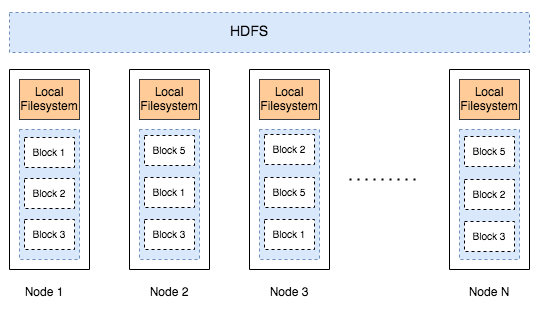
\includegraphics[width=\textwidth]{HDFSoverview}
	\centering
\end{figure}

\subsection{HDFS}\label{HDFS}
Hadoop Distributed File System, which stands for HDFS, is developed with inspiration from the guidelines described in a whitepaper about Google's Filesystem (GFS), a distributed storage paradigm to handle petabytes and larger-scale data volumes within a cluster robust to machine failures, published in 2003 \cite{ghemawat_google_2003}. 

Significant data volumes are chunked and stored within 128 MB blocks, and each block is replicated to different nodes by a factor of 3, these values are the defaults and can be changed. When the data file is requested, related blocks are constructed from the nodes across the cluster. The redundancy of the blocks guarantees availability; if one or more nodes become out of service, requested data blocks are gathered from the available redundant copies stored on other nodes. 

HDFS is a co-existing file system on the nodes it is installed, it provides a global distributed view to the files across the cluster, thus listing an HDFS directory is possible from within all nodes, the files on HDFS are listed as they exist on a local filesystem, but the physical parts of the files reside on other physical locations. 

Figure \ref{fig:HDFSoverview} depicts an overview of HDFS. The architecture of HDFS comprises Namenode, a dedicated machine to keep track of the files and folders and respective metadata like block locations across the cluster, and many data nodes on which the data blocks are residing \cite{white_hadoop_2015}. Namenode is a single-point-of-failure, meaning if the namenode is down, the whole Hadoop system is down. 

To overcome this issue, starting with version 2, Hadoop matured to a High Availability configuration depicted in Figure \ref{fig:HadoopHA} where there exist two namenodes, one active namenode, and one standby namenode communicating with the data nodes and storing edit logs in a shared folder. As the naming refers, the active namenode is in charge, whereas the standby node behaves more like a shadow system. Whenever the active namenode breaks down, the standby namenode gets activated, resulting in no service breakage for the end-user.

\begin{figure}[h!]
	\caption{Hadoop High Availability}
	\label{fig:HadoopHA}
	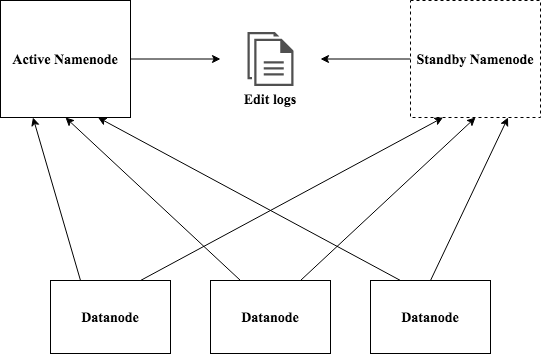
\includegraphics[width=0.7\textwidth]{HadoopHA}
	\centering
\end{figure}

\subsection{MapReduce}\label{MapReduce}
Similar to HDFS, Hadoop's MapReduce is the open-source implementation of the MapReduce framework described in a paper \cite{dean_mapreduce_2004} published in 2004. An MR flow, as depicted in Figure \ref{fig:MapReduce}, starts with assigning blocks from HDFS as input splits to mappers, computed intermediate results are then shuffled and passed to reducers where outputs are sent back to the client. Nodes running mappers and reducers provide parallel processing, scaled by simply adding new commodity computers. 

The computation is made on nodes where related data blocks reside, which explains the term data locality; executing the computation by leveraging local resources of the node where the respective data block is also stored eliminates the need for moving data across nodes for computation.

\begin{figure}[h!]
	\caption{MapReduce execution (Adapted from \cite{schatzle_giant_nodate})}
	\label{fig:MapReduce}
	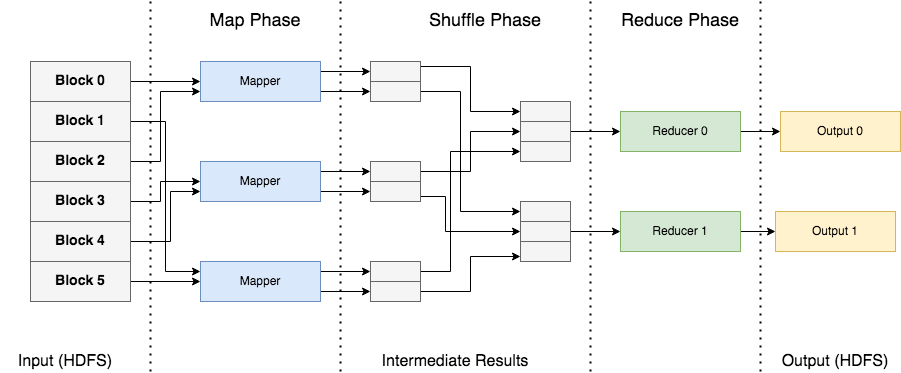
\includegraphics[width=\textwidth]{MapReduce}
	\centering
\end{figure}

\subsection{YARN}\label{YARN}
Hadoop version 2.x includes significant architectural improvements in terms of resource management. Version 1.x of Hadoop suffered shortcomings due to an overload of its resource management duties, which was handled within MRv1, where job tracker node and task tracker nodes were running the organizational load of MapReduce executions. YARN standing for "Yet Another Resource Negotiator", emerged as an intermediate layer between HDFS and MapReduce by taking over some of the load that was previously carried out by MRv1, has become a gate to batch, stream, interactive, and graph processing engines to leverage HDFS file system (Figure \ref{fig:YARNoverview}). 

After YARN, MRv1 has become MRv2 isolated from resource managerial duties regarding the previous version hence more efficient with processing oriented focus. YARN innovates Hadoop by bringing the architectural elements resource manager, which is one node dedicated to tracking resources across the cluster by availability, and node managers who reside inside each worker node and monitor the containers.

\begin{figure}[h!]
	\caption{YARN (Adapted from  \cite{dean_mapreduce_2004})}
	\label{fig:YARNoverview}
	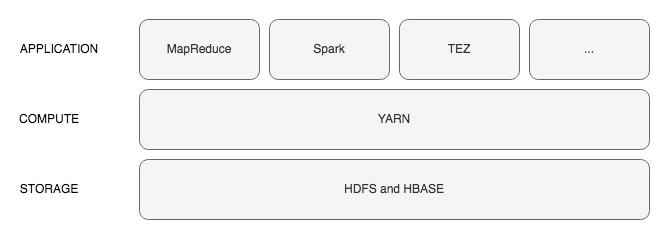
\includegraphics[width=\textwidth]{YARNoverview}
	\centering
\end{figure}


\subsection{Google Cloud Dataproc}\label{GCP_Dataproc}
Google's managed Spark and Hadoop solution, namely Dataproc \cite{noauthor_dataproc_nodate}, is a pre-configured Hadoop on PaaS service built upon pre-installed VM instances on Compute Engine \cite{noauthor_compute_nodate}, which is another service of GCP. An OS spectrum comprising Debian and\textbackslash{or} ubuntu was offered at the study's date, which are proposed as pre-installed images during the Dataproc installation process. 

While Hadoop core elements HDFS, YARN, and MapReduce reside as default frameworks, a variety of elements belonging to the Hadoop ecosystem are offered. The end-user is also offered to leverage Cloud Storage \cite{noauthor_cloud_nodate}, Google's proprietary cloud storage service, to keep data in the long term where the Dataproc cluster is meant to be terminated after usage. Utilizing Web UI or local CLI via API, the end-user can access the Dataproc cluster and single VM instances within Compute Engine. Google offers a large number of data centers around the globe.

%\paragraph{Azure HDInsight \cite{noauthor_azure_nodate}}
\subsection{Azure HDInsight}\label{Azure_HDInsight}
Azure's solution to managed Hadoop and Spark platform, HDInsight \cite{noauthor_azure_nodate} is a product of the collaboration with Hortonworks bringing Hortonworks Data Platform (HDP) to a cloud platform \cite{noauthor_azuravail_nodate}. As being so, HDInsight differs in architecture to its conjugates by not being a Hadoop cluster installed on the cloud VM service layer, namely Azure Virtual Machines; instead, it is an HDP platform optimized for the cloud. 

Another difference is that HDInsight obligates WASB, the Azure blob system, as the storage system, including an option to leverage Data Lake Storage, excluding Hadoop's native file system HDFS from the options. At the study's date, Azure was obligating Hadoop to use in High Availability mode with two master nodes but leaving hardware selection to the end-user.

\subsection{Alibaba Cloud e-MapReduce}\label{Alibaba_eMapReduce}
Alibaba Cloud's managed Hadoop service e-MapReduce \cite{noauthor_what_nodate} leveraging Apache Hadoop and Apache Spark is placed as a service layer on its Elastic Compute Service (ECS) \cite{noauthor_alielastic_nodate}, a similar approach to the one of GCP's. Even though Alibaba's number of provided data center locations beyond Mainland China are not as numerous as its conjugates, competitive regions do exist in the United States, Europe, Middle East, and the Asia Pacific. Alibaba Cloud's managed service distinct in its pre-installed Operating System, Aliyun Linux 2, a Linux distribution based on CentOS, the open-source version of RedHat Linux, developed by Alibaba Cloud. 

AliyunOS proclaims to provide a stable and reliable environment optimized for the Alibaba Cloud infrastructure and be open source at its GitHub repository \cite{noauthor_alibaba_nodate}. e-MapReduce offers a wide scale of machine types with different specifications for specific purposes like CPU intensive or memory-intensive tasks. As with GCP, on Alibaba Cloud e-MapReduce, the type of storage, whether it shall be HDFS or leverage Object Storage Service (OSS) \cite{noauthor_oss_nodate}, Alibaba's cloud storage, can be specified by the end-user.

\subsection{HiBench Benchmark Suite}\label{benchmarks_hibench}
The open-source HiBench \cite{noauthor_intel-bigdatahibench_2021} implementation, introduced to the community in 2010 \cite{huang_hibench_2010}, is motivated by the aim of providing a comprehensive and representative benchmark for Hadoop, helping evaluate different big data frameworks in terms of speed, throughput, and system utilization. At the study's date, the current version of HiBench is 7.1, comprising 29 benchmarks categorized in 6 sections (Micro, Machine Learning, SQL, Websearch, Graph, and Streaming). Table \ref{tab:hibench-wrkl} lists the Hadoop related workloads in HiBench 7.1 \cite{noauthor_release_nodate}. 

The benchmarks in the category Micro are taken from Hadoop's native benchmark tools, where Dfsioe is the enhanced version of its originator Dfsio, calculating the average I/O rate, averaging throughput of each map task, and aggregating throughput of the cluster. The column "Engine" points out HiBench's dependencies, which are downloaded when Apache Maven compiles the benchmark suite, and leveraged during benchmark executions; Hive engine is leveraged to run HiveQL queries for Scan, Join, and Aggregation benchmarks. The Hadoop based ML benchmarks are driven by Mahout; Nutch Engine is leveraged for Nutchindexing benchmark; Pegasus, a peta-scale graph mining system, calculates PageRank algorithm. The dependencies execute benchmark tasks by translating respective jobs into MapReduce. HiBench's predefined default data scales -- namely, tiny, small, large, huge, gigantic, and bigdata -- provide a scale varying from 32 KB up to 300 GB for Sort, 6 GB for Terasort, and 1.6 TB for Wordcount. User-defined data scales are also applicable within HiBench configurations.


\begin{table}
	\centering
	\small
	\caption{HiBench 7.1 - Hadoop-related Workloads}
	\label{tab:hibench-wrkl}
	\begin{tabular}[b]{ p{3.0cm} p{3.0cm} p{3.0cm} }
		\hline
		\textbf{Category} & \textbf{Workload} & \textbf{Engine} \\
		\hline
		\multirow{4} {3cm} {Micro} & Sort & \multirow{4} {3cm} {M/R} \\
		 & Terasort &  \\
		 & Wordcount & \\
		 & Dfsioe & \\
		\hline
		\multirow{3}{3cm}{SQL} & Scan & \multirow{3} {3cm} {Hive} \\
		 & Join & \\
		 & Aggregation & \\
		\hline
		\multirow{2}{3cm}{ML} & Bayes & \multirow{2} {3cm} {Mahout} \\
		 & Kmeans &  \\
		\hline
		\multirow{2}{3cm}{Websearch} & Nutchindexing & Nutch Engine \\
		 & Pagerank & Pegasus \\
		\hline
	\end{tabular}
\end{table}

%Serkan: Related work kısmında referans sayısı biraz az olmuş. Daha kısa kısa başka alanlarda yapılmış benchmarklara da değinip genişletmek gerekir. Ben de biraz araştırma yapıp eklemeler yapacağım, siz de yaparsınız.
\section{Related Work}
Our search for related work to the study, which focuses on benchmarking Hadoop on PaaS, i.e., managed Hadoop systems, yielded papers with similar approach to our intention, and are referred to first and second below. Other works we have found present differing approaches in benchmarking, such as leveraging multiple benchmark suites on the same cluster, stressing Hadoop on IaaS with manually installed clusters, testing the before and after tweak performances, comparing different Hadoop environments, or comparing Hadoop vs. Spark frameworks.

Poggi et al. \cite{poggi_characterizing_2018} conducted a comprehensive study benchmarking Hadoop PaaS services provided by Amazon (EMR), Google (Dataproc), and Azure (HDInsight). The benchmark tool they used, namely BigBench (TPCx-BB), is an industry-standard benchmarking framework developed by Transaction Processing Performance Council (TPC). TPCx-BB comprises 30 business use cases and differentiates from SQL-only benchmarks by also requiring other frameworks like MapReduce, user code (UDF), Natural Language Processing, and Machine Learning. The researchers' study objective was twofold: Firstly, it was characterizing BigBench queries and out-of-the-box performances of Hive and Spark in the cloud, and secondly, it compared the cloud vendors in terms of reliability within a data scale ranging from 1GB to 10TB. The medium-size clusters put under test consist of 16 cores and 60+GB memory for the master node and 16 data nodes with 128 total cores. The executions of TCPx-BB along with the data scales showed that Hive performs in most cases better in up to 1TB, whereas, in a 10TB data scale, Spark hits a significantly better performance, up to two times faster than Hive.

%Emre: EKLENEN (poggi_state_2016)
In \cite{poggi_state_2016}, Poggi et al. surveyed entry level Hadoop PaaS offerings, namely, Google Cloud Dataproc, Amazon EMR, Azure HDInsight, and Rackspace Cloud Big Data within the time space March-July 2016. A local Hadoop cluster was also benchmarked as a criterion setup for comparing the impact of fine-tuning the software stack. Hive was selected as benchmark subject for SQL-on-Hadoop services of the providers, leveraging TPC-H decision support benchmark, where respective cost\textbackslash{}performance rates and scalability in data and computation was considered as well. The study pointed out that the dynamic upgrade capabilities of provider services delivered even better performance after daily based service updates; the pricing varied even with very similar hardware and software specs due to the pricing policies of respective providers.

%Emre: EKLENEN (wang_improved_2020)
Wang et al. \cite{wang_improved_2020} leveraged HiBench to test the effect of their optimization solution on Hadoop's MapReduce framework. The problem definition was targeting the insufficiency of the current MapReduce framework for efficiently handling intermediate data; the output of maps was physically stored on the disk and also read from there to got passed to the reduce slots; as the number of mappers and reducers increase, expensive disk seeks occur resulted in high execution times. The researchers' proposal, APA (Aggregation, Partition, and Allocation), aggregated intermediate data in each rack to one file and a file host pushes the data to reduce tasks. Benchmarking the experimental setup consisting of 50 data nodes across 10 racks and 40 Gbps rack interconnectivity yielded 40\% to 50\% performance improvement. 

%Emre: EKLENEN {hwang_cloud_2016} 
Hwang et al. \cite{hwang_cloud_2016} used HiBench and four other benchmarks (YCSB, CloudSuite, BenchClouds, and TPC-W) on Amazon EC2 instances introducing new performance metrics applicable to IaaS, PaaS, SaaS, and hybrid clouds. Argued and tested were the cloud scaling strategies vertical scaling (scale-up), horizontal scaling (scale-out), and mixed approach. The researchers conducted the aforementioned benchmarks on cluster scale strategies. The study has drawn multiple conclusions proposing new performance metrics, differentiating between scaling-up and scaling-out strategies and applicable use cases, the performance of scale-out vs. cost-effectiveness of scale-up approaches, and the close relation between cloud productivity and system elasticity, efficiency, and scalability.

Ahn et al. \cite{ahn_performance_2018} put Spark on YARN's performance on the test with HiBench to hande a deluge of data generated by IoT devices. The experiment was run on a cluster with one master and three worker nodes, each node possessing an Intel® Xeon® processor with 20 cores and 128GB main memory meaning 60 cores and 384GB memory in total. HiBench workloads Micro (comprising Sort, TeraSort, and Wordcount), SQL (comprising Aggregation, Join, and Scan), and Machine Learning (comprising Bayes, Logistic Regression, Gradient Boosting Tree, Random Forest, and Linear Regression) was leveraged by a chosen data scale of 30 GB. Spark occupied memory during the whole job execution, which reduces I/Os' negative impact on processor performance. The conductors modified YARN's minimum memory allocation and Spark executor settings to optimize resource usage so that the Spark executors' overall loads remained below total system memory. Alongside with HiBench's duration and throughput report, CPU / memory utilization and disk throughput were profiled as well. This paper's finding pointed out that Spark guarantees performance when provided with enough memory.

Han et al. \cite{han_impact_2017} studied the impact of memory size on big data processing through Hadoop and Spark performance comparison leveraging HiBench's k-Means workload as the only benchmark. For memory sizes 4, 8, and 12 GB, across a data scale from 1 to 8 GB, k-Means benchmark for Hadoop and Spark was executed. The results depicted Spark's overperforming Hadoop unless the total input data size was smaller than 33.5\% of worker nodes' total memory size. After reaching that ratio, Spark suffered from insufficient memory resources and led to interoperate with HDFS causing a sharp decrease in its performance and brings Hadoop in throughput and duration performance to the front. The conductors conducted a second experiment to determine if Spark's performance can be improved by tweaking the allocation setting for storage memory and shuffle memory while remaining within the specified memory limitations of 4, 8, and 12 GB. Executing HiBench's k-means benchmark outputs a report interpreted by the conductors as Spark show a 5-10\% and 15\% maximum improvement in processing time.

Ivanov et al. \cite{ivanov_performance_2015} compared the performances of two enterprise-grade applications, DataStax Enterprise (DSE), a production-level implementation of Apache Cassandra with extended features like in-memory computing and advanced security, to name but two, and Cloudera's Distribution of Hadoop (CDH) comprising core Hadoop elements HDFS and YARN integrated with elements belonging to the Hadoop ecosystem. DSE's HDFS compatible file system CSF lets Hadoop applications run without any modification. The conductors installed the latest stable releases of both software on equal CPU, memory, and network infrastructure configuration; for both installations, default system parameters have been left with their defaults. HiBench's three chosen workloads (CPU-bound wordcount, I/O-bound dfsioe, and mixed HiveBench) were executed three times; furthermore, the average values have been taken for representativeness. Their study's conclusions proclaimed linear scaling of both systems by increasing data size, while CDH outperformed DSE in read-intensive workloads, DSE performed better in write-intensive workloads. Leveraging HiBench was where the study differed from other studies using the YCSB benchmark suite. HiBench's results confirmed the latter's output as well.

Samadi et al. \cite{samadi_performance_2018} conducted an experimental comparison between Spark and Hadoop installed on virtual machines on Amazon EC2 by leveraging nine among the provided HiBench workloads. Accuracy reasons led the conductors to run the workloads three times, concluding input data scales of 1, 3, and 5 GB, respectively. Based on the outputs comprising duration, throughput, speed up, and CPU/memory consumption, the conclusion has drawn Spark consuming less CPU and performing better on all workload results over Hadoop. 

\section{Materials and Methods}
In the study, we benchmarked Hadoop on PaaS services of three different CSPs in terms of comparing their performances accompanied by respective resource utilization across the worker nodes: GCP Dataproc, Azure HDInsight, and Alibaba Cloud e-MapReduce, each recognized in Gartner's 2020 Magic Quadrant for Cloud Infrastructure and Platform Services \cite{noauthor_gartner_nodate} either in leading or in niche section.

We constructed the benchmark study in two use cases: Use Case 1 aims to map the overall performance behaviors of respective CSP's service within HiBench's predefined data scales, huge and gigantic. The following benchmarks have been executed on the clusters of the respective providers: Micro (Sort, Terasort, Wordcount, and Dfsioe), SQL (Scan, Join, and Aggregation), ML (Bayes and Kmeans), and Websearch (Pagerank).

In Use Case 2, we selected one I/O intensive benchmark task (Sort) and one CPU intensive benchmark task (Wordcount). Subsequently, the scalability of these benchmark tasks was evaluated using increasing data sizes generated by HiBench: Tiny, Small, Large, Huge, and Gigantic. The largest predefined HiBench data scale, namely Bigdata, would cross the installed clusters' storage limits. Hence, it was omitted in the benchmark evaluations.

Bound by the availability of their respective hardware and software options, we selected the same or close settings within providers' promises. Concerning our aim to benchmark managed systems as they come out-of-the-box, we put three basic principles to stick with for each provider in order to align initial circumstances before benchmark execution: Among the CSPs, the respective data center's geographic location shall be the same or close (1), processor number and memory capacity (by providers' promise) shall be same or as close as possible (2), and selected Hadoop versions among the providers' offerings shall be close to each other and remain within version limits supported by HiBench 7.1 (3). 

Thus Frankfurt is selected as the location for all providers' data centers; within the given options, we selected 8 CPUs/64GB RAM for the master node and 4 CPUs/32 GB RAM for each worker node totaling 12 CPUs and 96 GB worker compute power for the cluster; within proposed images, Hadoop versions 2.7.3, 2.8.5, and 2.9 have been selected. Specified cluster installation options and details are given in Table \ref{tab:csp-configs}.

Without applying any performance tweak operation to the respective configurations, we immediately executed several Hadoop benchmarks from HiBench's Micro, SQL, ML, and Websearch categories. We only modified the default cluster's configuration in cases where the benchmark was detained from running, reported in the Discussion section.

By leveraging a low-footprint bash script based on sar commands, we collected system utilization records addressing CPU, Memory, and I/O behavior on each worker node of the cluster during the benchmark execution. The captured data enabled us to visualize the system utilization on each worker node within the cluster over the respective benchmark's execution time. To provide data locality, if a specific data block to process does not reside on the same node where there is an available map slot, YARN transfers the respective block to the node with a free slot requiring a network activity, a possible decreasing impact over the performance. 

However, due to the small cluster size consisting of 3 nodes, we excluded the network activity track with the assumption that data locality during the benchmark's executions is either provided, or data blocks moved within rack locality is likely to have the least impact on the performance.

\begin{table}
	\centering
	\small
	\caption{Selected configurations on CSPs' managed Hadoop services}
	\label{tab:csp-configs}
	\begin{tabular}[h!]{ p{2.0cm} p{2.3cm} p{3.3cm} p{2.6cm}  }
		\hline
		{} & \textbf{GCP} & \textbf{Azure} & \textbf{Alibaba Cloud}\\
		\hline
		Service & Dataproc & HDInsight & e-MapReduce \\
		Region & europe-west3-a & Germany West Central & eu-central-1 \\
		Location & Frankfurt & Frankfurt & Frankfurt \\
		Image & 1.4-ubuntu18  & HDI 3.6 & EMR-3.32.0 \\
		OS & ubuntu18.04 & ubuntu 16.04 & Aliyun Linux 2 \\
		Hadoop v. & 2.9 & 2.7.3 & 2.8.5 \\
		Java & 1.8.0\_275 & 1.8.0\_275 & 1.8.0\_252 \\
		\hline
		\multicolumn{4}{ c }{MASTER NODE} \\
		\hline
		Machine Type & e2-highmem-8 & A8m v2 & ecs.se1.2xlarge \\
		Processors & 8 vCPU & 8 cores & 8 vCPU \\
		Memory & 64 GB RAM & 64 GB RAM & 64 GB RAM \\
		Extras & -- & 1 Master Node clone for HA, 3 extra nodes for Zookeeper & -- \\
		\hline
		\multicolumn{4}{ c }{WORKER NODES} \\
		\hline
		\# of Nodes & 3 & 3 & 3 \\
		Machine Type & e2-highmem-4 & A4m v2 & ecs.se1.xlarge \\
		Processors & 4 vCPU & 4 cores & 4 vCPU \\	
		Memory & 32 GB RAM & 32 GB RAM & 32 GB RAM \\	
		Storage & HDFS 1000 GB & \multirow{3}{ 8em }{WASB \\
			\textit{Azure blob storage}} & HDFS 1000 GB \\	
		Replication & 2 &  & 2 \\	
		Block size & 128 MB &  & 128 MB \\
		\hline
	\end{tabular}
\end{table}

%Serkan: Results tek başına çok uzun bir section olduğu için takip etmesi zor oluyor. O yüzden her use case'i  ayrı bir sectiona böldüm. Evaluation setup hakkındaki kısmı da subsection olarak  Materials and Methods kısmının altına taşıdım.

\subsection{Evaluation Setup}
HiBench's Hadoop related benchmarks in the categories Micro (Sort, Terasort, Dfsioe, and Wordcount), SQL (Scan, Join, and Aggregation), ML (Bayes and Kmeans), and Websearch (Pagerank) have been executed on all three CSPs' managed Hadoop services. 

During benchmark runtime, resource utilization on worker nodes has been captured. The plots are organized as follows: Top-left, top-right, and bottom-left plots represent CPU (\%user for Azure and Alibaba, \%nice for GCP since M/R jobs are nice'd on GCP), memory (\%memused), and I/O utilization (read transfers and write transfers per second) on each worker node of the respective cluster over time. CPU utilization lines are given in blue tones; memory utilization lines are given in fuchsia tones, I/O-read and I/O-write tps' represented with orange tones and green tones. Even though the coloring convention might sound confusing, it gives a clear portrait of the entire benchmark process's utilization behavior over time. The left-hand side x-axis measures CPU/Memory usage in percent; the right-hand side x-axis measures I/O-read and I/O-write transfers per second. 

The bottom-right plot represents the comparative benchmark performance outputs of the respective CSPs. Duration measure in seconds is expected to be perceived as "the lower is the better". On contrary, throughput is the amount of processed data per second in bytes. Thus, the higher values of throughput indicate better performance results.

For each use case, we provided spider charts, i.e., radar plots, to give a comparative overview for system utilization vs. benchmark performances of relevant CSPs. In these plots, normalized average values of the captured CPU, Memory, and I/O data on the worker nodes have been averaged a second time in order to get scalar CPU, Memory, and I/O values representing the cluster's average performance. 

For the sake of better visualization of I/O utilization, we removed 0 valued instances before taking the I/O-read and I/O-write data average. Combining the values mentioned above with normalized duration and throughput report values of HiBench outputs the study's spider plots. Nevertheless, for the spider plots, both throughput and duration shall be perceived as "higher is better". Even though the duration is lower-is-better, for the sake of proper visualization, we display the shortest duration as the largest value, making it the most visible on the plot. 


%Serkan: Use case'leri ayırdıktan sonra bir kısa giriş yapıp sonuçlara genel bakış verip daha sonra detaylı açıklamalar gelecek şekilde organize ettim. Genelden detaya ilerleme okuma sürecinde daha kolay oluyor. 

\section{Use Case 1 Results}

In the Use Case 1 evaluations, we assessed the performances of CSP's services using HiBench's benchmark tasks with predefined data scales huge and gigantic, separately. More specifically, HiBench's benchmark tasks of Micro (Sort, Terasort, Wordcount, and Dfsioe), SQL (Scan, Join, and Aggregation), ML (Bayes and Kmeans), and Websearch (Pagerank) were executed on the respective clusters of each Cloud Service Provider. 

The overall HiBench results for the use case is shown in Table \ref{tab:uc1-results}. A summarized version of the benchmark results related to system utilization averages of respective CSPs are illustrated in Figure \ref{fig:uc1-huge-new} and Figure  \ref{fig:uc1-gigantic-new}. The spider plots also depict the main character of the respective benchmark, whether it is I/O-bound like in Sort or CPU-bound as in Wordcount, or both, distributed in the map and reduce phases as in SQL benchmarks Scan, Join, and Aggregation. In most cases, the systems that can afford more utilization appeared to have relatively better performance.


%%Use Case 1 benchmark results:
\begin{table}
	\centering
	\small
	\caption{Use Case 1 benchmark results }
	\label{tab:uc1-results}
	\begin{tabular}[b]{ l r r r r r r r }
		\multicolumn{8}{ l }{Data Scale: Huge} \\
		{} & {} & \multicolumn{2}{ c }{\textbf{Dataproc}} & \multicolumn{2}{ c }{\textbf{HDInsight}} & \multicolumn{2}{ c }{\textbf{e-MapReduce}} \\
		\hline
		{Benchmark} & {IDS} & \begin{math}D_{(s)}\end{math} & \begin{math}T_{(MB/s)}\end{math} & \begin{math}D_{(s)}\end{math} & \begin{math}T_{(MB/s)}\end{math} & \begin{math}D_{(s)}\end{math} & \begin{math}{T_{(MB/s)}}\end{math} \\
		\hline
		Sort & 3.28 & 70 & 47.11 & 131 & 25.08 & 111 & 29.42 \\
		Terasort & 32.00 & 667 & 47.99 & 858 & 37.28 & 1054 & 30.37 \\
		Wordcount & 32.85 & 978 & 33.60 & 1470 & 22.34 & 889 & 36.95 \\
		Dfsioe-r & 26.99 & 294 & 91.77 & 662 & 40.79 & 245 & 110.21 \\
		Dfsioe-w & 27.16 & 379 & 71.73 & 658 & 41.30 & 281 & 96.49 \\
		Scan & 2.01 & 73 & 27.63 & 157 & 12.83 & 74 (*) & 27.19 (*) \\
		Join & 1.92 & 181 & 10.61 & 356 & 5.39 & 175 (*) & 10.95 (*) \\
		Aggregation & 0.37 & 97 & 3.86 & 215 & 1.73 & 97 (*) & 3.85 (*) \\
		Bayes & 1.88 & 2604 & 0.72 & 6120 & 0.31 & 3017 & 0.62 \\
		Kmeans & 20.08 & 2321 & 8.65 & 2313 & 8.68 & 2070 & 9.70 \\
		Pagerank & 2.99 & 1544 & 1.94 & 3334 & 0.90 & 2458 & 1.22 \\
		\hline
		\multicolumn{8}{ l }{Data Scale: Gigantic} \\
		{} & {} & \multicolumn{2}{ c }{\textbf{Dataproc}} & \multicolumn{2}{ c }{\textbf{HDInsight}} & \multicolumn{2}{ c }{\textbf{e-MapReduce}} \\
		\hline
		{Benchmark} & {IDS} & \begin{math}D_{(s)}\end{math} & \begin{math}T_{(MB/s)}\end{math} & \begin{math}D_{(s)}\end{math} & \begin{math}T_{(MB/s)}\end{math} & \begin{math}D_{(s)}\end{math} & \begin{math}{T_{(MB/s)}}\end{math} \\
		\hline
		Sort & 32.85 & 715 & 45.94 & 787 & 41.72 & 896 & 36.68 \\
		Terasort & 320.00 & 9821 & 32.58 & ---(**) & ---(**) & 9660 & 33.13 \\
		Wordcount & 328.49 & 10131 & 32.42 & 13596 & 24.16 & 8671 & 37.88 \\
		Dfsioe-r & 216.03 & 915 & 236.11 & 1886 & 114.54 & 660 & 327.29 \\
		Dfsioe-w & 217.33 & 1347 & 161.39 & 1914 & 113.57 & 1060 & 205.12 \\
		Scan & 20.10 & 457 & 43.96 & 514 & 39.09 & 407 (*) & 49.38 (*) \\
		Join & 19.19 & 595 & 32.27 & 761 & 25.24 & 594 (*) & 32.32 (*) \\
		Aggregation & 3.69 & 523 & 7.05 & 594 & 6.20 & 565 (*) & 6.52 (*) \\
		Bayes & 3.77 & 5350 & 0.70 & 12589 & 0.30 & 6363 & 0.60 \\
		Kmeans & 40.16 & 4541 & 8.84 & 4042 & 9.94 & 4034 & 9.96 \\
		Pagerank & 19.93 & 8371 & 2.38 & 11779 & 1.70 & 13893 & 1.43 \\
		\hline
		\multicolumn{8}{r}{IDS: Input Data Size (GB); \begin{math}D_{(s)}\end{math}: duration (sec); \begin{math}T_{(MB/s)}\end{math}: throughput (MB/sec)} \\
		\multicolumn{8}{ r }{(*) Benchmark succeeds after modifying preconfiguration, more on this in Discussion } \\
		\multicolumn{8}{ r }{(**) System failure due to insufficient space on HDFS, more on this in Discussion } \\
		\hline
	\end{tabular}
\end{table}

\begin{figure}[p]
	\caption{Use Case 1 - Overview to system utilization in data scale huge}
	\label{fig:uc1-huge-new}
	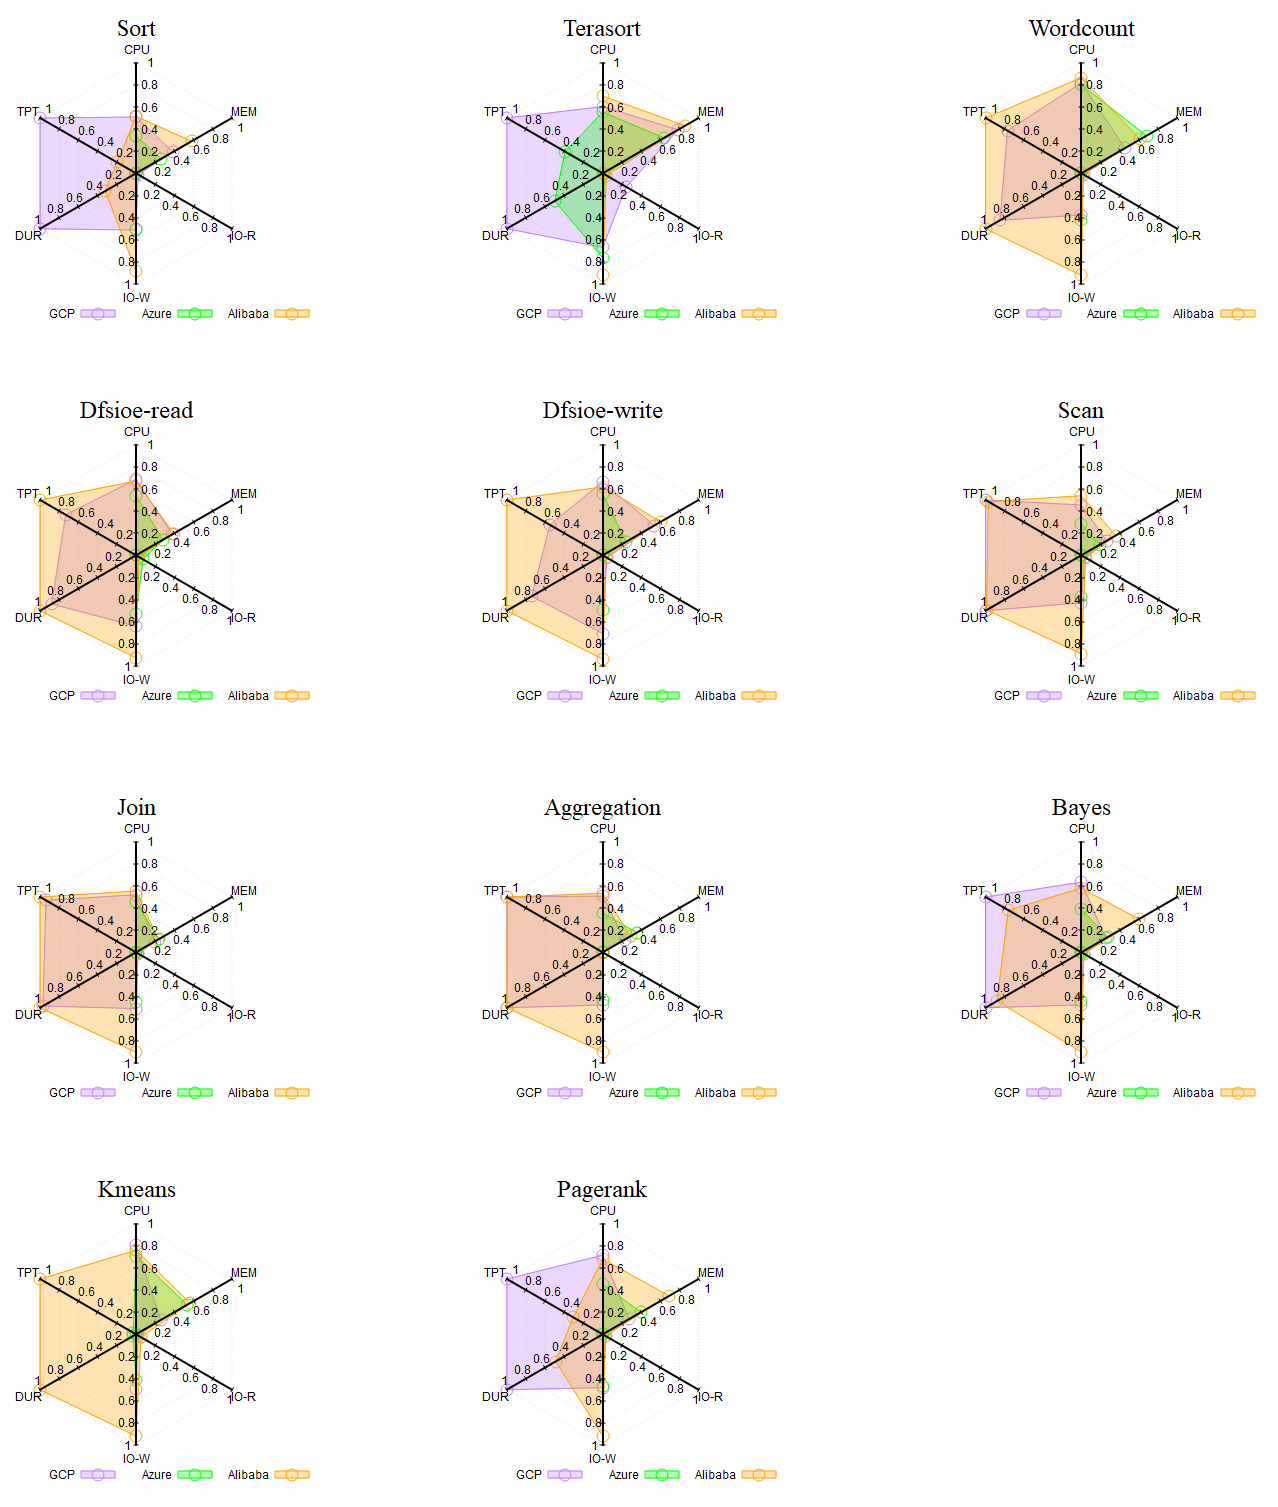
\includegraphics[width=\textwidth]{uc1-huge-new}
	\centering
\end{figure}

\begin{figure}[p]
	\caption{Use Case 1 - Overview to system utilization in data scale gigantic}
	\label{fig:uc1-gigantic-new}
	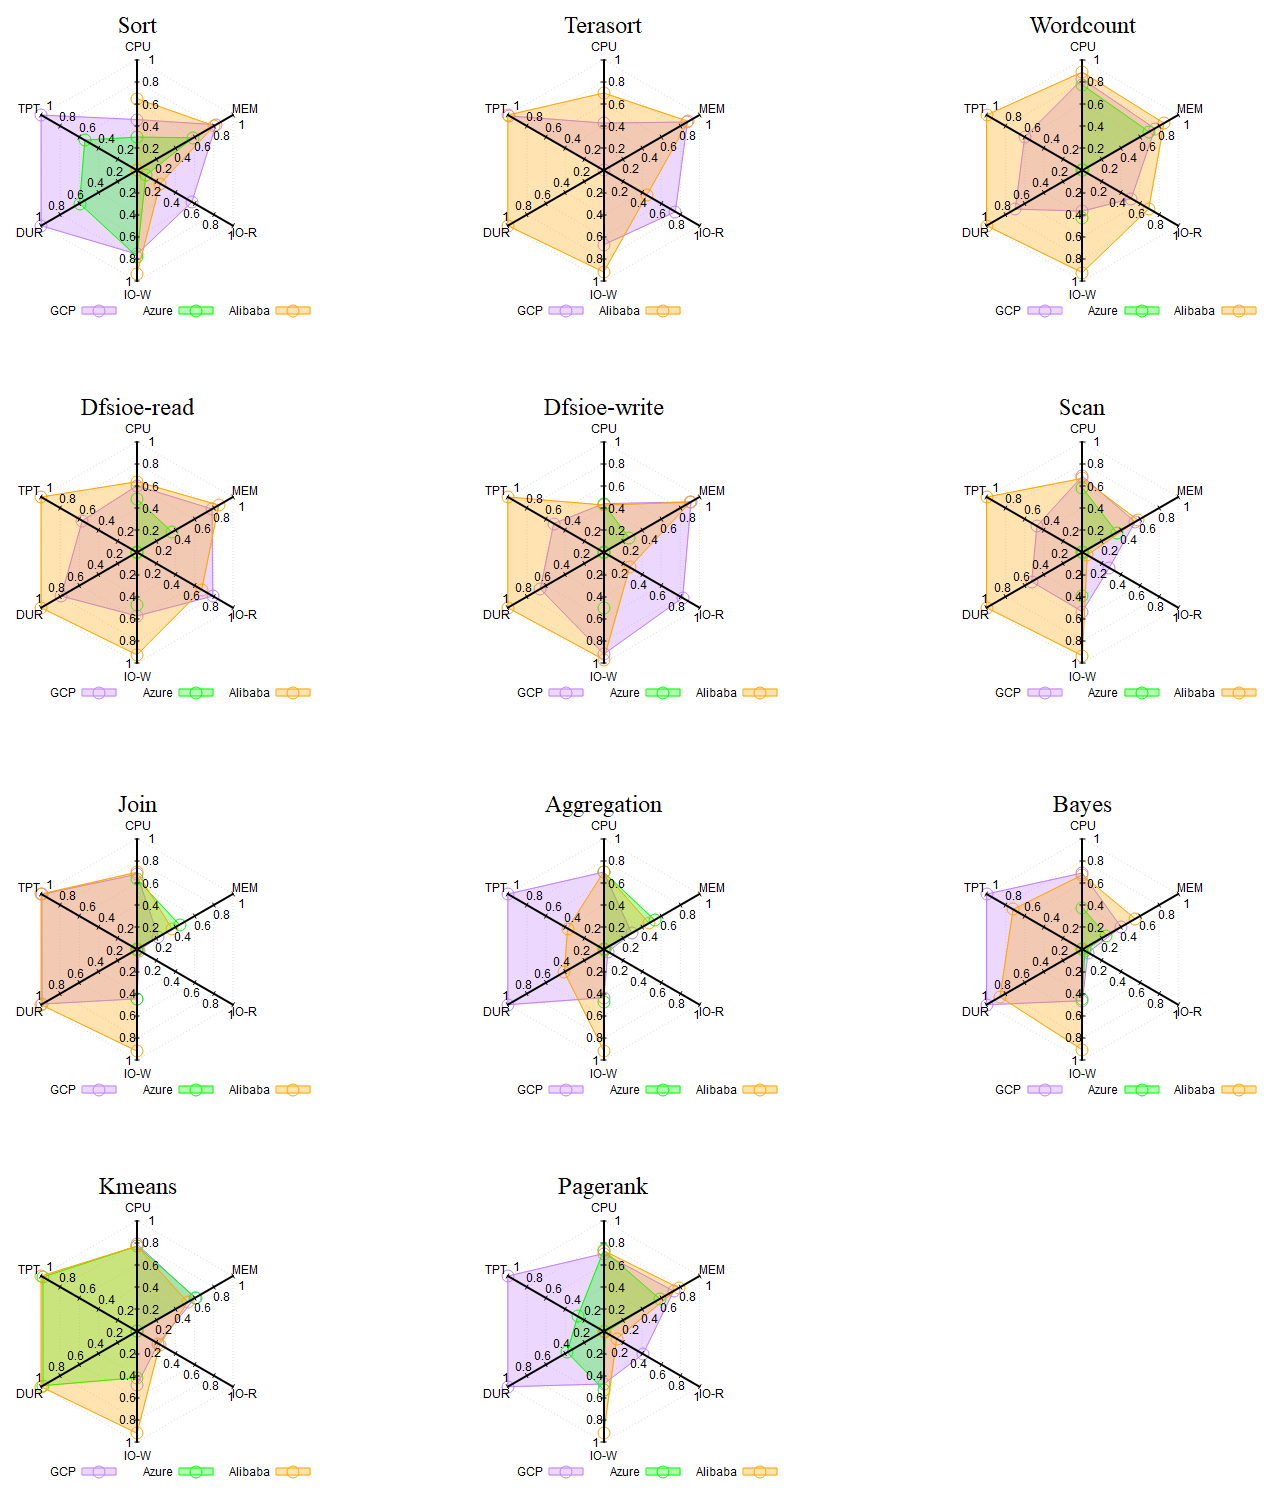
\includegraphics[width=\textwidth]{uc1-gigantic-new}
	\centering
\end{figure}


\subsection{Sort Benchmark Results}
CPU utilization in GCP and Alibaba condense around 80\% to 98\%, whereas in Azure, the range spans between 50\% and 90\% as shown in Figure \ref{fig:uc1-srt-h-cmidt}. Memory loads in GCP and Alibaba among the worker nodes display a harmonic behavior between 20\% to 40\% and 90\% to 100\%, respectively, whereas the memory load in Azure's worker nodes varies between 10\% and 50\%. In the second half of the benchmark execution, I/O write transfers in GCP and Alibaba show peaks at about 500 tps, whereas Azure I/O transfer is limited with 100 tps. GCP carrying out the highest throughput, thus reaching the shortest duration of 70 seconds.

\begin{figure}[p]
	\caption{UC1 - Sort (Huge; 3.2 GB)}
	\label{fig:uc1-srt-h-cmidt}
	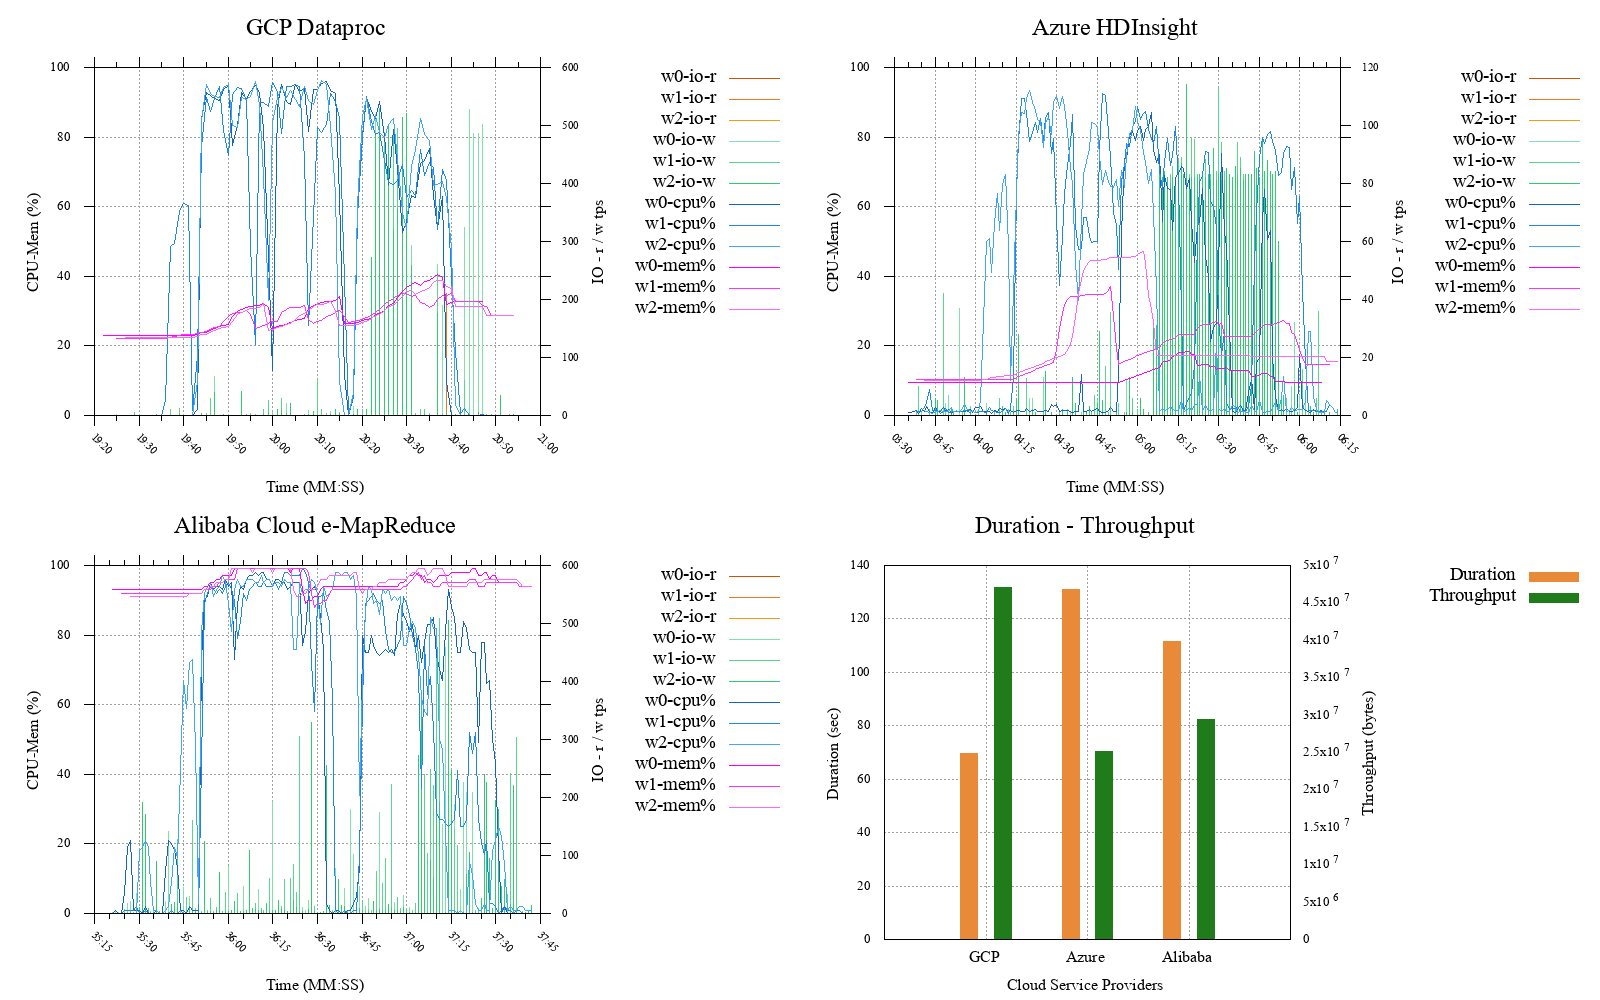
\includegraphics[width=\textwidth]{uc1-srt-h-cmidt}
	\centering
\end{figure}


Switching the data scale for Sort benchmark to gigantic, GCP's processor load condenses around 80\% - 95\% where its memory load rises to range 80\% - 100\%; I/O write transfers behave at about 500 tps where I/O reads reach 1000 tps in the second half of the benchmark process as demonstrated in Figure \ref{fig:uc1-srt-g-cmidt}. Azure's processor and memory performances depict a looser behavior not utilizing the maximum potential, whereas I/O-read and I/O-write tps' reach their maximum at 200 and 350, respectively. Alibaba's resource utilization depicts a high memory load of 90\% - 100\% dropping to 70\% and about 83\% on partial nodes in the second half. As with the processor load behaving between 80\% and 100\% in the first half dropping to about 50\% in the second half where I/O write reaches the peak at 800 tps, which results in GCP embarking highest and Azure the second highest throughput, respective durations output in 715 and 758 seconds.

\begin{figure}[p]
	\caption{UC1 - Sort (Gigantic; 32 GB)}
	\label{fig:uc1-srt-g-cmidt}
	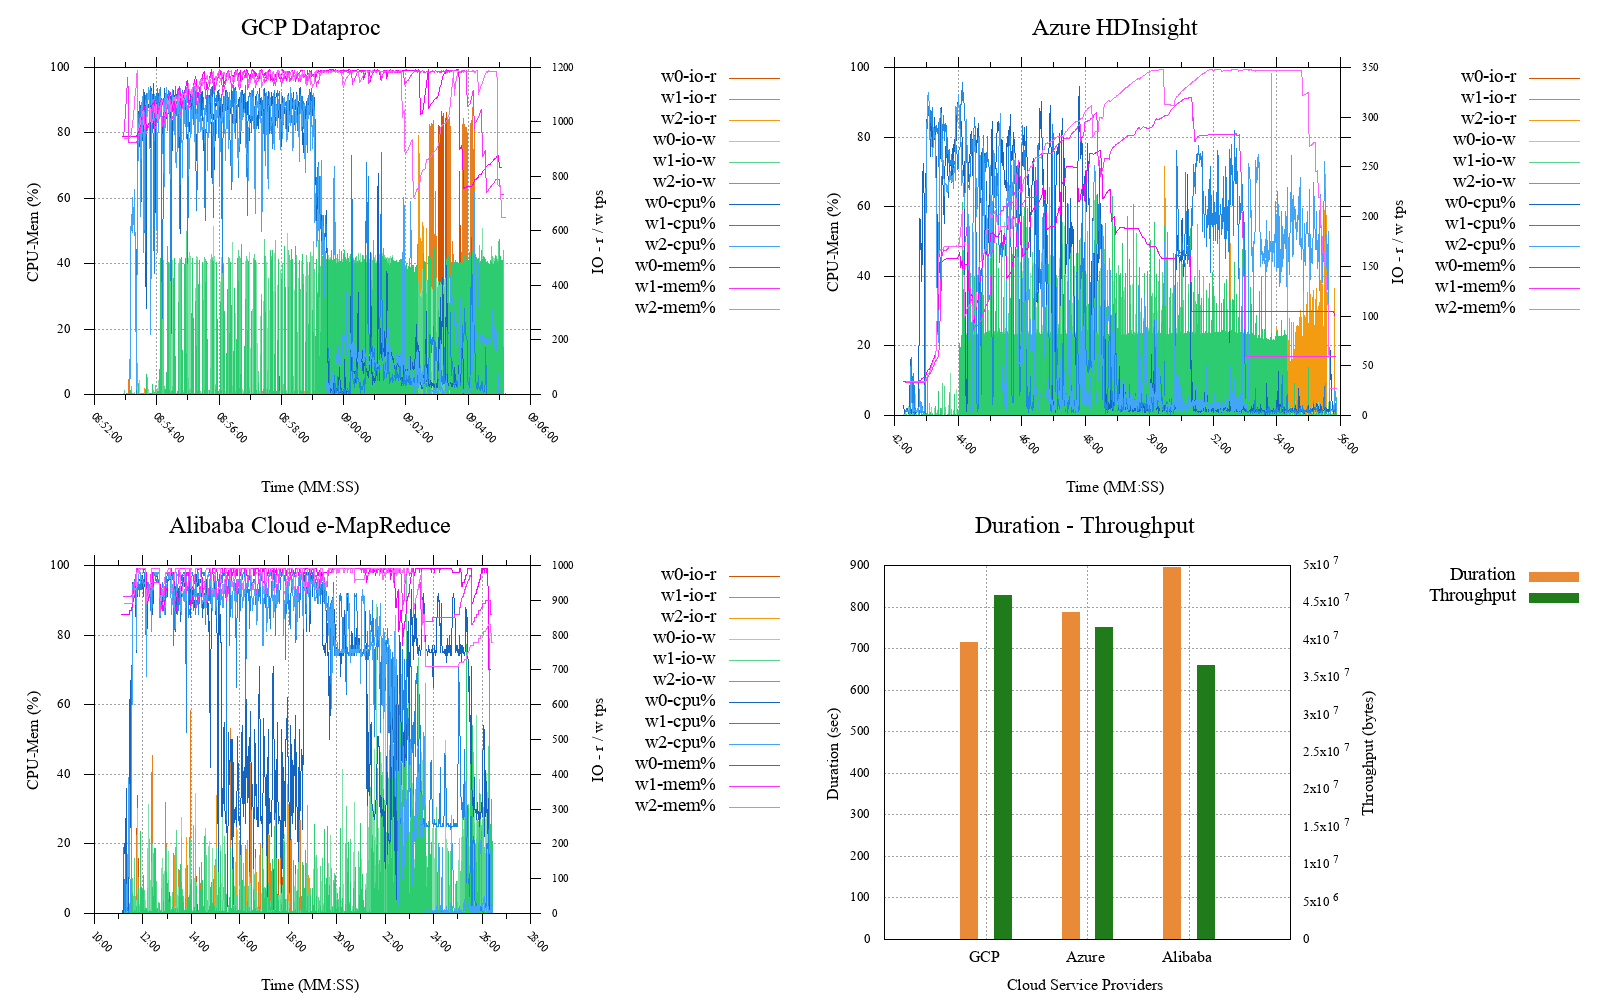
\includegraphics[width=\textwidth]{uc1-srt-g-cmidt}
	\centering
\end{figure}

\subsection{Terasort}
In the Terasort task with Huge scale dataset, GCP depicts a high utilization of processors at a range of 80\% - 100\%, memory moving from 80\% to 100\%, and I/O behavior 500 tps in overall and peaking at 1000 tps in I/O-read, resulting in the highest throughput in 667 seconds response time among other CSPs as shown in Figure \ref{fig:uc1-tera-h-cmidt}. Azure's processor and memory utilization fluctuate in overall execution where memory performance incrementally reaches 100\% in one node, a stable I/O-write in overall process at about 70 tps peaking at 250 tps reaches the second highest throughput in 858 seconds. With high memory and processor utilization and varying I/O tps' in the overall process, Alibaba falls back in embarking throughput and resulting in 1054 seconds response time.

\begin{figure}[p]
	\caption{UC1 - Terasort (Huge; 320 MB)}
	\label{fig:uc1-tera-h-cmidt}
	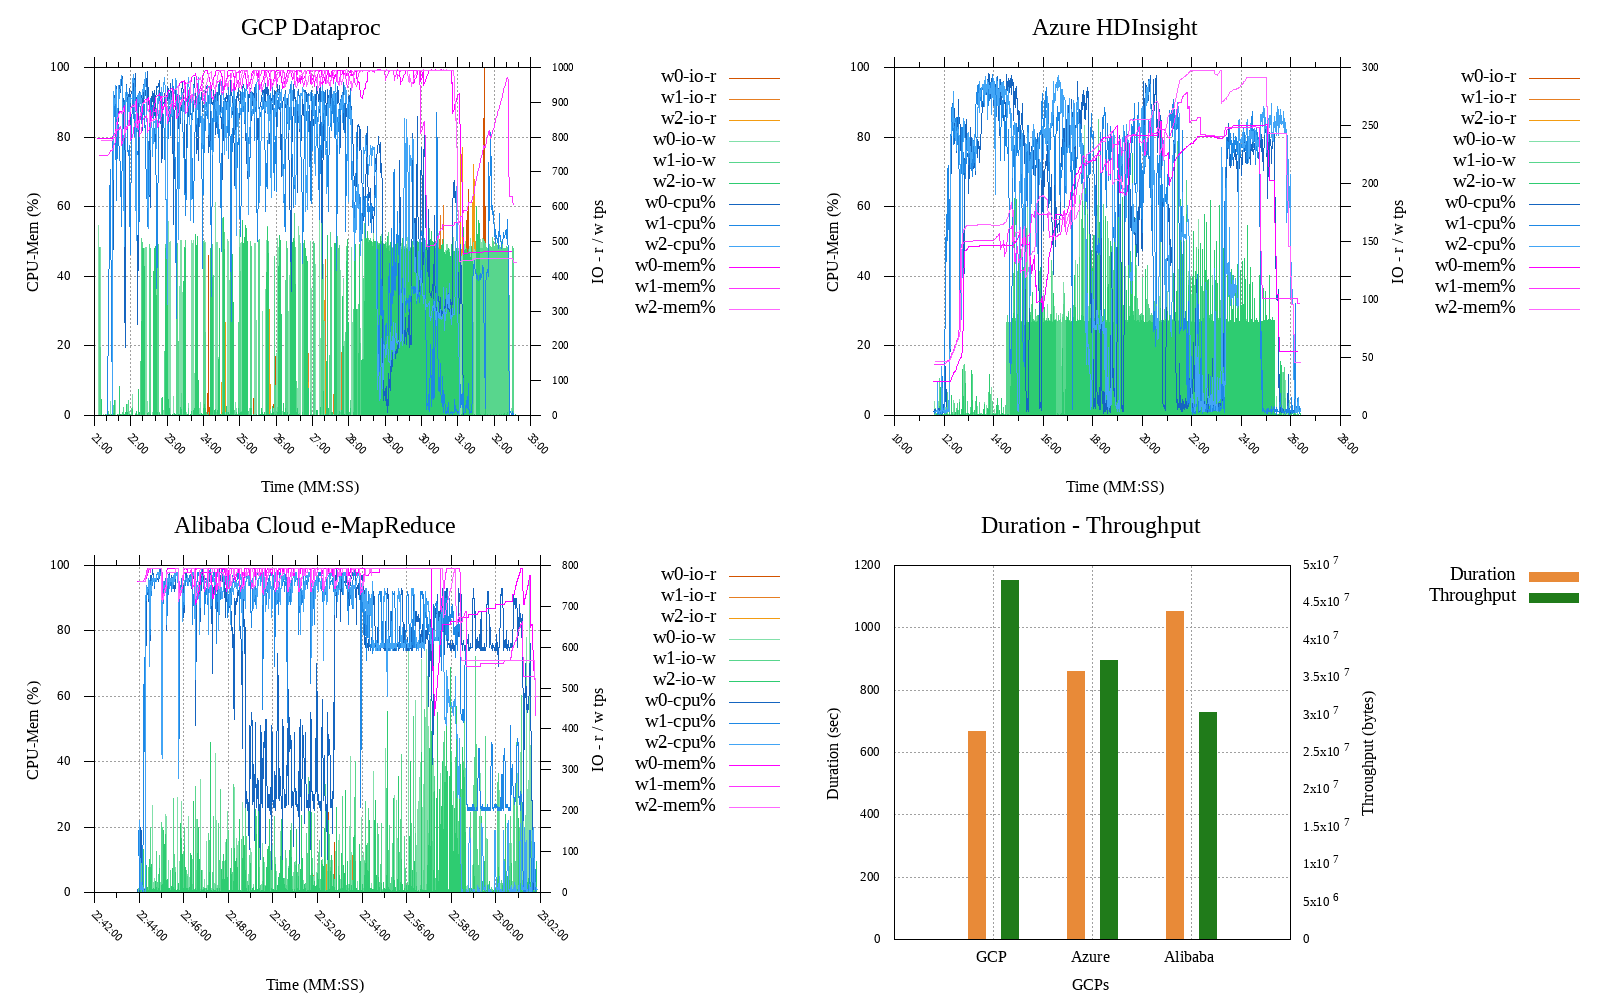
\includegraphics[width=\textwidth]{uc1-tera-h-cmidt}
	\centering
\end{figure}

When using the gigantic scale dataset, dramatic resource utilization changes were observed on all CSPs as displayed in Figure \ref{fig:uc1-tera-g-cmidt}. During all benchmark processes, GCP depicts very condensed high utilization on the processor at a broad range of 30\% to about 95\%, memory consumption between 95\% and 100\%, and I/O read transfer varying between 800 to 1100 tps . On the other hand, Azure fails to complete the benchmark on three attempts, suffering from YARN insufficient HDFS allocation requested for bringing the job further. I/O scores drop to null, and task raises failure. Alibaba Cloud's resource utilization goes within maximum levels where processor utilization depicts a consumption of 80\% to 90\% overall, memory utilization at its highest during all process, and I/O reads and writes moving along the 600 tps' and peaking around 1600 tps. With a slightly higher value in throughput, Alibaba performs best with 9660 seconds, followed by GCP with 9821 seconds. Azure disqualifies this session. 

\begin{figure}[p]
	\caption{UC1 - Terasort (Gigantic; 3.2 GB)}
	\label{fig:uc1-tera-g-cmidt}
	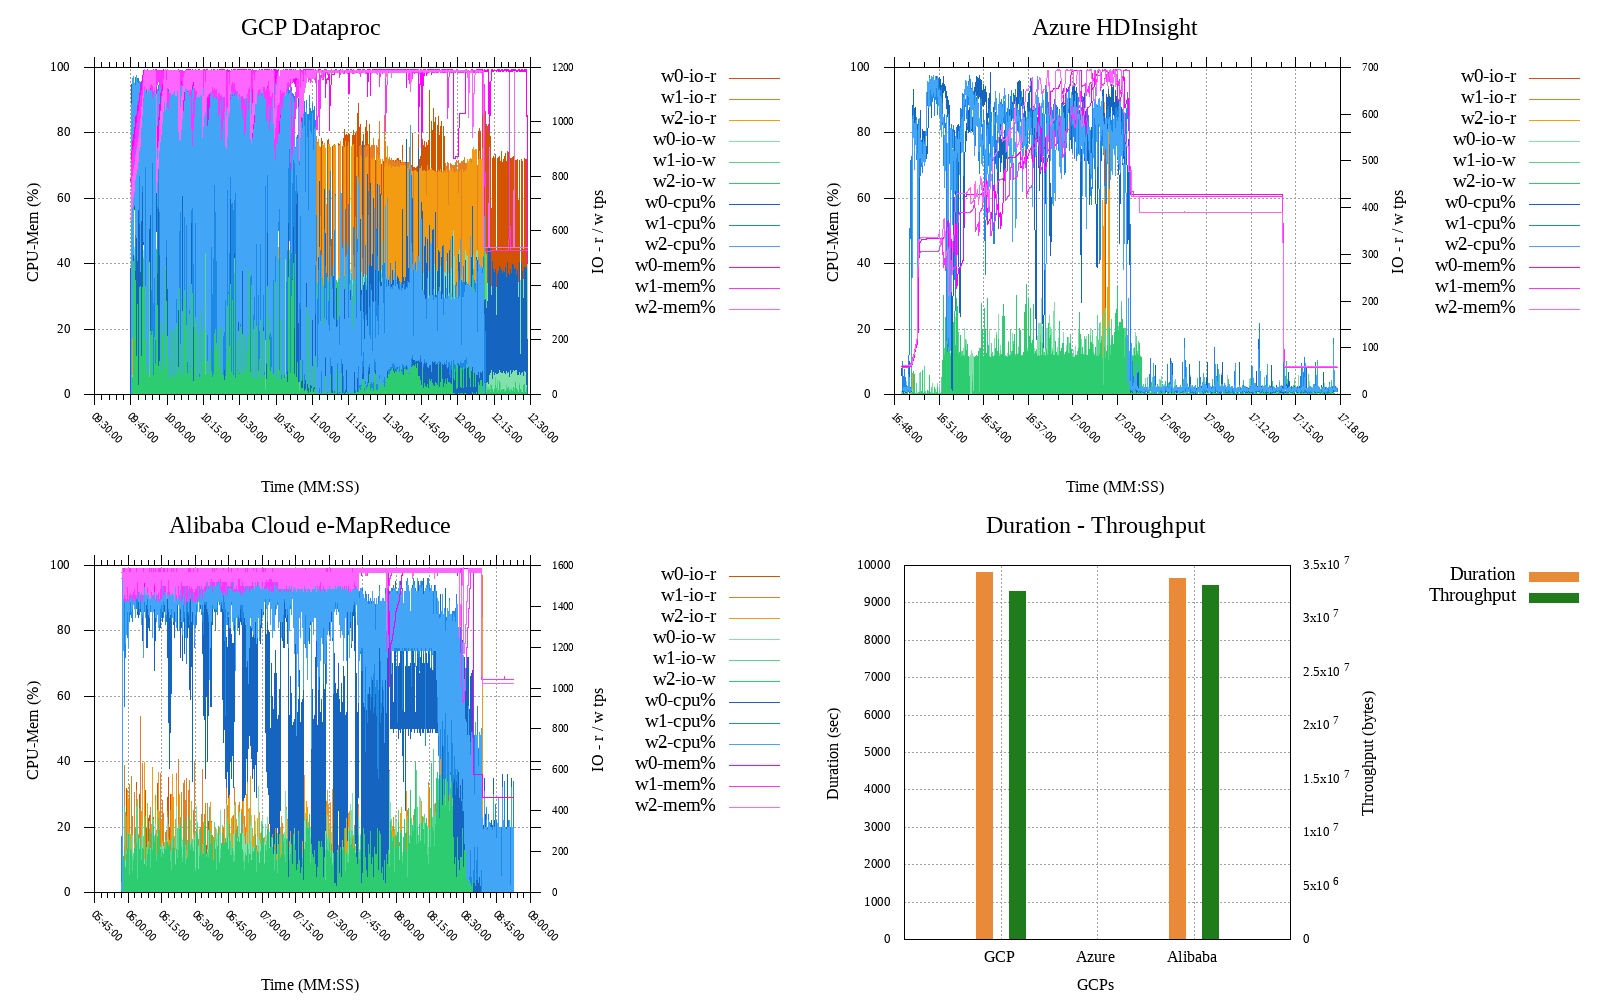
\includegraphics[width=\textwidth]{uc1-tera-g-cmidt}
	\centering
\end{figure}

\subsection{Wordcount}
Figure \ref{fig:uc1-wrdcnt-h-cmidt} shows the results of Wordcount benchmark using Huge scale. GCP performed processor utilization of 75\% to 100\% with a memory consumption between 80\% to 95\% where I/O transfers move along 60 tps peaking at about 150 tps reached second-highest throughput with 978 seconds response time. Azure's processor utilization was moving along 70\% to about 100\%, where memory depicted 30\% to 50\% utilization and lower; I/O transfers peaking at about 60 tps reached the lowest throughput as the most extended duration of 1470 seconds. Alibaba depicted high processor and memory load moving in ranges 70\% to 100\% and 80\% to slightly over 90\%; I/O transfers moving along 200 tps peaking at 300 tps to 350 tps achieved the highest throughput and the shortest execution time of 889 seconds.

\begin{figure}[p]
	\caption{UC1 - Wordcount (Huge; 32 GB)}
	\label{fig:uc1-wrdcnt-h-cmidt}
	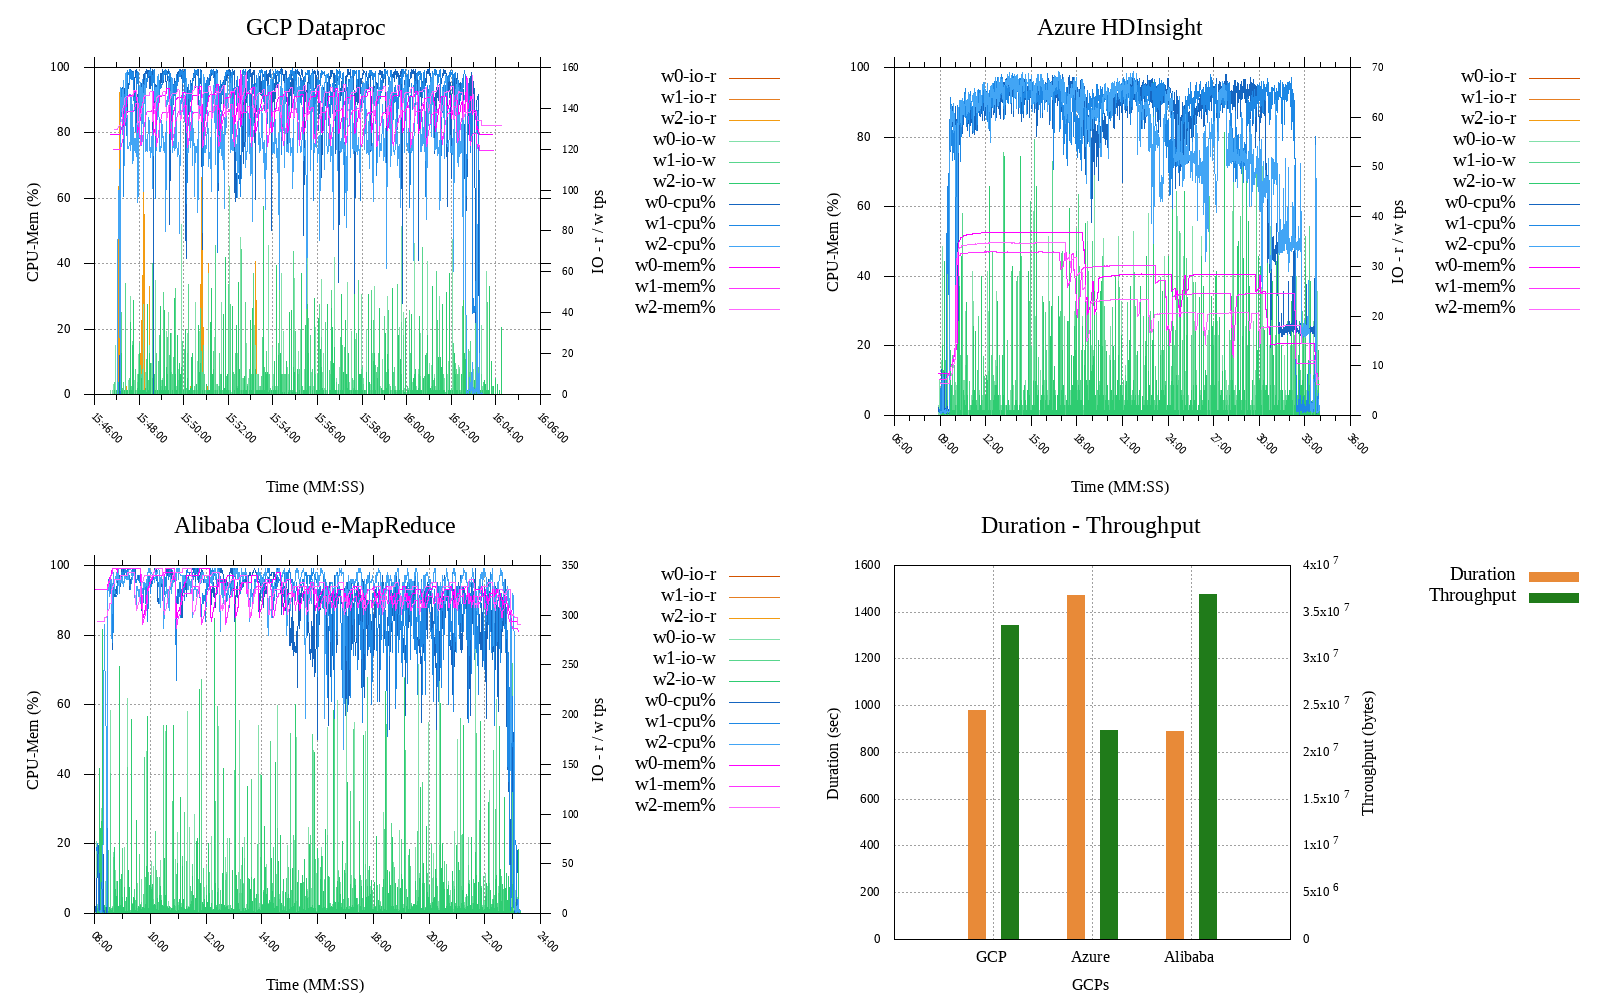
\includegraphics[width=\textwidth]{uc1-wrdcnt-h-cmidt}
	\centering
\end{figure}

In gigantic scale benchmark, GCP utilized processor and memory sources at their maximum during the overall process, for CPU within 60\% up to pushing 100\%, memory utilization varying between 60\% to 100\%, and I/O-read and I/O-write transfers moving along 90 tps and 250 tps, respectively, performed second-highest throughput load resulting in 10131 seconds response time as illustrated in Figure \ref{fig:uc1-wrdcnt-g-cmidt}. Azure showed a dense processor utilization varying between 40\%s and close to 100\%s, memory consumption was somehow oppressed to stay within the range of 20\% up to 50\%, I/O behavior seldomly reacted over 60 tps resulting in the lowest throughput and most extended duration of 13596 seconds. Alibaba demonstrated a high processor utilization within range 85\%-100\%, relatively more stable memory consumption in the range 85\% to 100\%, and I/O transfers mostly about 300 tps, thus performing the highest throughput hence shortest response time of 8671 seconds.

\begin{figure}[p]
	\caption{UC1 - Wordcount (Gigantic; 320 GB)}
	\label{fig:uc1-wrdcnt-g-cmidt}
	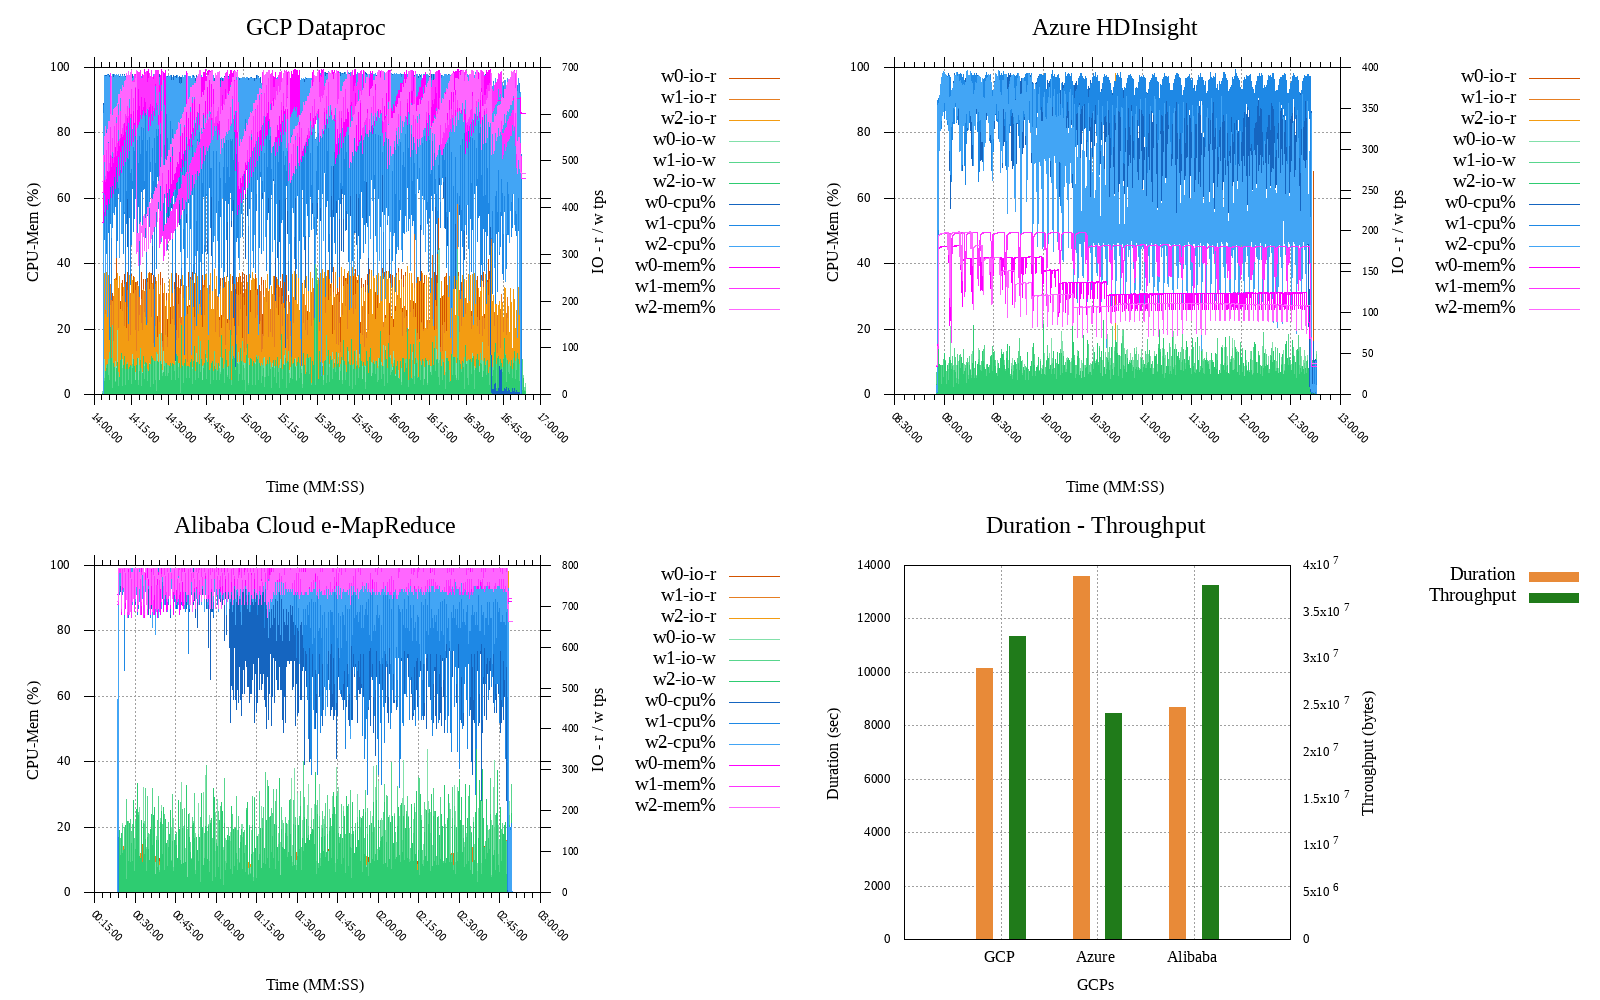
\includegraphics[width=\textwidth]{uc1-wrdcnt-g-cmidt}
	\centering
\end{figure}


\subsection{Dfsioe-read}
GCP's processor utilization is moving roughly between 80\% to 95\%, accompanied by memory utilization within range slightly below and over 70\%, I/O transfers peaking at 400 tps mostly go along 100 tps to 250 tps and performs the second highest throughput resulting in 294 seconds of duration as represented in Figure \ref{fig:uc1-dfsioer-h-cmidt}. Azure's processor utilization is somewhat limited to between 60\% and 90\%, whereas the memory utilization behaves between 10\% to 50\%, generally low I/O transfers with two markable I/O-read and I/O-write condensings reaching peaks at 2000 tps and 1500 tps, respectively, results in the lowest throughput and 662 seconds of response time. With 245 seconds duration, Alibaba displays a similar resource utilization pattern with GCP where it differentiates in memory utilization, moving around 90\%s.

\begin{figure}[p]
	\caption{UC1 - Dfsioe-read (Huge; No of Files: 256, File size: 100 MB)}
	\label{fig:uc1-dfsioer-h-cmidt}
	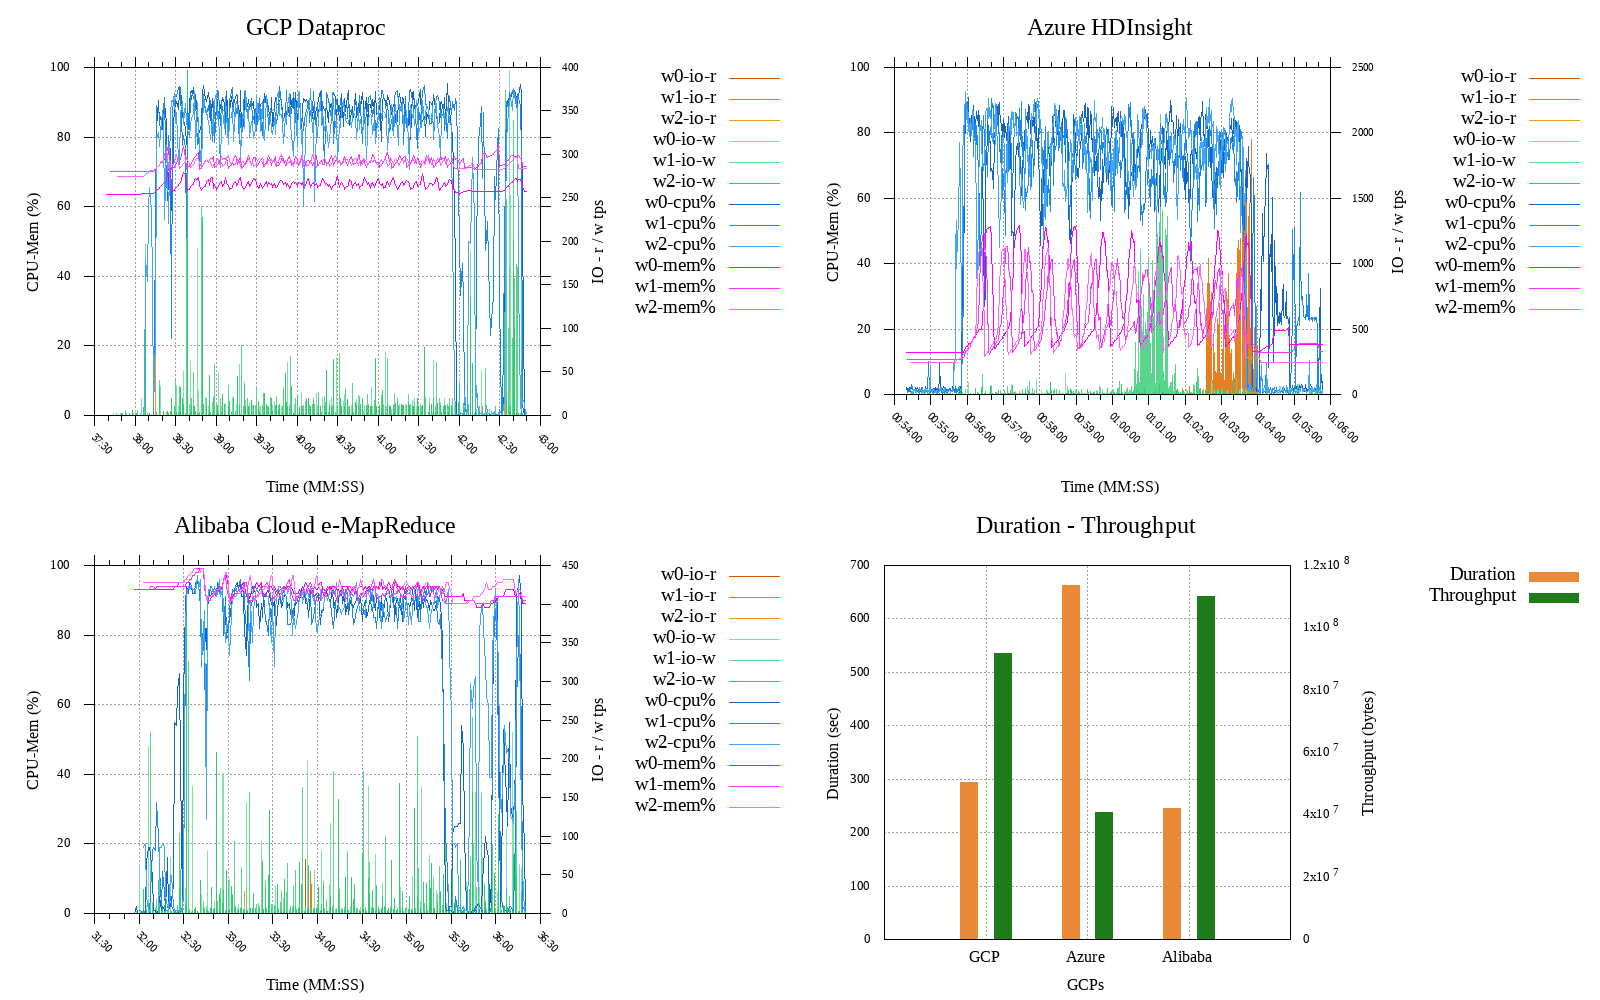
\includegraphics[width=\textwidth]{uc1-dfsioer-h-cmidt}
	\centering
\end{figure}

Figure \ref{fig:uc1-dfsioer-g-cmidt} showed that in gigantic scale, processor utilization in the GCP concentrated within the range of 80\% to 90\%; memory utilization moved around 95\% to 100\%, whereas I/O read transfers executed about 500 tps bringing its performance to the second highest throughput by 915 seconds duration. Azure performed within a range of 55\% up to 90\% in CPU utilization, 20\% to 55\% in memory utilization, and I/O-write activity moving along 70 tps, I/O-read showing a peak at about 470 tps, which results in throughput outputting 1886 seconds response time. Alibaba system utilization was carried out around 80\%-90\% range for processing performance, 90\%-100\% for memory load, and behavior up to 1700 tps I/O-write placing its performance to the highest throughput with 660 seconds duration.

\begin{figure}[p]
	\caption{UC1 - Dfsioe-read (Gigantic; No of Files: 512, File size: 400 MB)}
	\label{fig:uc1-dfsioer-g-cmidt}
	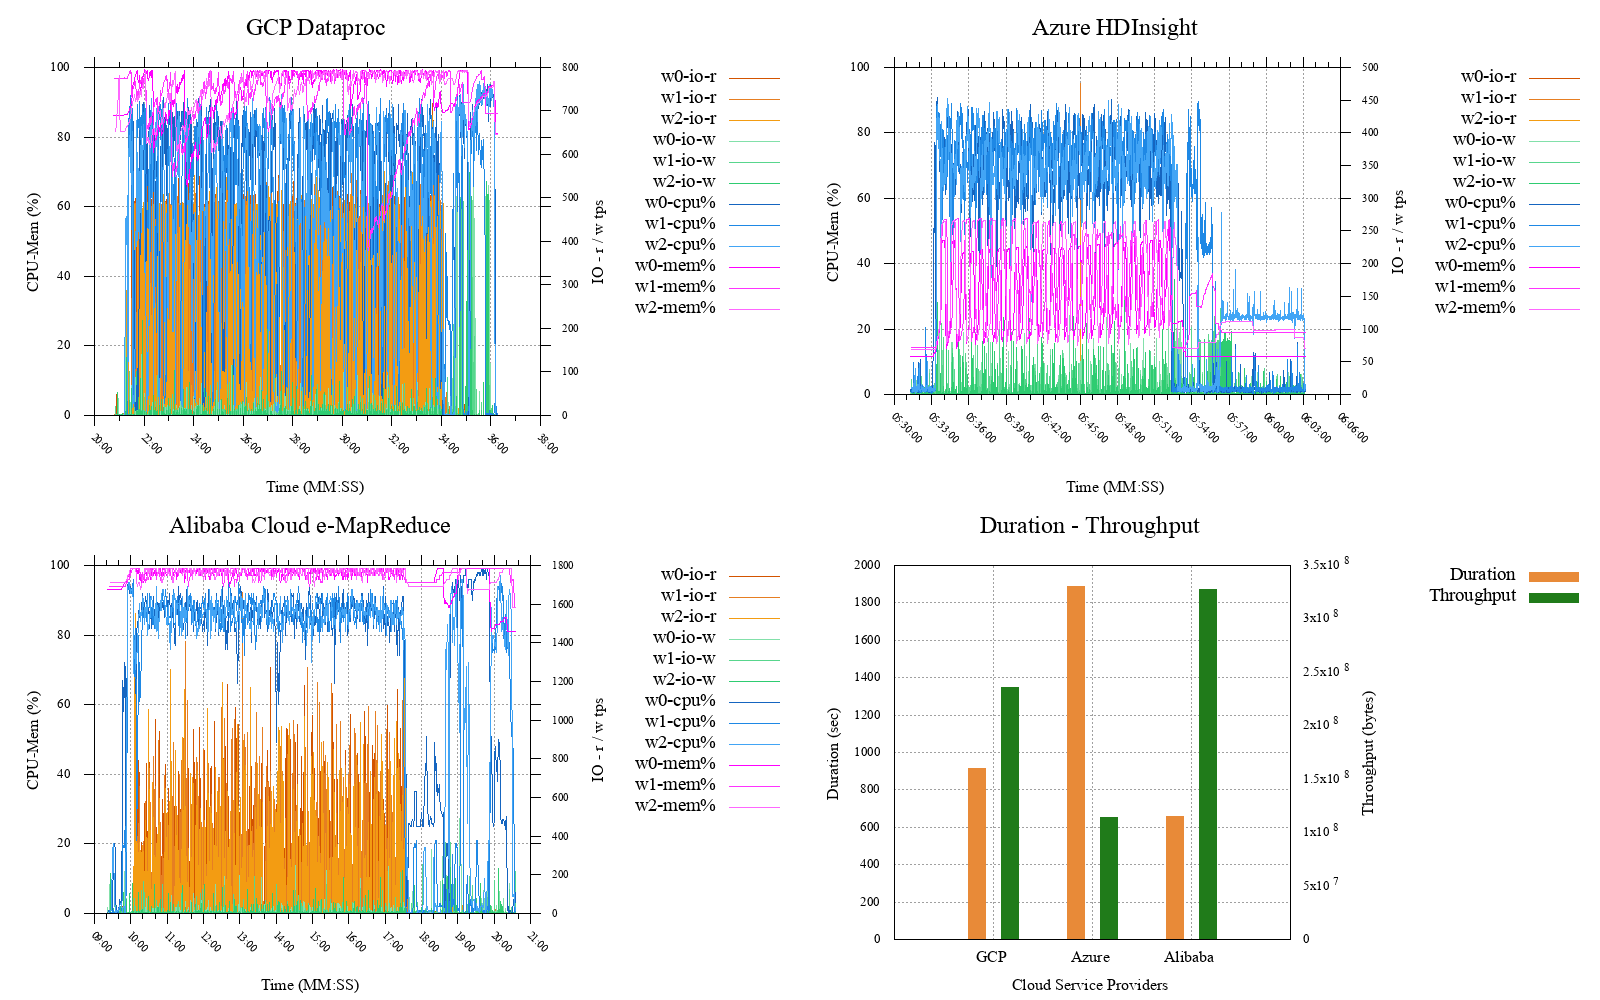
\includegraphics[width=\textwidth]{uc1-dfsioer-g-cmidt}
	\centering
\end{figure}

\subsection{Dfsioe-write}
In Dfsioe-write benchmark, GCP's processor utilization was realized between 70\% and 90\%, memory load increments from 20\% up to 70\%, whereas I/O-write transfers achieved 500 tps resulting in the second shortest response time 379 seconds as depicted in Figure \ref{fig:uc1-dfsioew-h-cmidt}. Azure's CPU utilization was around 60\% to 90\%, memory load fluctuated between 20\% and 40\%, whereas I/O-write transfers varied about 20 tps to 80 tps, peaking at about 120 tps by a duration output of 658 seconds. Alibaba performed the heaviest throughput with processor utilization 80\% and 95\%, memory load increments from about 40\% up to 90\%-100\%, and I/O-write transfers at about 100 tps to 600 tps, peaking at about 800 tps, and reached the shortest response time with 281 seconds.

\begin{figure}[p]
	\caption{UC1 - Dfsioe-write (Huge; No of Files: 256, File size: 100 MB)}
	\label{fig:uc1-dfsioew-h-cmidt}
	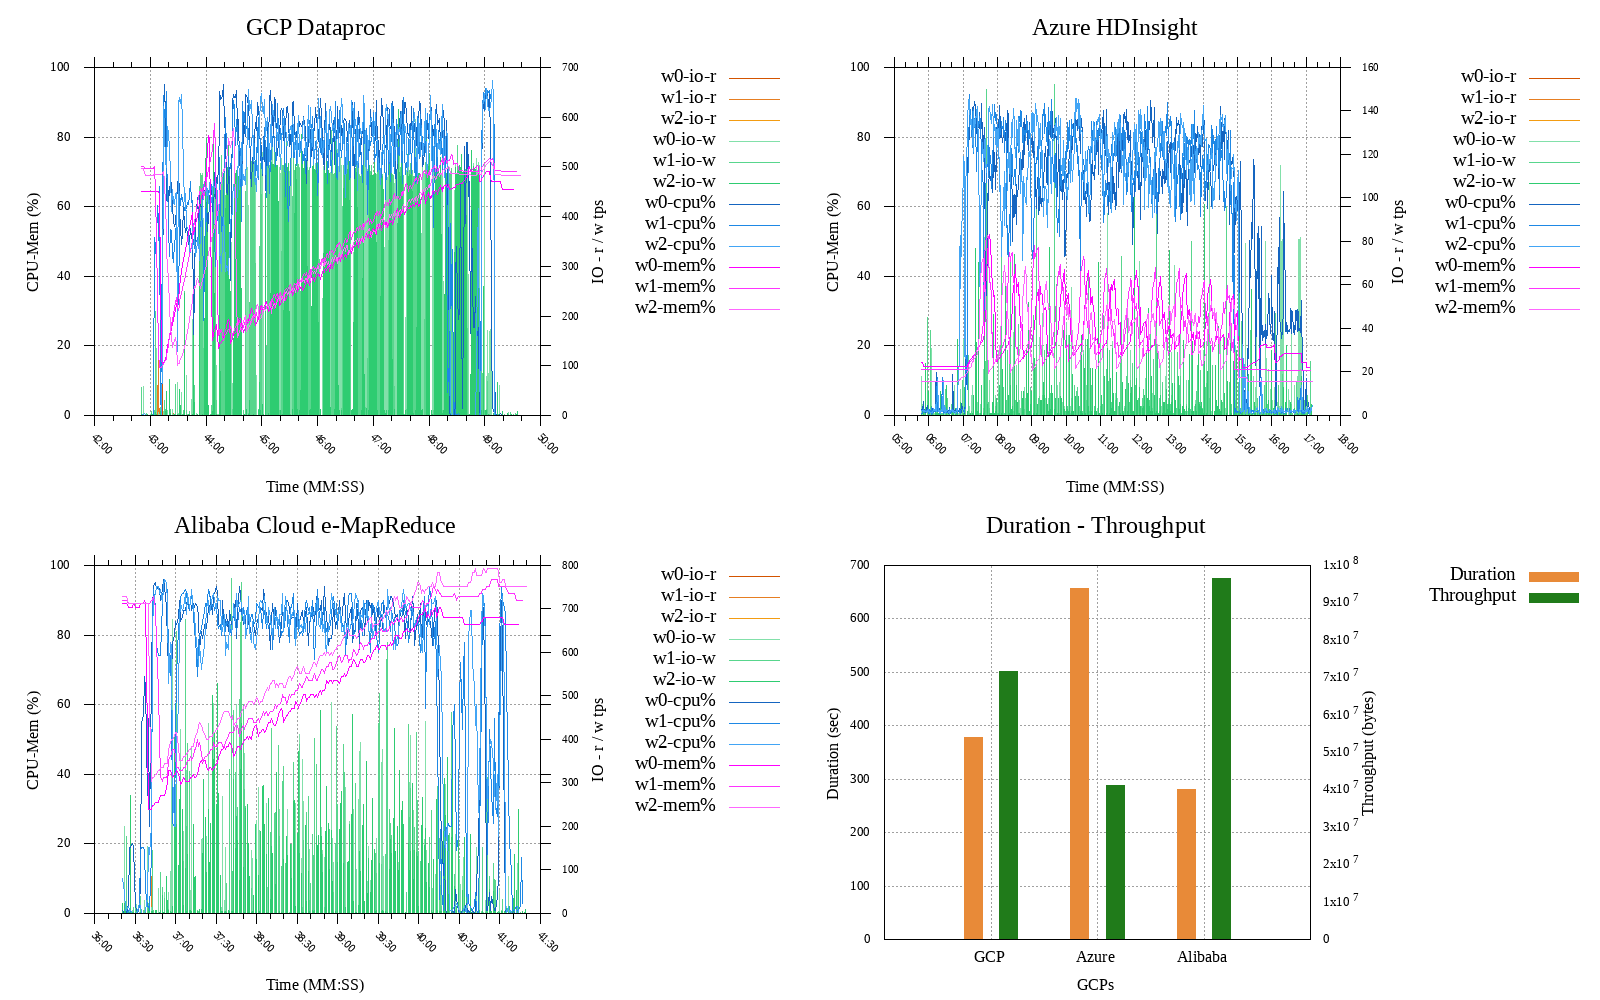
\includegraphics[width=\textwidth]{uc1-dfsioew-h-cmidt}
	\centering
\end{figure}

GCP processor utilization in gigantic scale shifted along a broad range hitting up to 90\% load, memory load quickly rises to 95\%-100\% range and keeps its position in overall execution, I/O-writes move along 500 tps to 600 tps placing GCP to the second-best performance with 1347 seconds response time. Azure shows a CPU utilization in a range of 60\% up to 90\% until it drops to about 25\% in the 2/3th of the overall process, memory load moves along lower 20\% to upper 50\% until its sudden drop to upper 15\% simultaneously with CPU utilization where I/O-write transfers peak at about 120 tps resulting in 1914 seconds response time as appeared in Figure \ref{fig:uc1-dfsioew-g-cmidt}. Alibaba performing the shortest response time with 1060 seconds displays a similar memory and processor utilization behavior with GCP where it differs in I/O-write transfers peaking at about 900 tps.

\begin{figure}[p]
	\caption{UC1 - Dfsioe-write (Gigantic; No of Files: 512, File size: 400 MB)}
	\label{fig:uc1-dfsioew-g-cmidt}
	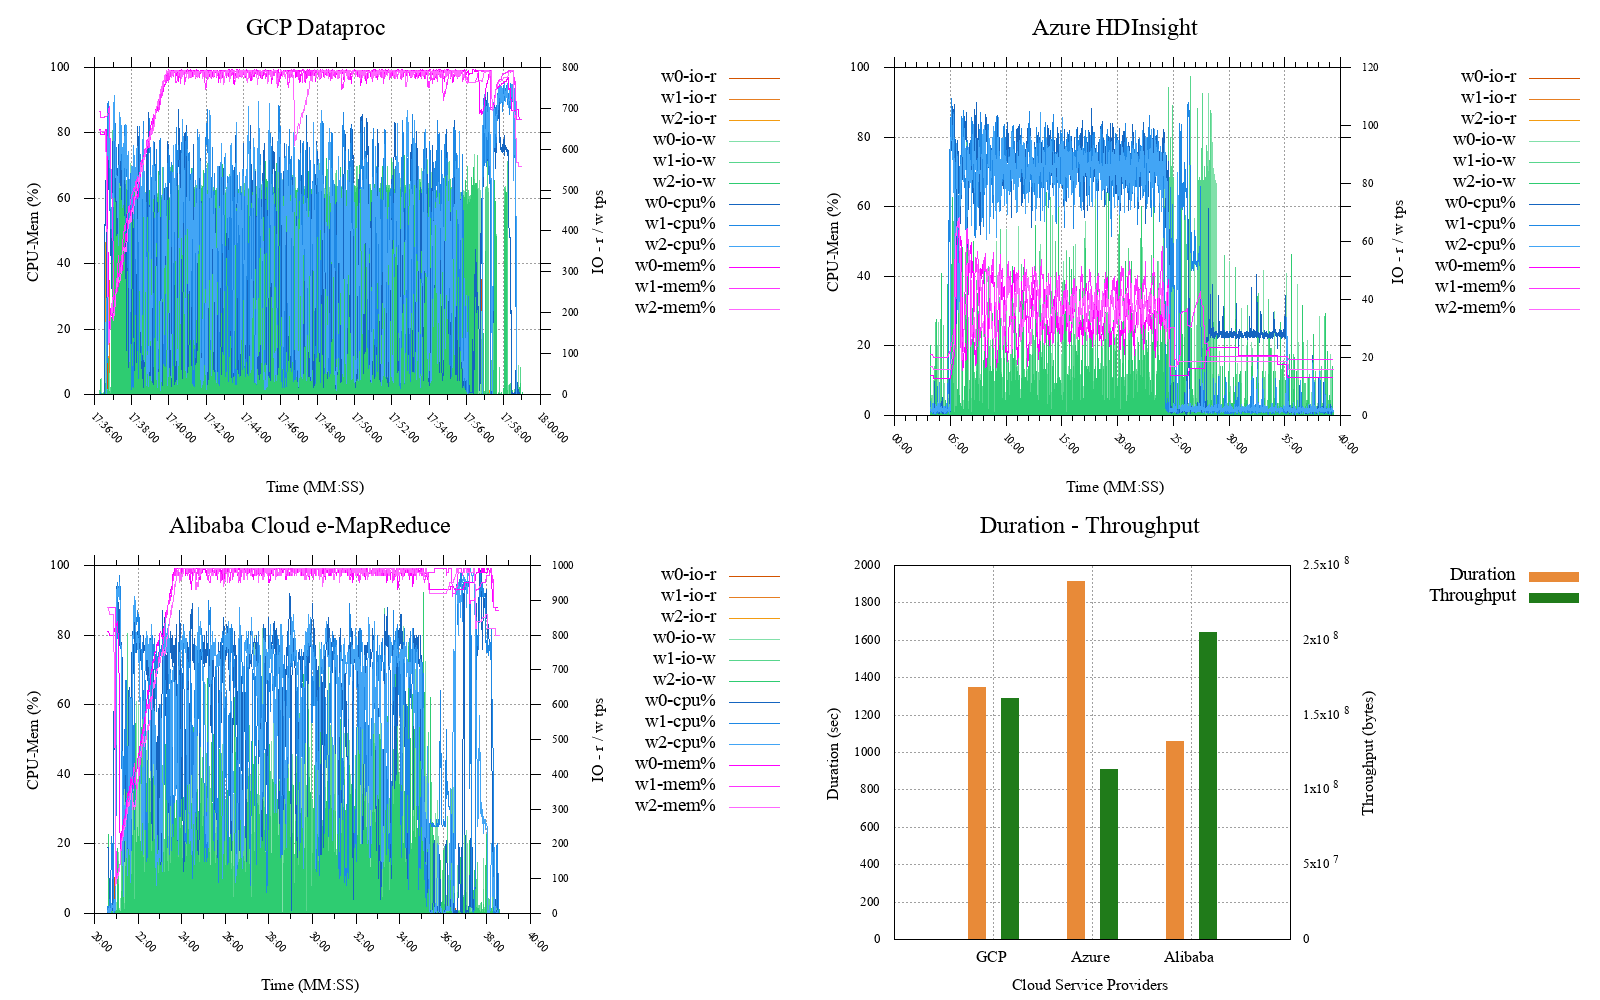
\includegraphics[width=\textwidth]{uc1-dfsioew-g-cmidt}
	\centering
\end{figure}

\subsection{Scan}
The results of Scan benchmark illustrated in Figure \ref{fig:uc1-scan-h-cmidt} that GCP processor utilization condensed between about 80\% and 90\% during benchmark execution; memory load changed between 20\% and 40\%, accompanied by an I/O-write transfer reaching over 500 tps, which brought GCP to the top performance within this benchmark with 73 seconds. On Azure's side, processor utilization deviated in 80\%-90\% range, whereas memory load incremented from the 15\%s to the 30\%s, relatively low I/O-write transfers peaked at nearly 85 tps, which resulted in lowest throughput and 157 seconds duration. Alibaba followed a similar pattern like GCP in resource utilization with about 90\% CPU load, 15\% to below 40\% memory utilization but a less dense I/O-write transfer topped at about 550 tps and so achieving a similar throughput to GCP resulting in 74 seconds response time.

\begin{figure}[p]
	\caption{UC1 - Scan (Huge; USERVISITS: 10,000,000 PAGES: 1,200,000)}
	\label{fig:uc1-scan-h-cmidt}
	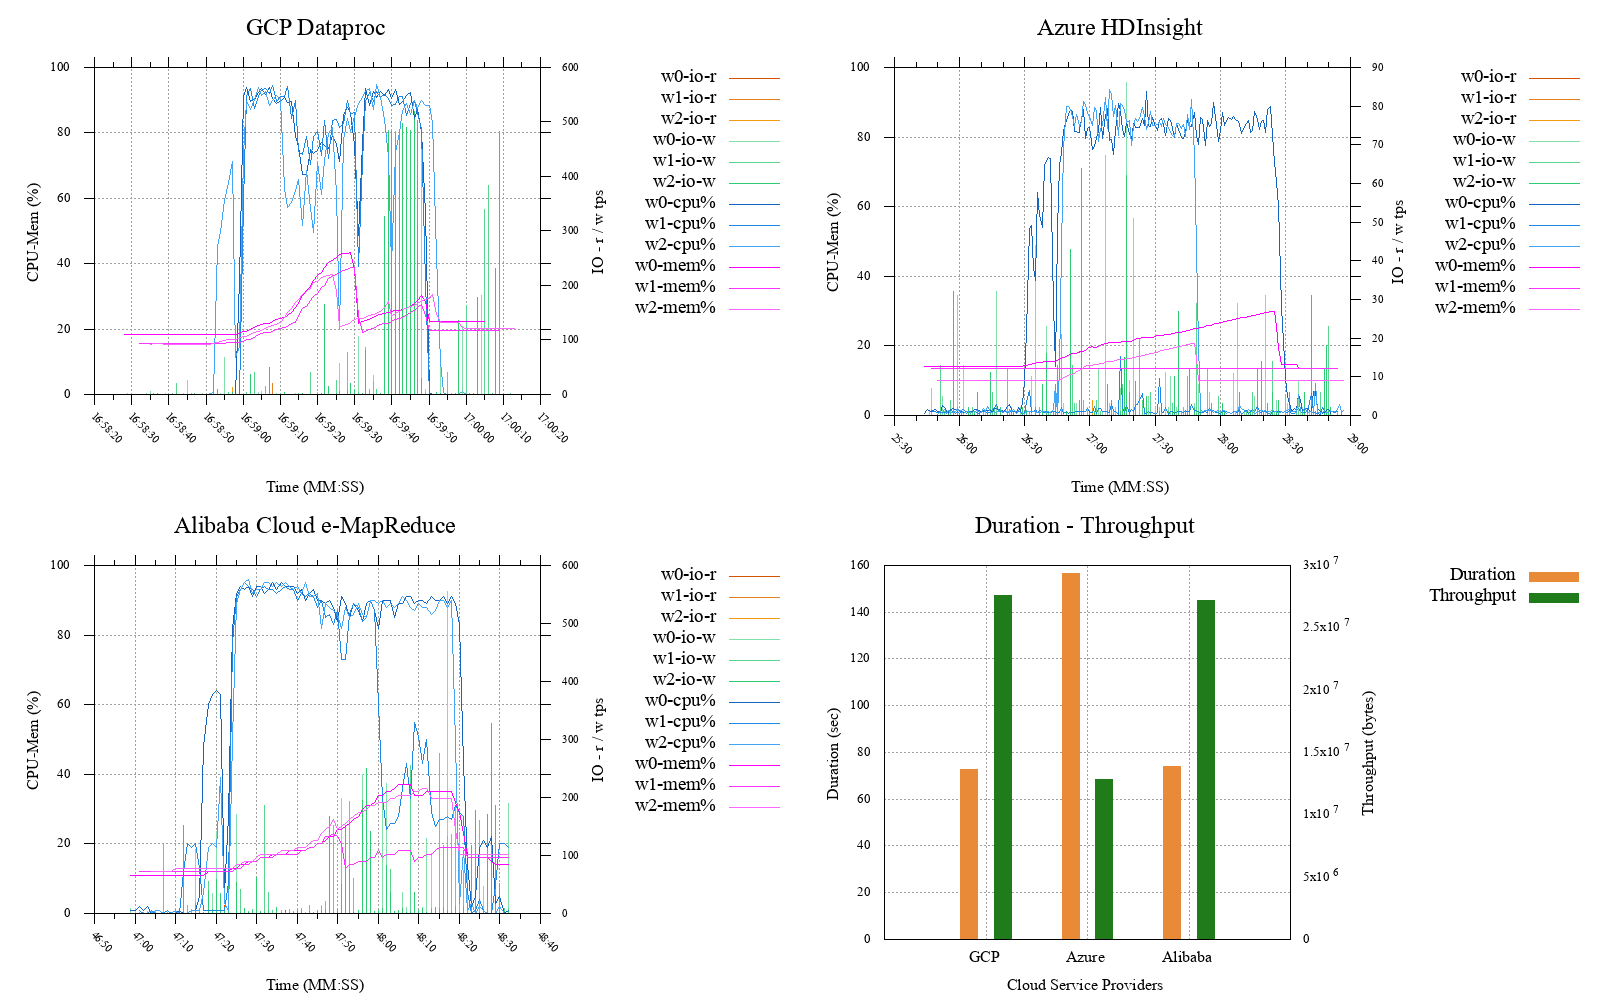
\includegraphics[width=\textwidth]{uc1-scan-h-cmidt}
	\centering
\end{figure}

GCP's CPU utilization in gigantic scale benchmark varied between 50\%s and 90\%s with convergence at about 80\%s, memory load showed similar range with utilization reaching up 100\%s and I/O-write transfers shifted between 500 tps and 600 tps results in second-highest throughput by a 457 seconds response time as indicated in Figure \ref{fig:uc1-scan-g-cmidt}. Azure's CPU utilization condensed between 80\% and 90\% and memory load incremented two times from 20\%s to 40\%s, I/O-write transfers performed nearby 50 tps to 60 tps, peaking at about 200 tps results in 514 seconds duration. A relatively higher Alibaba's processor utilization was observed in range of 80\% and 95\%, increased memory load ranging from 40\%s-50\%s to 80\%s-100\%s during runtime and I/O-write transfers exceeding over 500 tps results in the highest throughput, thus, the shortest duration of 407 seconds.

\begin{figure}[p]
	\caption{UC1 - Scan (Gigantic; USERVISITS: 100,000,000 PAGES: 12,000,000)}
	\label{fig:uc1-scan-g-cmidt}
	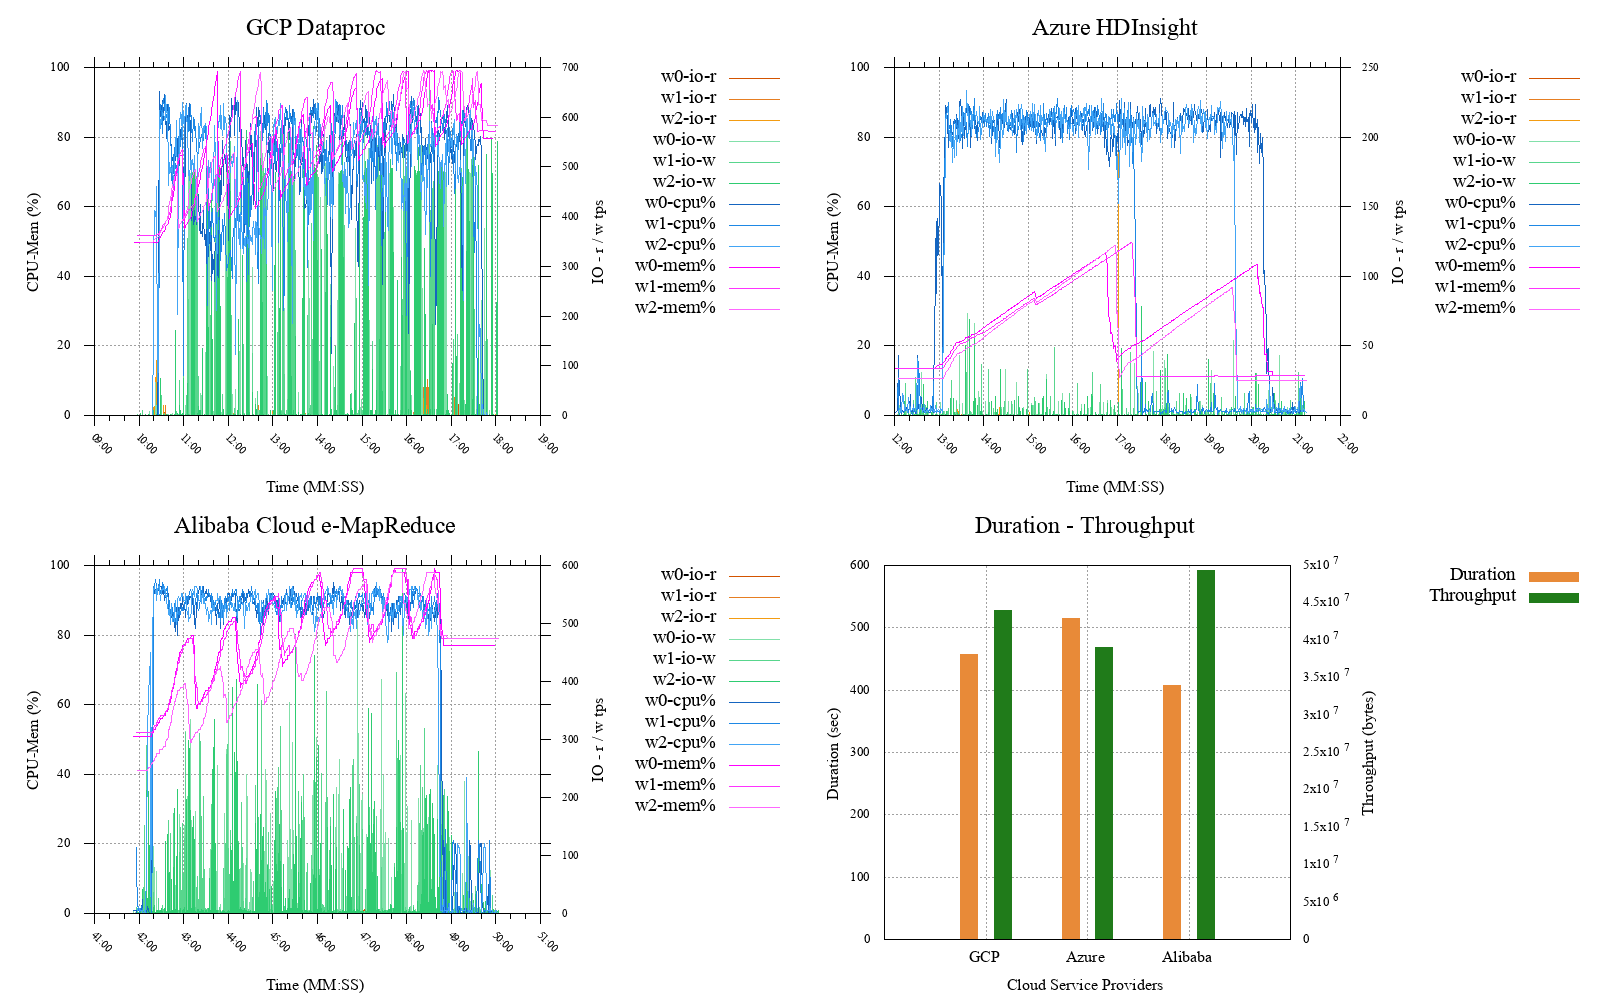
\includegraphics[width=\textwidth]{uc1-scan-g-cmidt}
	\centering
\end{figure}

\subsection{Join}
In Join benchmark with huge scale, GCP processor load changed mainly between 80\%s and over 90\%s; memory utilization varied along 20\%s and 30\%s, I/O-writes executed at about 150 tps, brought outputs to 181 seconds response time as appeared in Figure \ref{fig:uc1-join-h-cmidt}. Azure's resource utilization performed at a range between 80\% and 90\% for CPU, varying memory loads moved along 20\%s and below 60\%s, I/O-write transfers executed below 60 tps with a peak of 100 tps resulting in a lower throughput and response time of 356 seconds. Resource utilization at Alibaba appeared similarly to GCP in processor and memory load, whereas I/O-write peaked at about 260 tps, reached the highest throughput and a duration of 175 seconds.


\begin{figure}[p]
	\caption{UC1 - Join (Huge; USERVISITS: 10,000,000 PAGES: 1,200,000)}
	\label{fig:uc1-join-h-cmidt}
	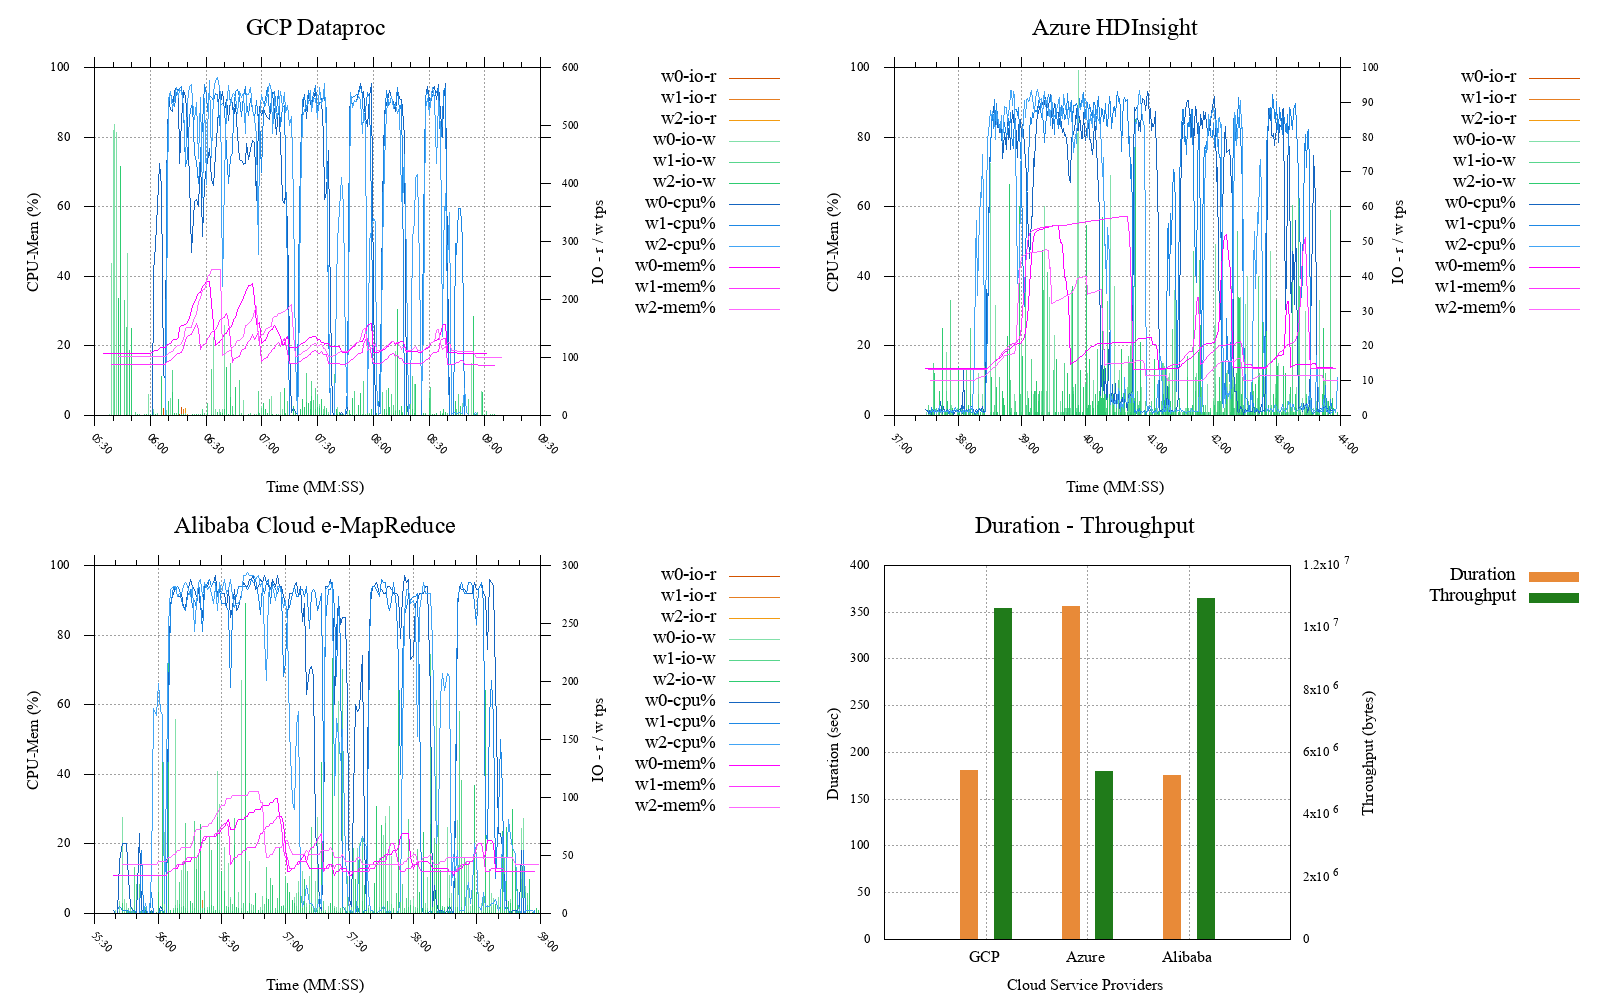
\includegraphics[width=\textwidth]{uc1-join-h-cmidt}
	\centering
\end{figure}

It is observed in Figure \ref{fig:uc1-join-g-cmidt} that CPU load in GCP performed around 70\% to 90\% overall, whereas RAM utilization among worker nodes was within 50\% to 90\% range, I/O-write transfers observed in behavior about 100 tps resulting in a throughput outputting 595 seconds of response time for Join task in Gigantic setting. Azure's performance dynamics indicated a load of 80\% to 90\% with decreasing utilization on some worker nodes in a later stage, memory utilization moving along the range of 20\% up to 60\%, and I/O-write transfer observations topped at 120 tps, provided the lowest throughput, consequently, the longest response time of 761 seconds.  The processor utilization of Alibaba was approximately 90\% to 100\%, memory load behavior changed along 50\% to below 70\%, and I/O-write observation peaked at 350 tps, performed a slightly higher throughput than GCP, for a slightly shorter duration of 594 seconds.

\begin{figure}[p]
	\caption{UC1 - Join (Gigantic; USERVISITS: 100,000,000 PAGES: 12,000,000)}
	\label{fig:uc1-join-g-cmidt}
	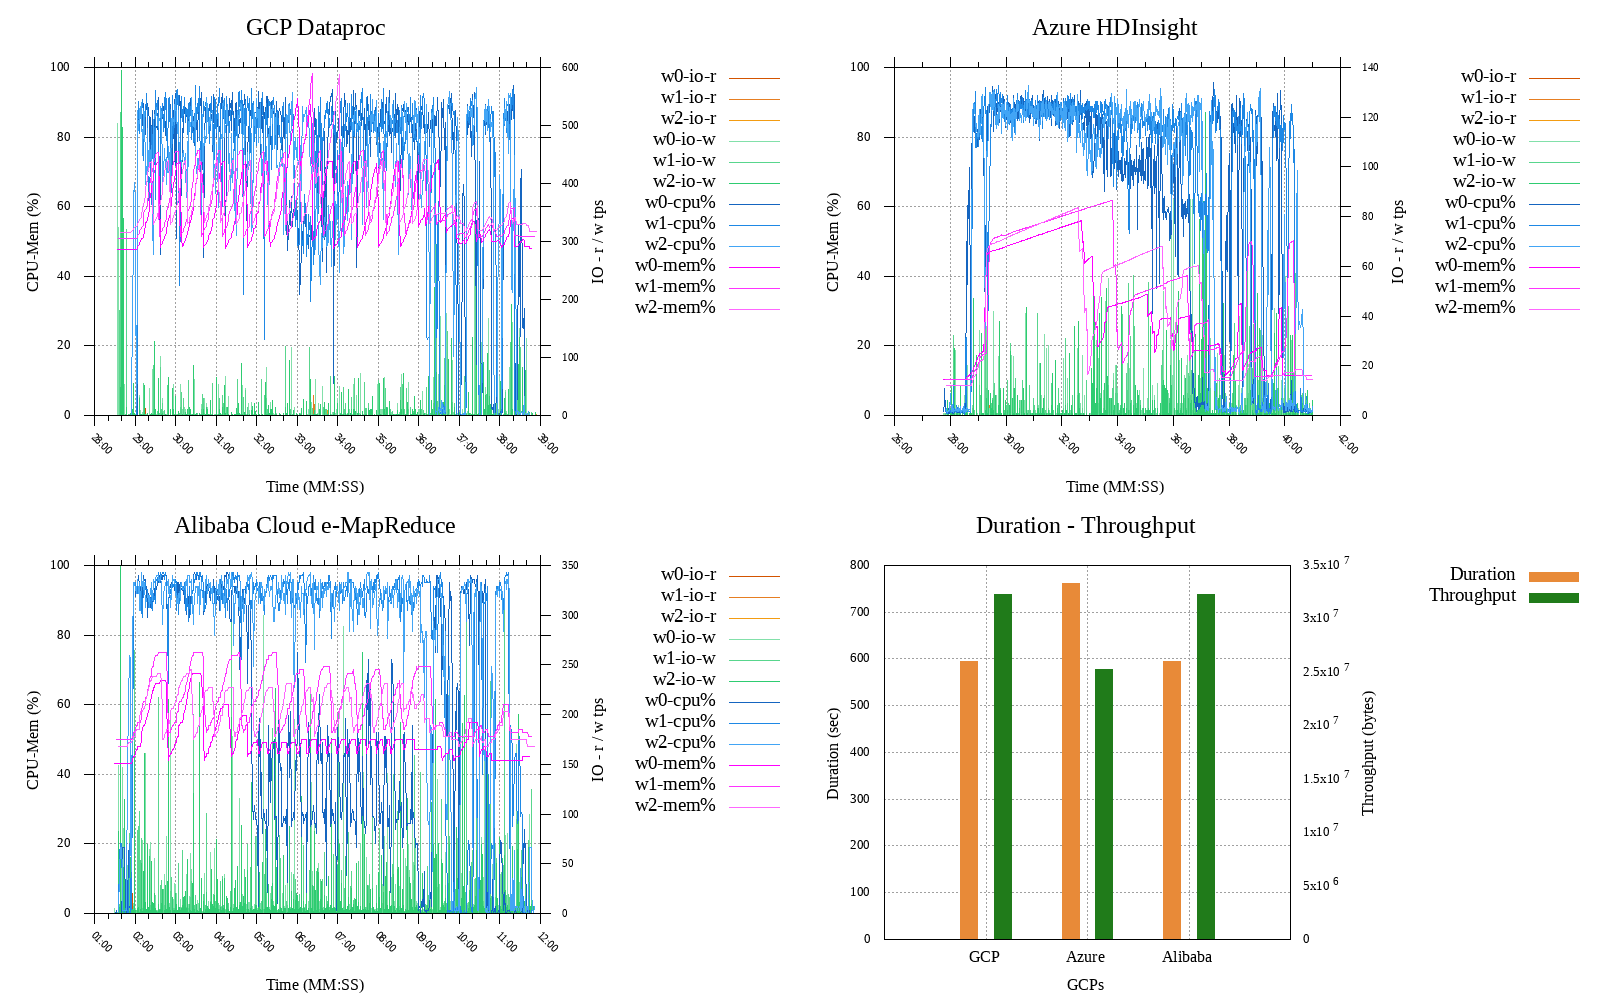
\includegraphics[width=\textwidth]{uc1-join-g-cmidt}
	\centering
\end{figure}


\subsection{Aggregation}
In the Aggregation benchmark results, it is noticed that GCP processor utilization was carried out between 80\% and 95\%, memory load changed between 15\% to 40\%, and I/O-write transfer observed at about 150 tps result in 97 seconds. Azure's CPU utilization varied between 80\% and 90\%, whereas memory load performed around from 10\% to varying utilization among worker nodes up to 30\% and below 60\%, and I/O-write transfers reached at about 180 tps, performed a relatively small throughput resulting in 215 seconds completion time. Alibaba resource utilization was between 80\% and 90\% for CPU, 10\% to 40\% in memory, and I/O-write transfer average of 26 tps showed comparable performance to GCP resulting in the same completion time of 97 seconds as shown in Figure \ref{fig:uc1-aggreg-h-cmidt}.
 
\begin{figure}[p]
	\caption{UC1 - Aggregation (Huge; USERVISITS: 10,000,000 PAGES: 1,200,000)}
	\label{fig:uc1-aggreg-h-cmidt}
	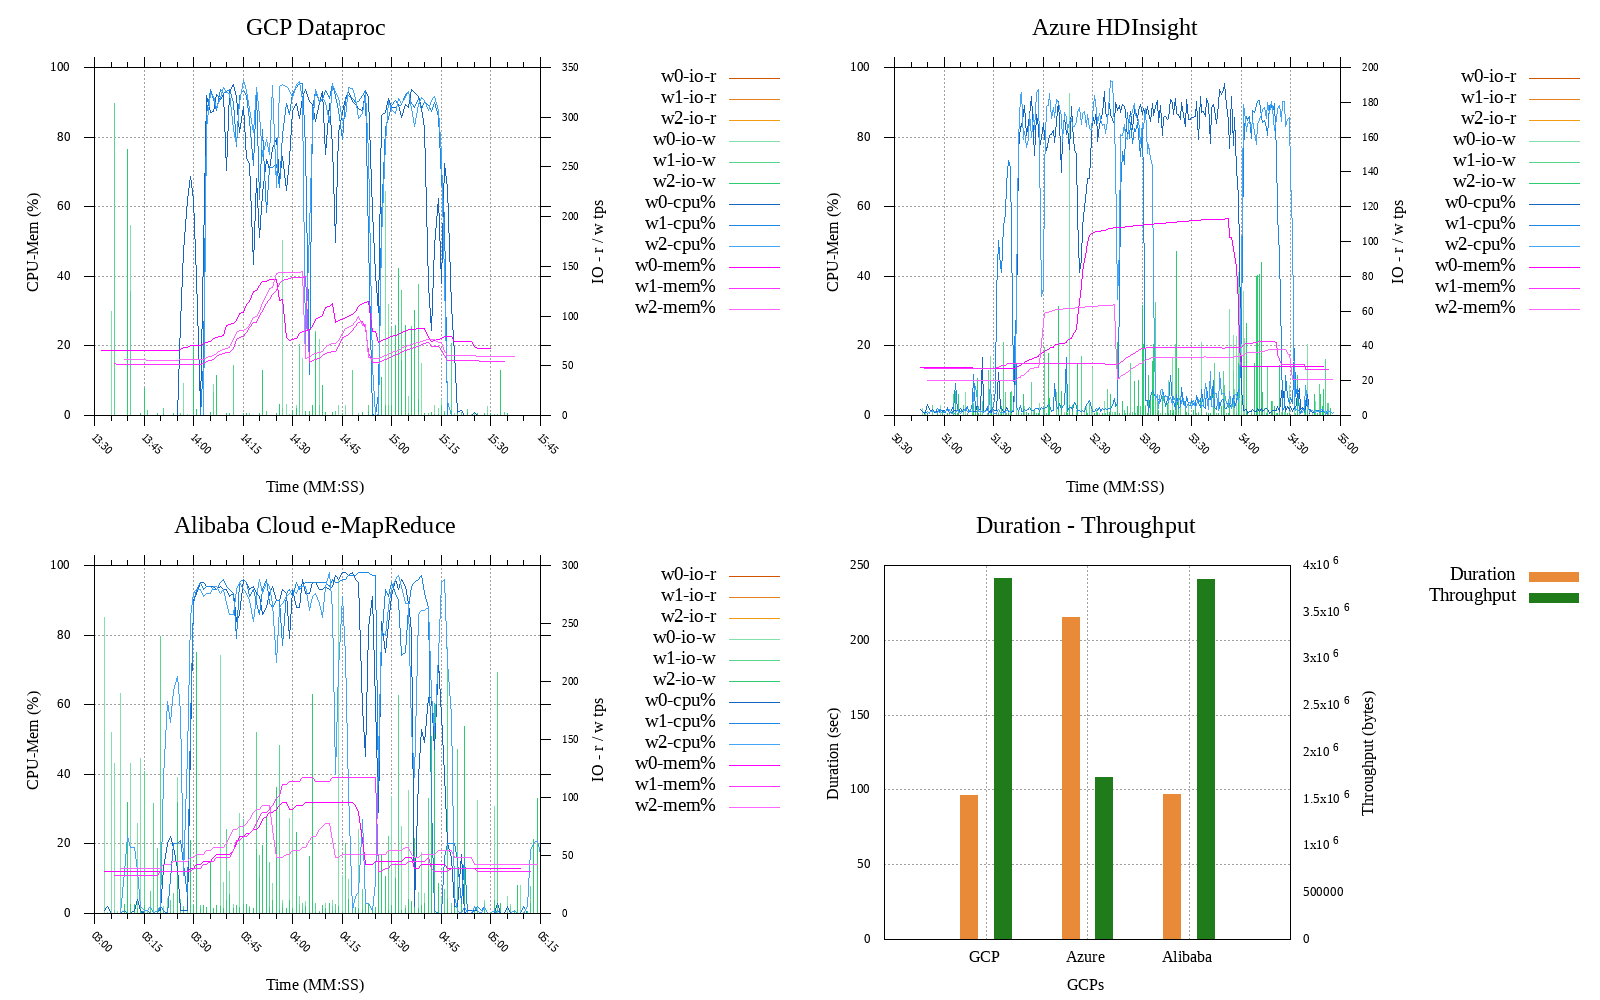
\includegraphics[width=\textwidth]{uc1-aggreg-h-cmidt}
	\centering
\end{figure}

Using gigantic dataset, the processor utilization of GCP altered between 80\% and 90\% in overall execution, memory load between 50\% and 70\% peaking to below 100\%, I/O-write transfers reached a dense behavior at the end reaching 500 tps results in highest throughput and 523 seconds response time. Azure displayed a CPU utilization of below 80\% to above 90\%, mild RAM utilization moving along 30\%s to 60\%s, I/O-write transfers were about 100 tps resulting in relatively low throughput and 594 seconds of duration to complete. Alibaba's processor load moved along 80\% to below 100\%, I/O-write transfer behavior scaling from about 50 tps to 400 tps results in 565 seconds response time as shown in Figure \ref{fig:uc1-aggreg-g-cmidt}.

\begin{figure}[p]
	\caption{UC1 - Aggregation (Gigantic; USERVISITS: 100,000,000 PAGES: 12,000,000)}
	\label{fig:uc1-aggreg-g-cmidt}
	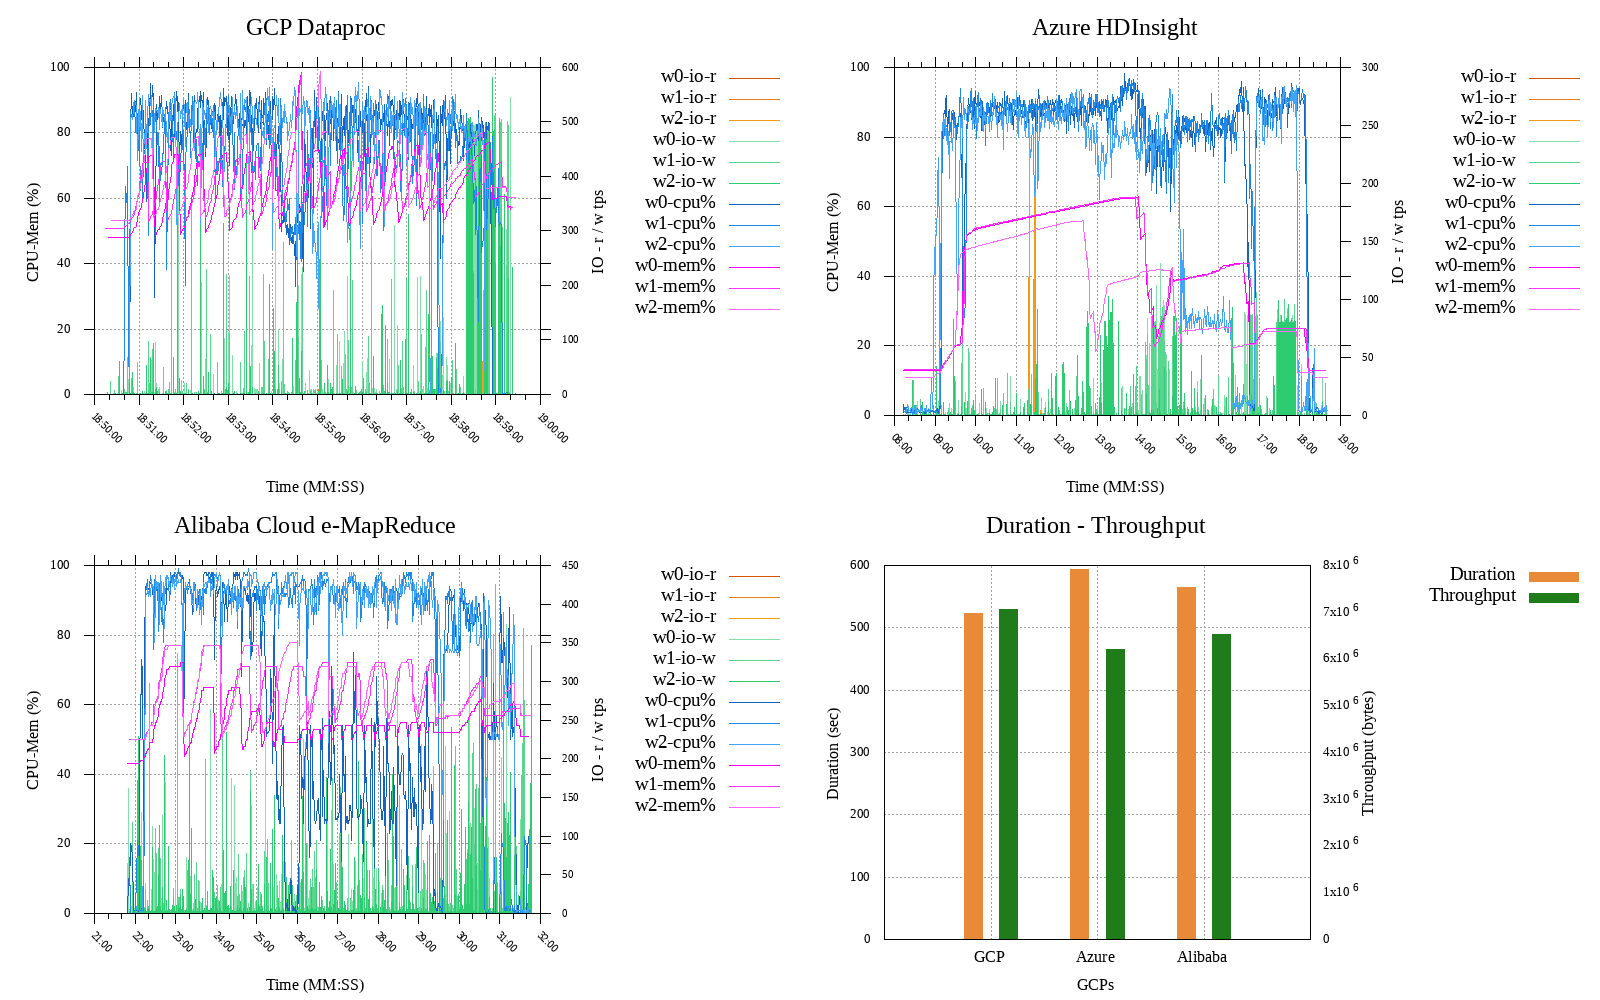
\includegraphics[width=\textwidth]{uc1-aggreg-g-cmidt}
	\centering
\end{figure}

\subsection{Bayes}
In the Bayes benchmark results with Huge dataset, Google CP in processor behavior performed at around 70\%s to below 100\%, memory load at about 30\% with a short peak to below 100\% at the first half, and I/O-write transfers accomplished approximately 500 tps, resulting in highest throughput thus fastest response time of 2604 seconds as clearly demonstrated in Figure \ref{fig:uc1-bayes-h-cmidt}. Azure displayed a split behavior in CPU utilization among worker nodes, where one load moved at about 80\% to lower 100\% and one node depicted a movement on the minimum at about 20\%; memory load on worker nodes also varied from each other by about 20\% load difference at the beginning however meeting the similar range starting at the second half, I/O observations depicted a low range with the exception at the high I/O-write transfer at about 3200 tps at the initial state of the execution resulted in a relatively low throughput, accordingly, the most prolonged duration of 6120 seconds. Alibaba CPU utilization showed varieties among worker nodes in load ranges; RAM utilization condensed at higher levels of 80\%, I/O transfers moved along 100 tps to observable 450 tps resulting in 3017 seconds response time.

\begin{figure}[p]
	\caption{UC1 - Bayes (Huge; PAGES: 500,000 CLASSES: 100 NGRAMS: 2)}
	\label{fig:uc1-bayes-h-cmidt}
	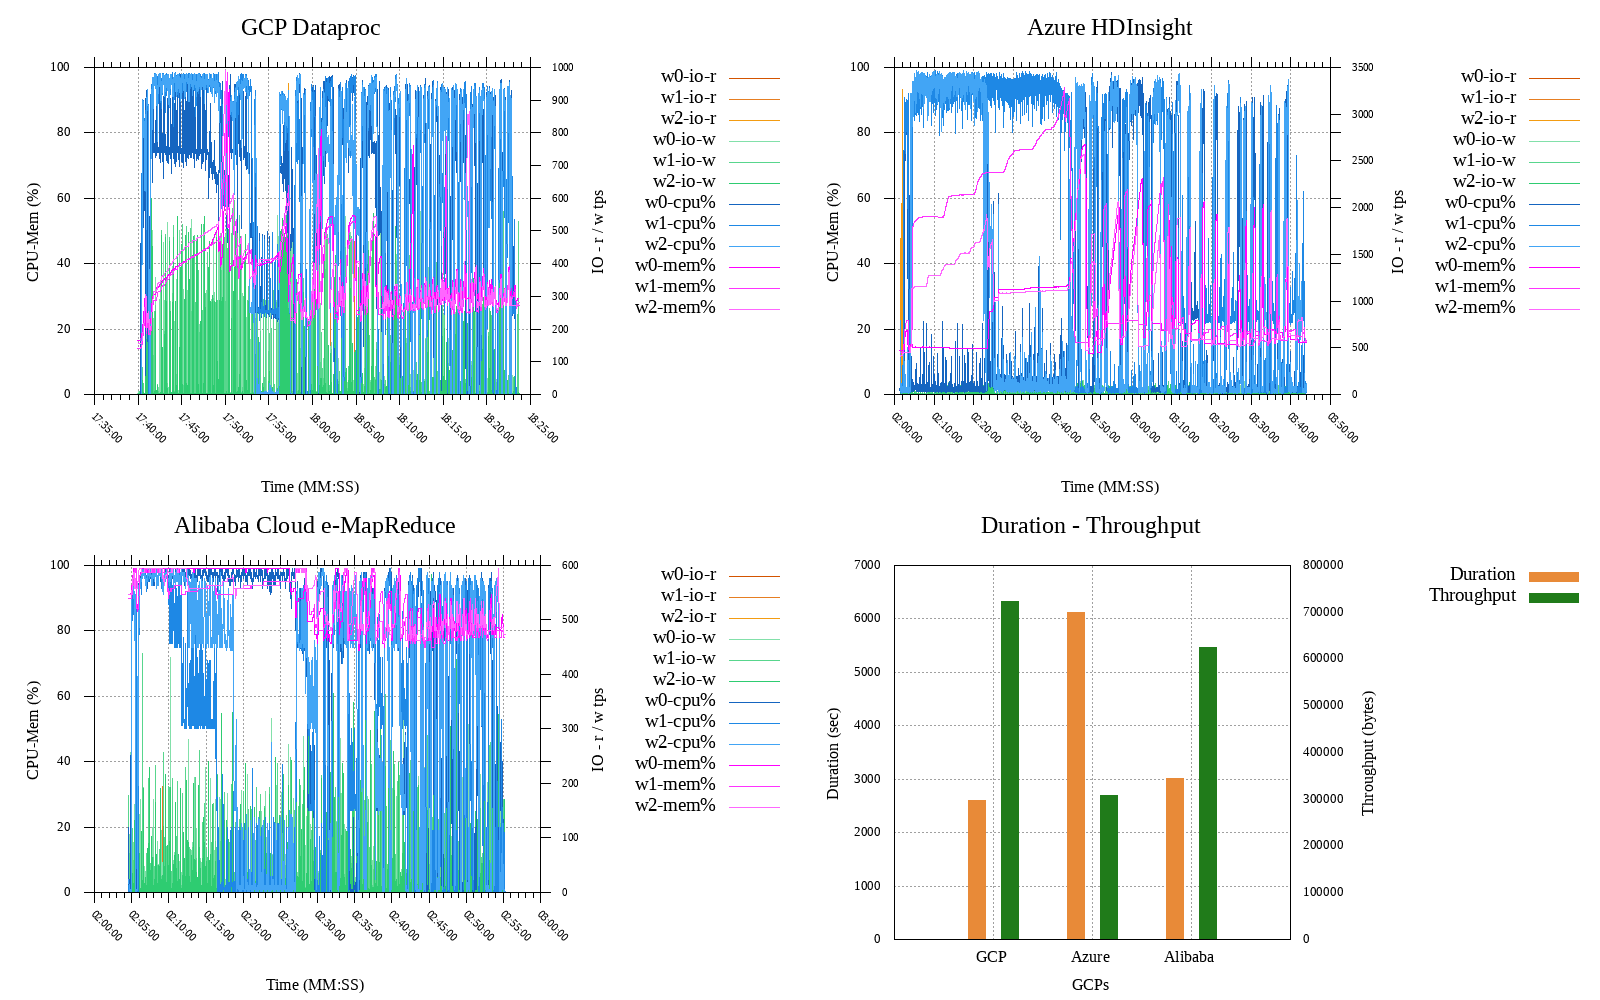
\includegraphics[width=\textwidth]{uc1-bayes-h-cmidt}
	\centering
\end{figure}

From the results of Bayes task using gigantic dataset, it is obtained that GCP's processor utilization was approximating in range of 70\% to 100\%, accompanied by memory load increments from 40\%s to 70\%s becoming stable at 50\%s, and I/O-write transfers were nearly 500 tps, which resulted in the highest throughput and 5350 seconds of response time. Azure's resource utilization showed the distinction in CPU and memory among worker nodes while two nodes depicted higher utilization at about 70\% to below 100\% for processing and 40\%-50\% for memory, one node staying at lower levels for respective resources, the observed I/O-write transfer moved along 100 tps where I/O-read transfer peaks at about 650 tps resulting in the lowest performance of 12589 seconds duration. Alibaba provided different utilization ranges among worker nodes for processing, the memory consumption followed a more balanced load among worker nodes with I/O-write transfer moved along 200 tps, which is a relatively lower throughput, hence, the relatively long duration of 6363 seconds, with respect to GCP. Figure \ref{fig:uc1-bayes-g-cmidt} displays the comparison results for the cloud providers.

\begin{figure}[p]
	\caption{UC1 - Bayes (Gigantic; PAGES: 1,000,000 CLASSES: 100 NGRAMS: 2)}
	\label{fig:uc1-bayes-g-cmidt}
	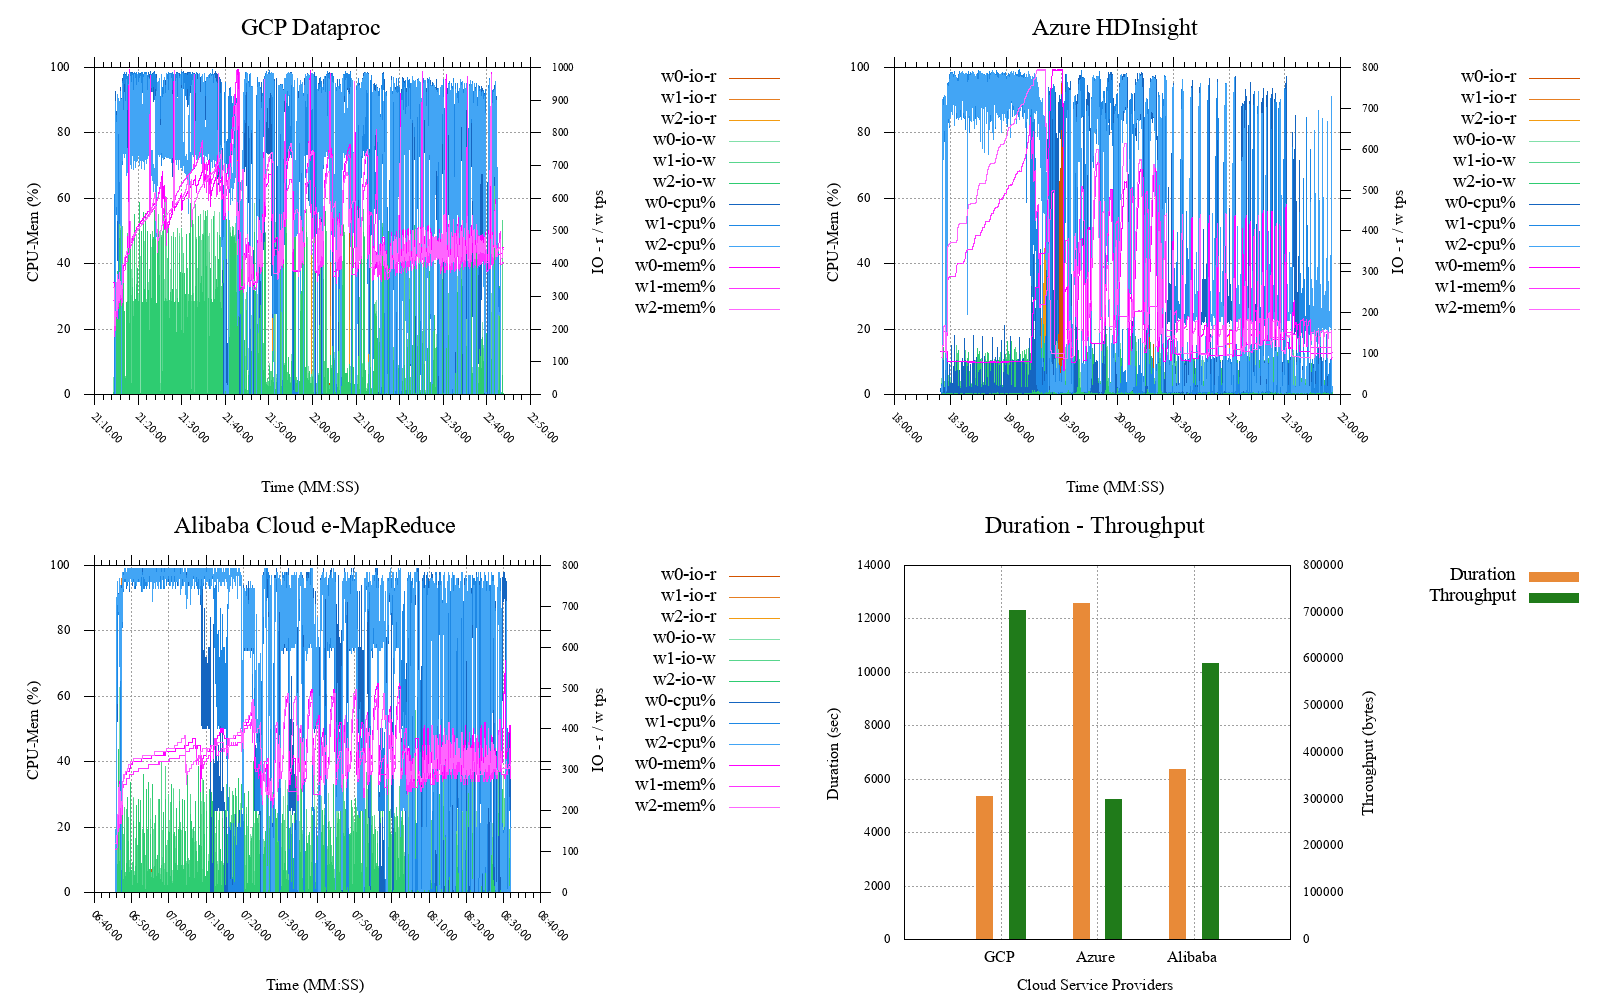
\includegraphics[width=\textwidth]{uc1-bayes-g-cmidt}
	\centering
\end{figure}


\subsection{Kmeans}
GCP's CPU performance resulted in the range of about 60\% to below 100\%, whereas memory utilization was about 60\%s, increasing at the reduce phase, where I/O-write activity also centered at 500 tps. The utilization in Azure was measured as a high CPU behavior of about 80\% and 90\%, a moderate memory consumption attained around 20\% up to below 60\%, and I/O transfers estimated around 40 tps, which emerged as the second shortest duration. Alibaba utilized processor and memory in high levels, including drops in processors on particular worker nodes, with an increased I/O-write transfer in reduce phase reached the highest throughput and the shortest duration as illustrated in Figure \ref{fig:uc1-kmeans-h-cmidt}.

\begin{figure}[p]
	\caption{UC1 - Kmeans (Huge; CLUSTERS: 5 DIMENSIONS: 20 SAMPLES: 100,000,000 SAMP PER INPUT: 20,000,000 MAX IT: 5 K: 10 CONVERGEDIST: 0.5)}
	\label{fig:uc1-kmeans-h-cmidt}
	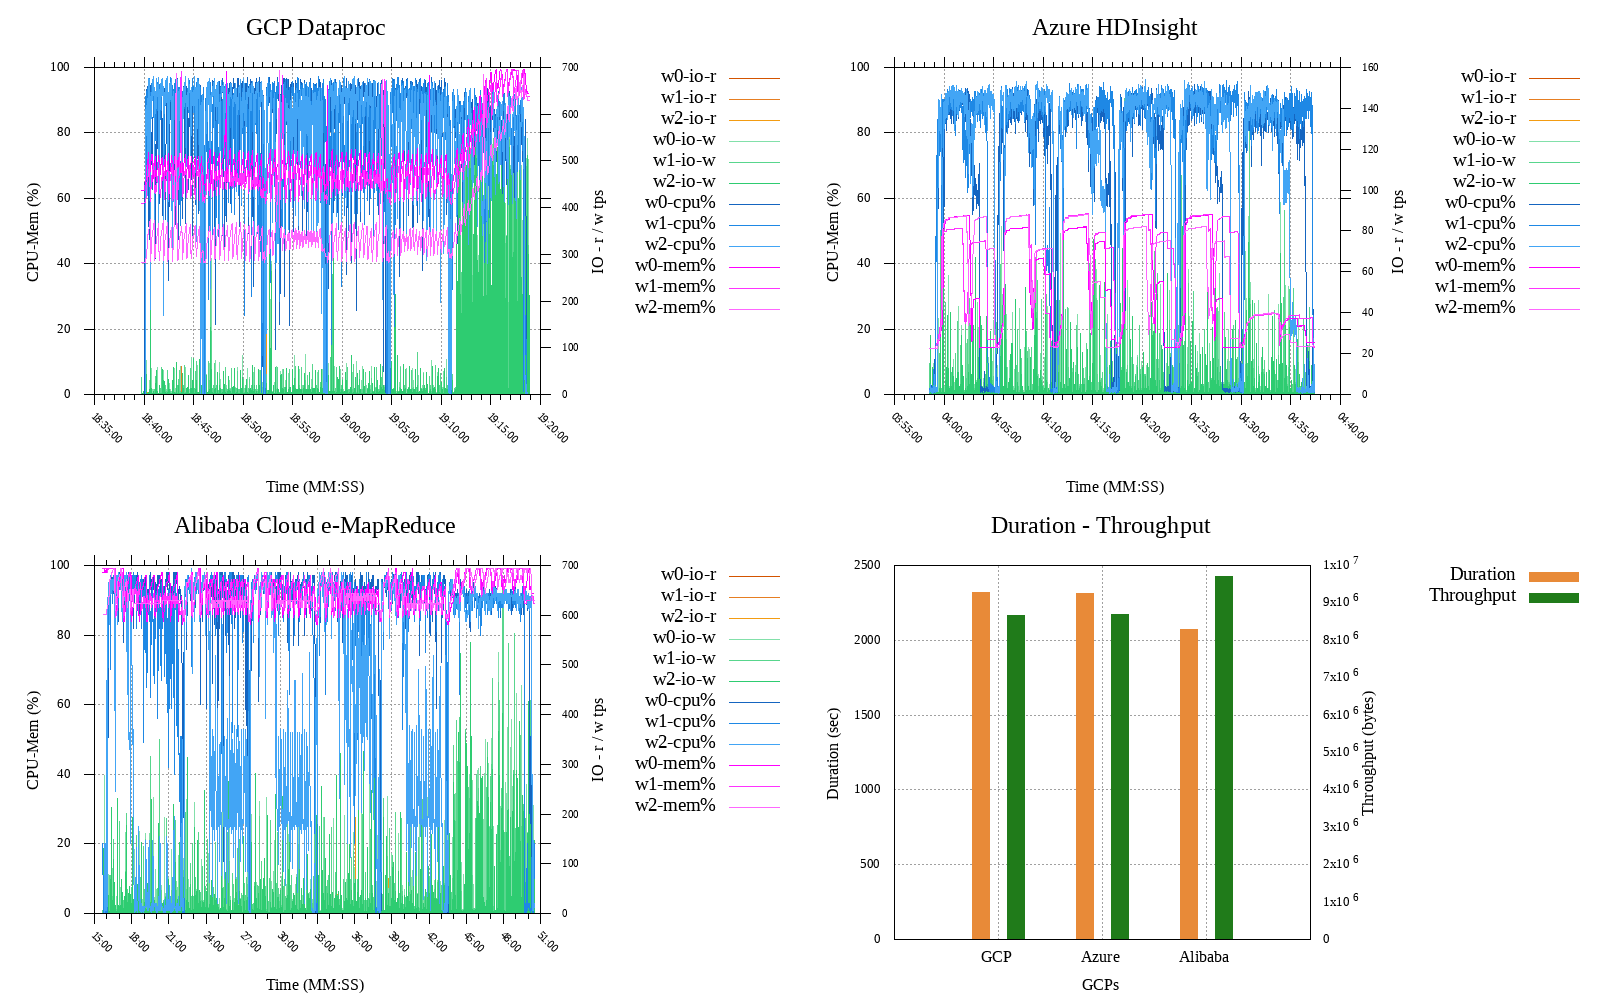
\includegraphics[width=\textwidth]{uc1-kmeans-h-cmidt}
	\centering
\end{figure}

In the gigantic data scale, all three services remained their previous utilization behavior, which is more centered on I/O transfers as observed in Figure \ref{fig:uc1-kmeans-g-cmidt}. The performances of Alibaba and Azure were comparable in throughputs. The resulting outcome was 4034 seconds for Alibaba and 4042 seconds for Azure, GCP's duration did not stand far apart by 4541 seconds.

\begin{figure}[p]
	\caption{UC1 - Kmeans (Gigantic; CLUSTERS: 5 DIMENSIONS: 20 SAMPLES: 200,000,000 SAMP PER INPUT: 40,000,000 MAX IT: 5 K: 10 CONVERGEDIST: 0.5)}
	\label{fig:uc1-kmeans-g-cmidt}
	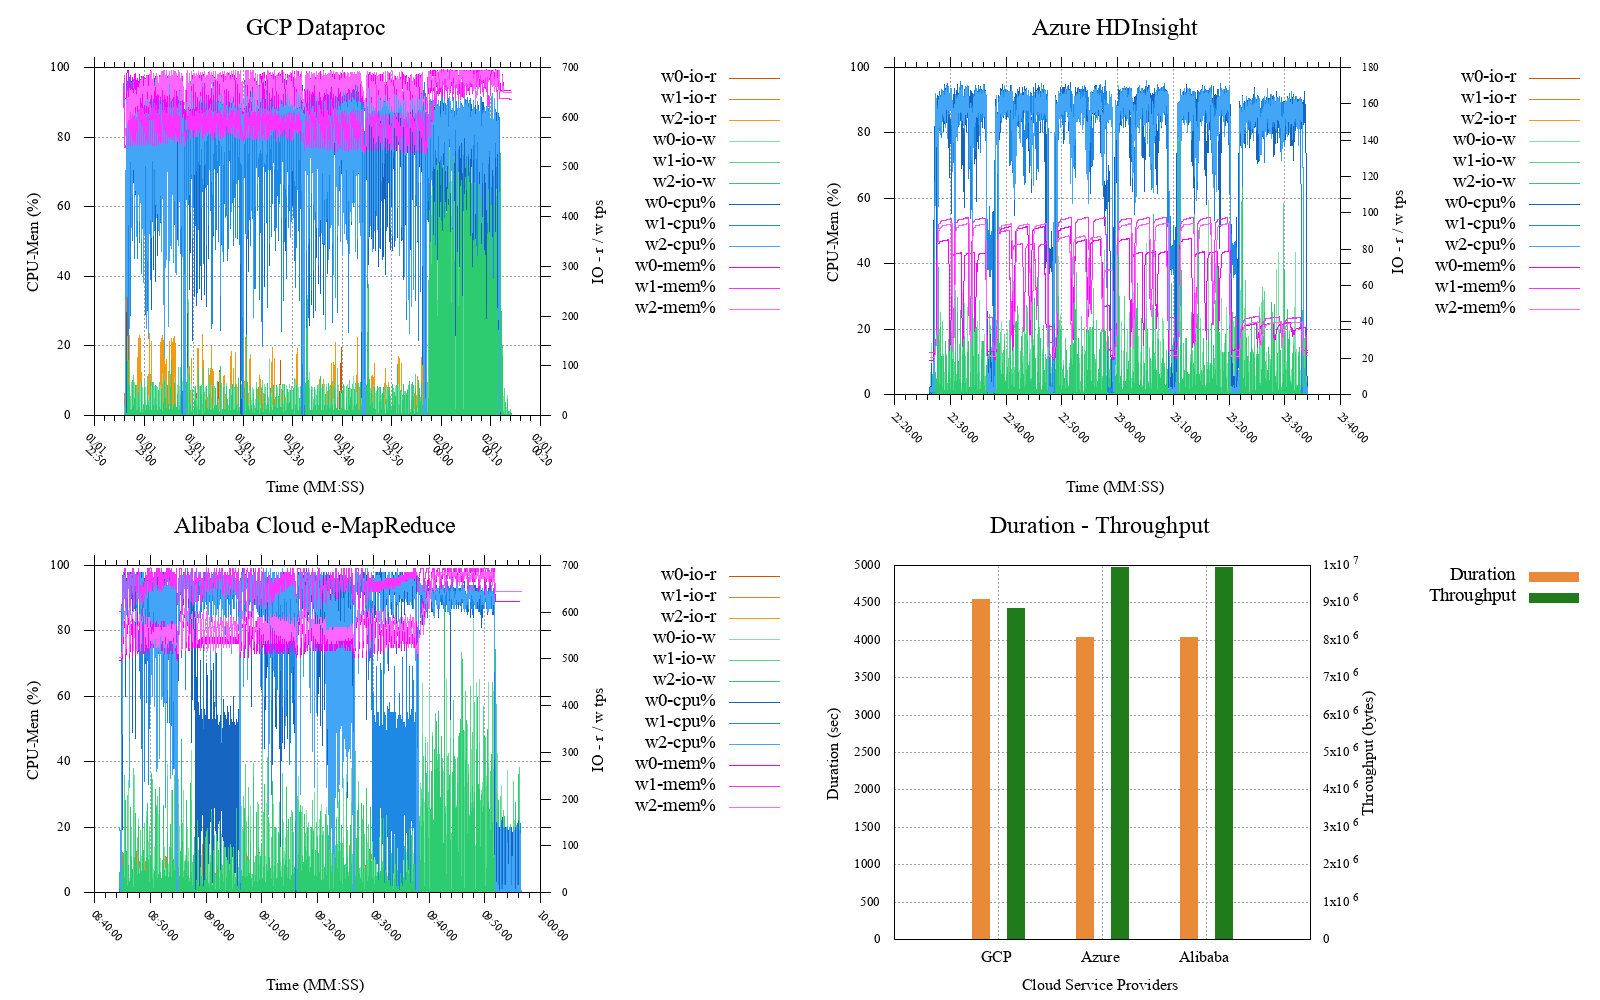
\includegraphics[width=\textwidth]{uc1-kmeans-g-cmidt}
	\centering
\end{figure}


\subsection{Pagerank}
GCP's processor utilization performed in a higher range at about 70\% and below 100\%; RAM utilization was resulted in an intermediate performance moving along to 50\%, including peak points at below 100\%, I/O transfers topped around 500 tps, resulting in the best performance by 1544 seconds as revealed in Figure \ref{fig:uc1-page-h-cmidt}. Azure performed a high utilization behavior in the processor at about 80\% to over 90\%, memory load changed between about 20\% up to 60\%, a lower level range of 100 tps to 150 tps characterizes its I/O transfer utilization resulted in 3334 seconds duration. Alibaba's both CPU and memory utilization across worker nodes were between 80\%s and lower 100\%s, and I/O transfer behavior pushing upper limits at about 600 tps, which reached second-highest throughput resulting in 2458 seconds.
 
\begin{figure}[p]
	\caption{UC1 - Pagerank (Huge; PAGES: 5,000,000 NUM ITERATIONS: 3 BLOCK: 0 BLOCK WIDTH: 16)}
	\label{fig:uc1-page-h-cmidt}
	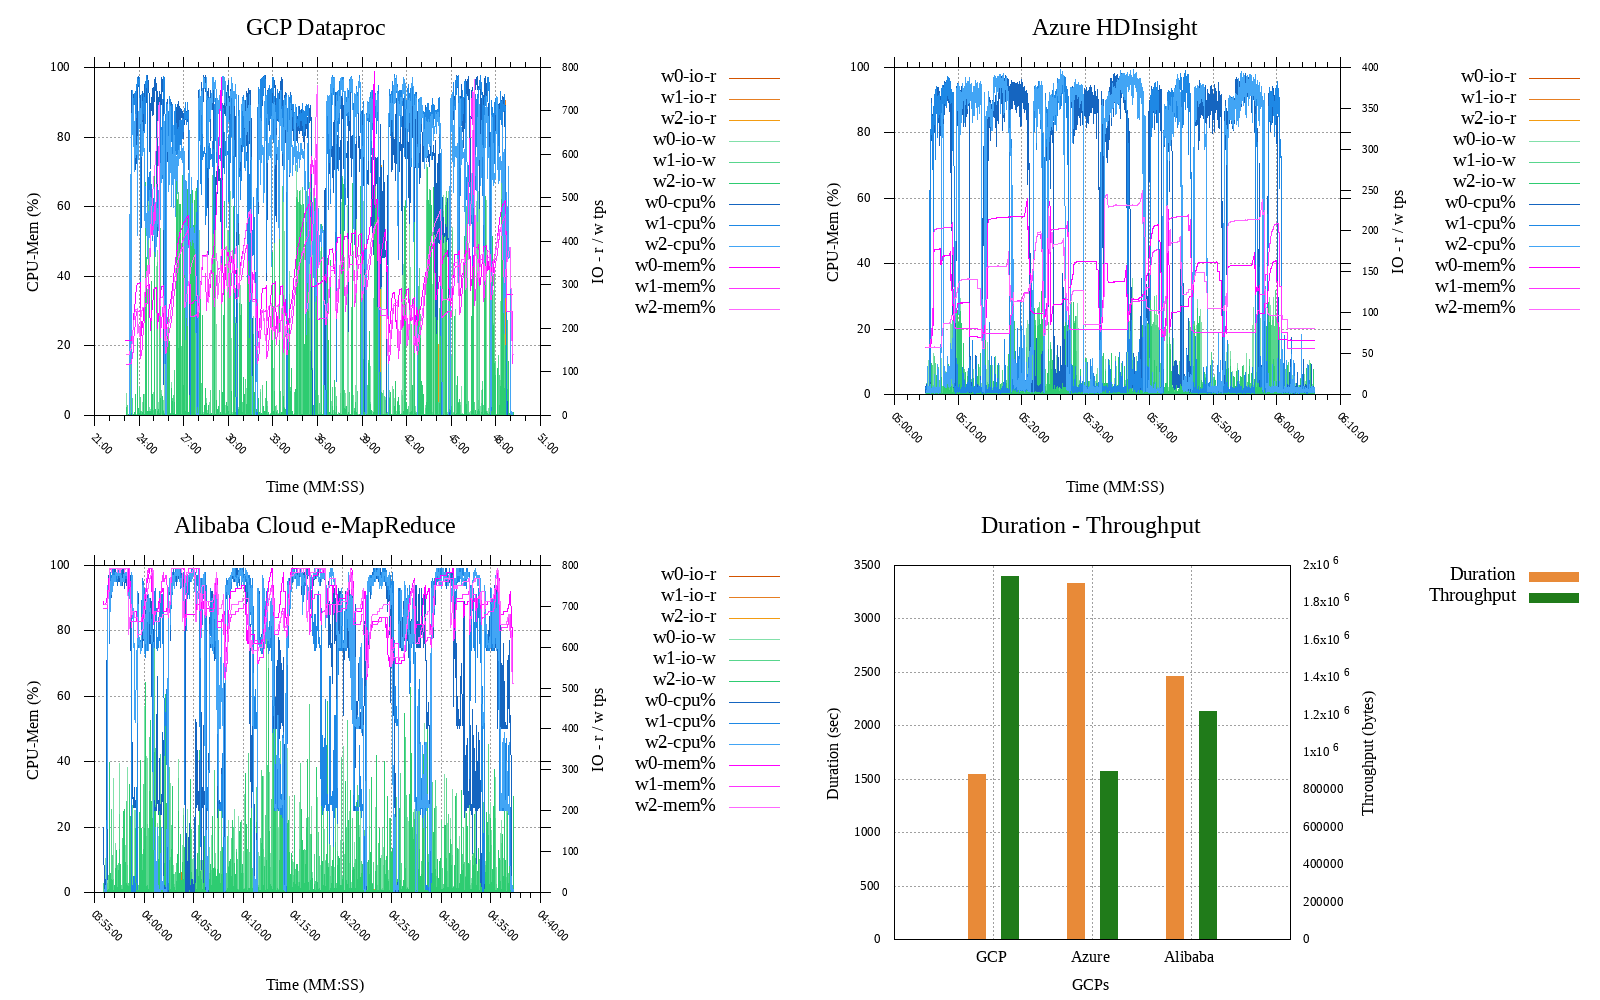
\includegraphics[width=\textwidth]{uc1-page-h-cmidt}
	\centering
\end{figure}

When assessing the benchmark performance in gigantic scale, the CPU load of GCP was measured in a range of about 60\% up to below 100\%, a fluctuating RAM utilization behavior incremented three times to 100\% over the execution time, and an I/O transfer at 500 tps performed the highest throughput and shortest duration of 8,371 seconds as noted in the Figure \ref{fig:uc1-page-g-cmidt}. Azure's processor load varied between 70\%s up to below 100\%, showed fluctuating memory utilization between 40\%s and 100\%, general I/O transfers were limited to about 200 tps with peak exceptions at about 5000 tps performing the second shortest duration of 11,779 seconds. Alibaba's resource utilization remained stable for CPU and memory load; I/O transfers mostly stayed below 300 tps, topped at 600 tps to 1200 tps several times during execution, performing the lowest throughput result in the longest duration of 13,893 seconds.

\begin{figure}[p]
	\caption{UC1 - Pagerank (Gigantic; PAGES: 30,000,000 NUM ITERATIONS: 3 BLOCK: 0 BLOCK WIDTH: 16)}
	\label{fig:uc1-page-g-cmidt}
	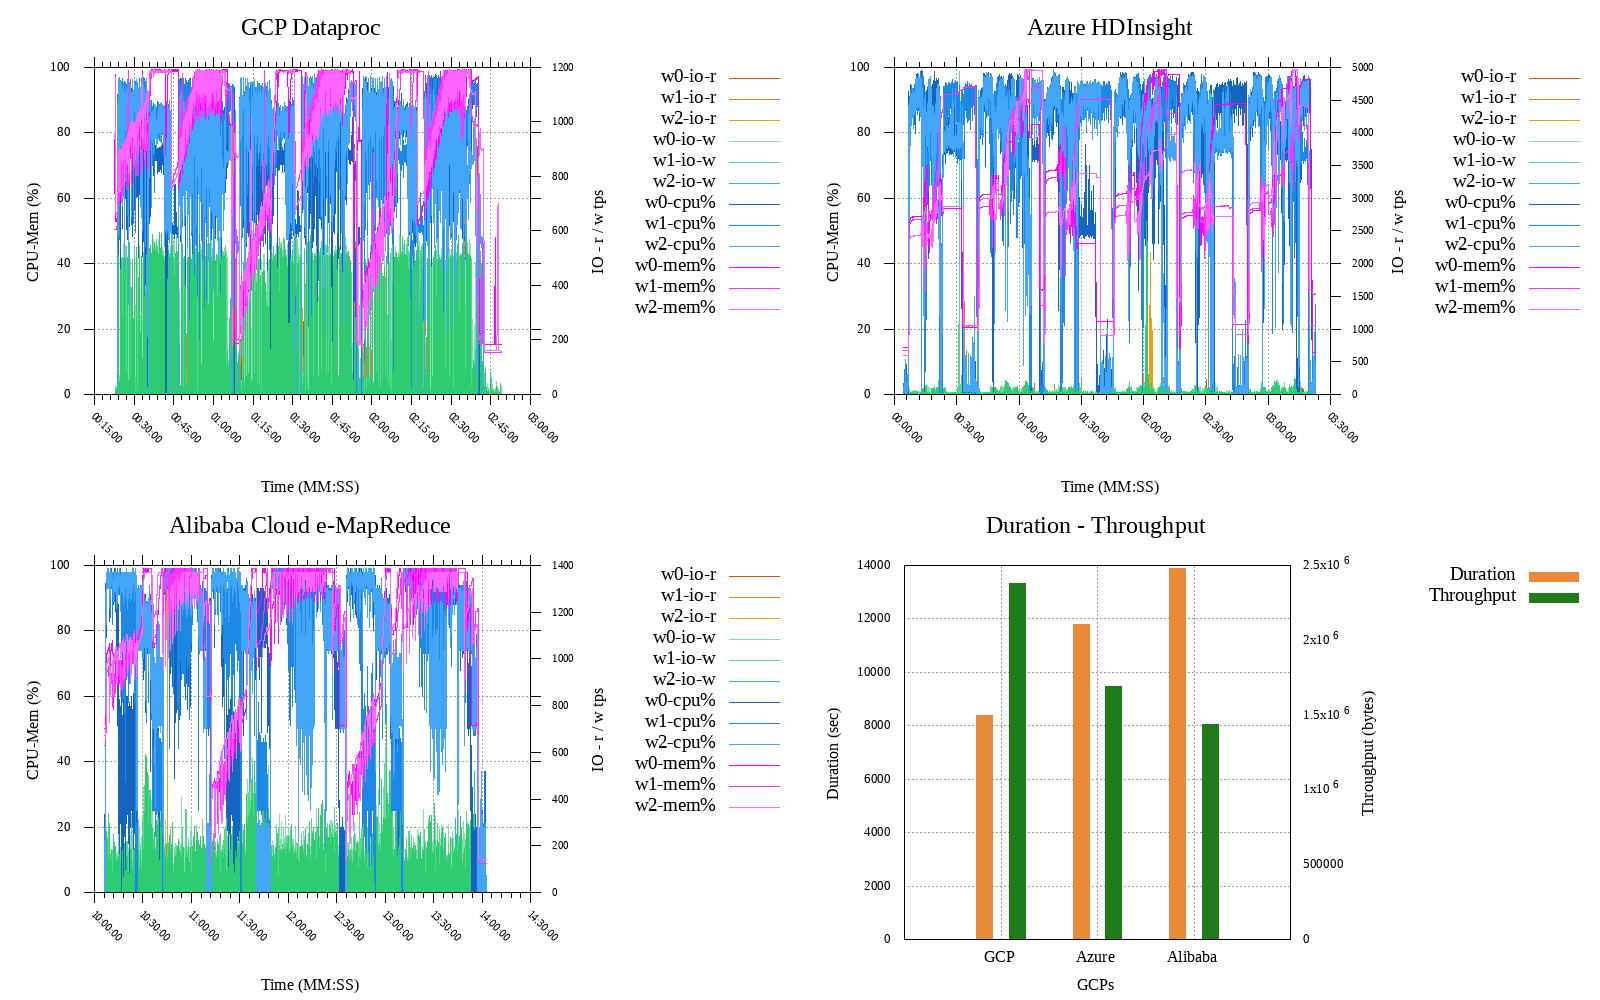
\includegraphics[width=\textwidth]{uc1-page-g-cmidt}
	\centering
\end{figure}



\section{Use Case 2 Results}
In this section, we evaluated the utilization of I/O transfers per second based on Sort benchmark task and the CPU utilization performance using the Wordcount benchmark for each cloud provider. Table \ref{tab:uc2-results} shows the overall results of Use Case 2 evaluations.

%% Use Case 2 Tabular Results:
\begin{table}
	\centering
	\small
	\caption{Use Case 2 benchmark results}
	\label{tab:uc2-results}
	\begin{tabular}[b]{ l r r r r r r r }
		{} & {} & \multicolumn{2}{ c }{\textbf{Dataproc}} & \multicolumn{2}{ c }{\textbf{HDInsight}} & \multicolumn{2}{ c }{\textbf{e-MapReduce}} \\
		\hline
		{Benchmark} & {IDS} & \begin{math}D_{(s)}\end{math} & \begin{math}T_{(MB/s)}\end{math} & \begin{math}D_{(s)}\end{math} & \begin{math}T_{(MB/s)}\end{math} & \begin{math}D_{(s)}\end{math} & \begin{math}{T_{(MB/s)}}\end{math} \\
		\hline
		Sort (t) & 39.30 KB & 36 & 0.0012 & 69 & 0.0006 & 32 & 0.0012 \\
		Sort (s) & 3.28 MB & 36 & 0.09 & 70 & 0.0471 & 31 & 0.105 \\
		Sort (l) & 328.50 MB & 42 & 7.86 & 81 & 4.07 & 42 & 7.74 \\
		Sort (h) & 3.28 GB & 70 & 47.08 & 141 & 23.36 & 107 & 30.69 \\
		Sort (g) & 32.85 GB & 694 & 47.30 & 699 & 47.00 & 883 & 37.20 \\
		Wordcount(t) & 38.65 KB & 38 & 0.001 & 68 & 0.0006 & 31 & 0.0012 \\
		Wordcount (s) & 348.29 MB & 50 & 6.51 & 98 & 3.34 & 47 & 7.06 \\
		Wordcount (l) & 3.28 GB & 129 & 25.45 & 269 & 12.20 & 120 & 27.27 \\
		Wordcount (h) & 32.85 GB & 952 & 34.51 & 1487 & 22.10 & 888 & 37.00 \\
		Wordcount (g) & 328.49 GB & 9749 & 33.70 & 13286 & 24.73 & 8622 & 38.10 \\
		\hline
		\multicolumn{8}{r}{IDS: Input Data Size; \begin{math}D_{(s)}\end{math}: duration (sec); \begin{math}T_{(MB/s)}\end{math}: throughput (MB/sec)} \\
		\multicolumn{8}{ r }{(t): tiny, (s): small, (l): large, (h): huge, (g): gigantic} \\
		\hline
	\end{tabular}
\end{table}

%Serkan: overview kısmını sondan başa taşıdım

In the evaluations of Sort and Wordcount benchmarks, we assessed the scalability performances of the cloud providers using data scales Tiny, Small, Large, Huge, and Gigantic in respective order. The spider plot visualizations were used for illustration of the results. Figure \ref{fig:uc2-srt-new} and Figure \ref{fig:uc2-wrdcnt-new} show the utilization averages per cluster in the axes. The performances depicted in Sort benchmark indicated that Azure performed significantly less than its counterparts in Tiny, Small, Large, and Huge data scales, yet its performance in the gigantic data scale was improved. In the Wordcount benchmark, where high CPU utilization among the services likely to have occurred, the compressed I/O average load was the determining aspect of higher throughput and better performance for Alibaba.

\begin{figure}[p]
	\caption{Use Case 2 - Sort performances along with data scales}
	\label{fig:uc2-srt-new}
	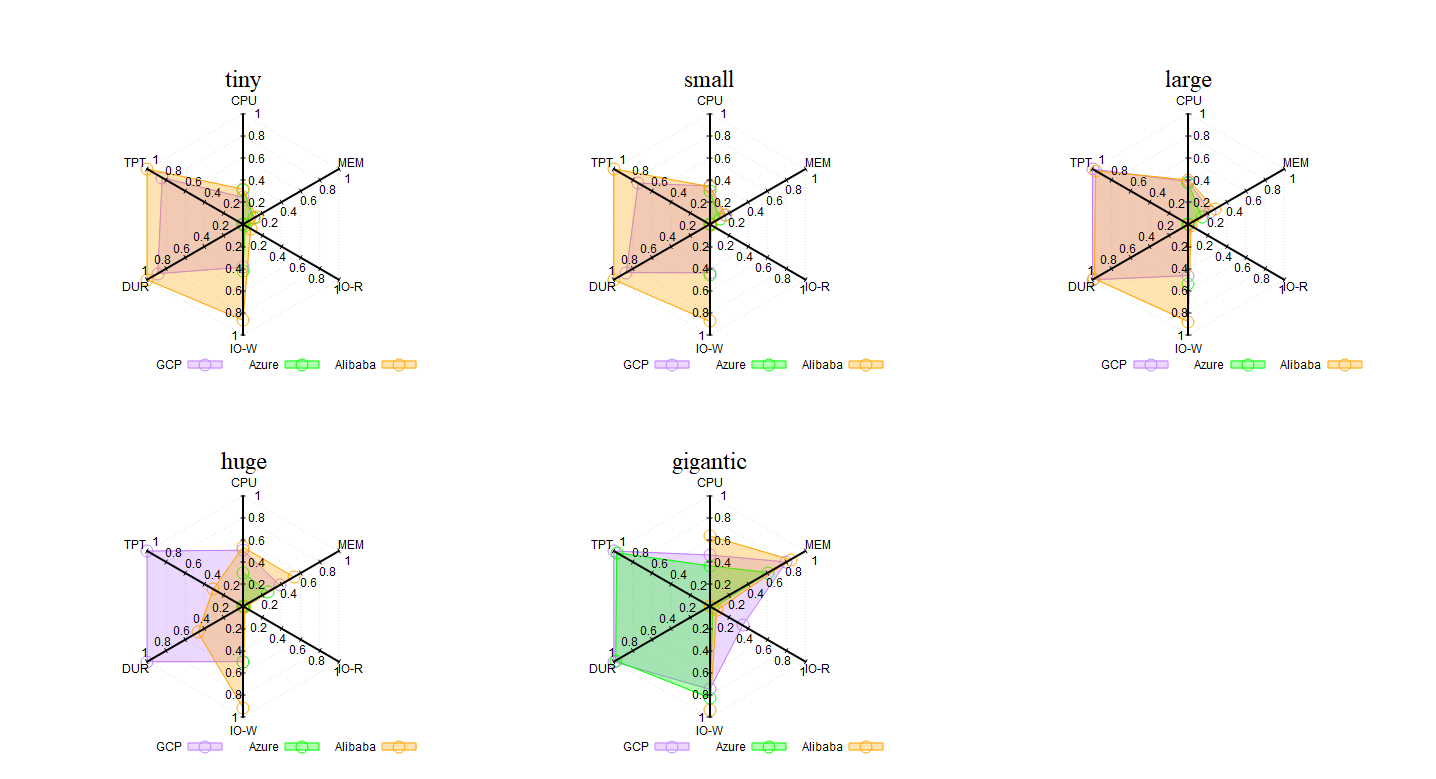
\includegraphics[width=\textwidth]{uc2-srt-new}
	\centering
\end{figure}

\begin{figure}[p]
	\caption{Use Case 2 - Wordcount performances along with data scales}
	\label{fig:uc2-wrdcnt-new}
	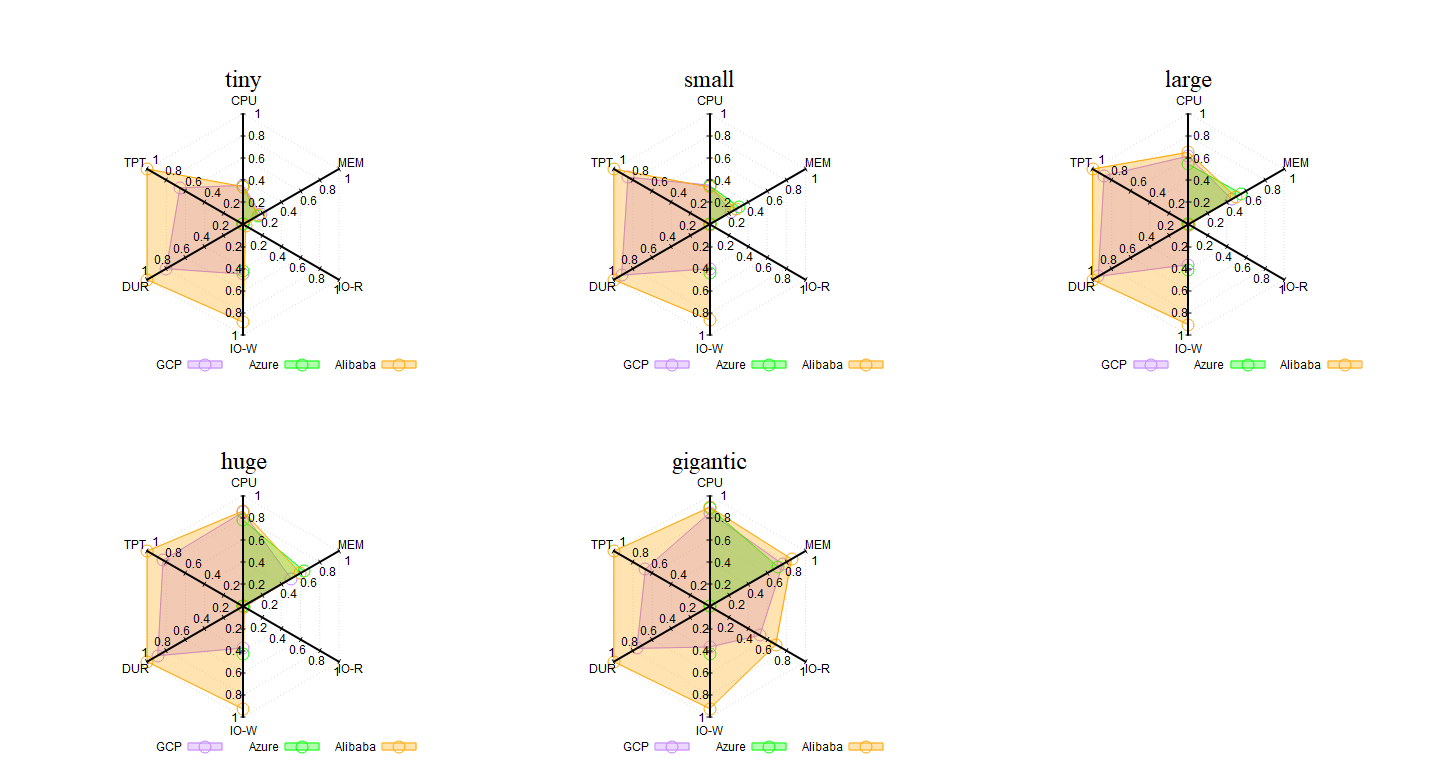
\includegraphics[width=\textwidth]{uc2-wrdcnt-new}
	\centering
\end{figure}


\subsection{Scalability Results in Sort Benchmark}
In the data scales tiny and small, I/O transfers of the managed systems remained within similar boundaries, reaching peak points at about 80 tps for GCP, 30 tps to 35 tps for Azure, and about 200 tps for Alibaba, reaching the highest throughput thus shortest duration in lighter data scales as shown in Figures \ref{fig:uc2-srt-t-cmidt} and \ref{fig:uc2-srt-s-cmidt}. 

\begin{figure}[p]
	\caption{UC2 - Sort (Tiny; 32 KB)}
	\label{fig:uc2-srt-t-cmidt}
	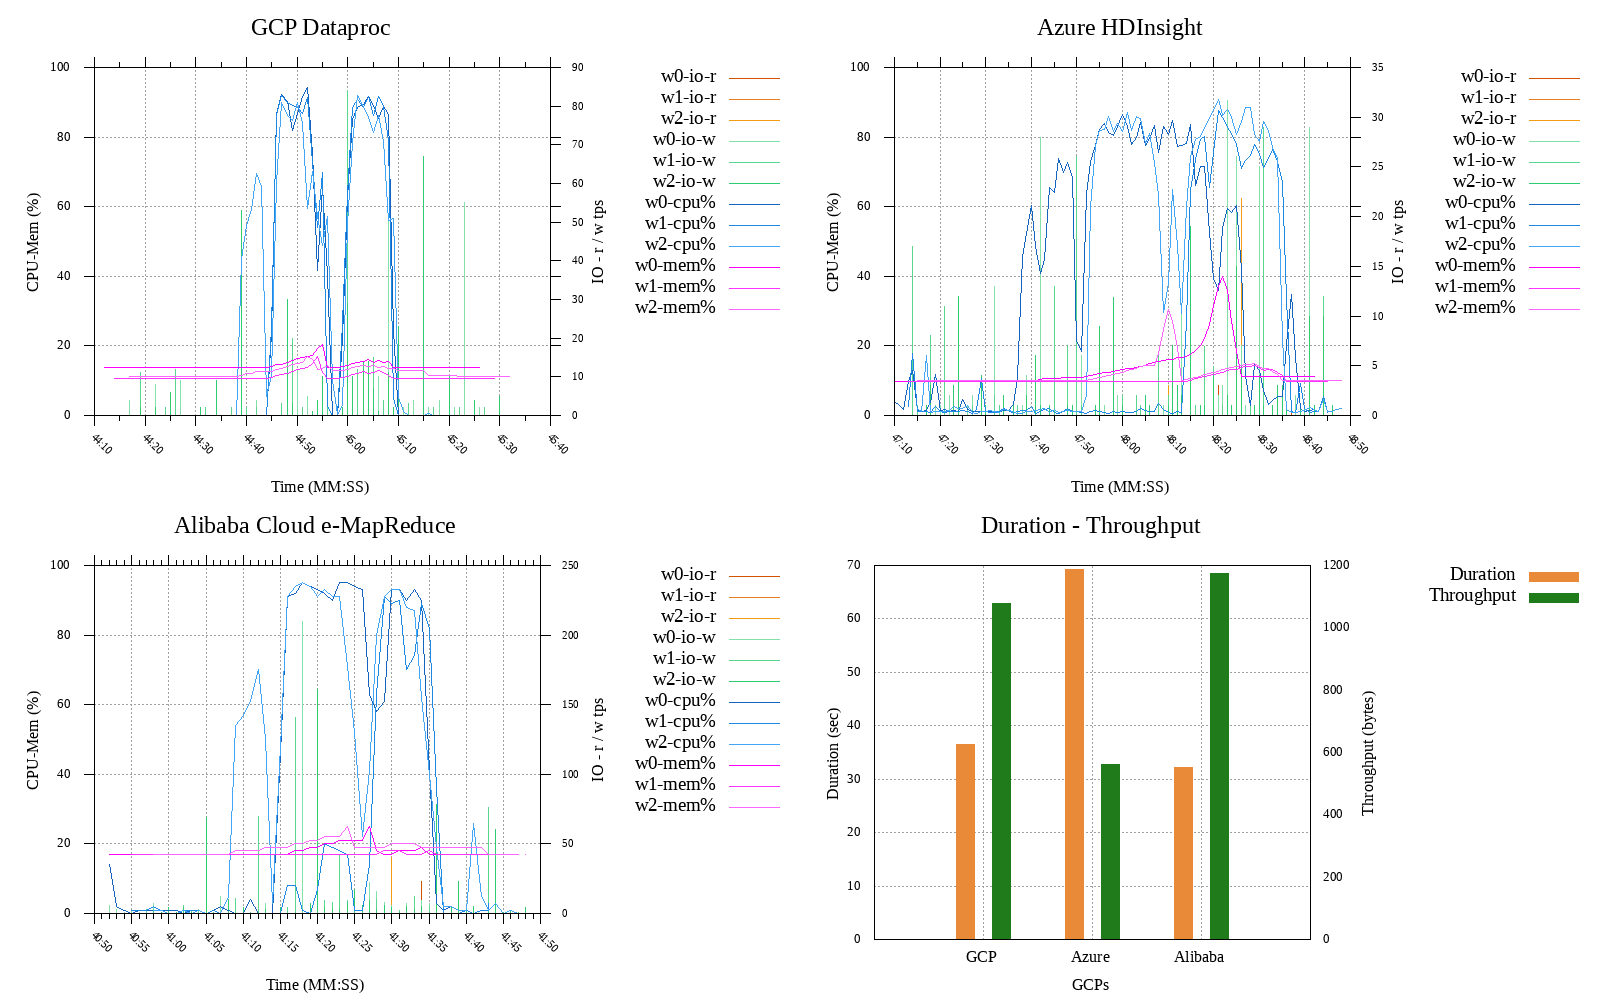
\includegraphics[width=\textwidth]{uc2-srt-t-cmidt}
	\centering
\end{figure}

\begin{figure}[p]
	\caption{UC2 - Sort (Small; 3.2 MB)}
	\label{fig:uc2-srt-s-cmidt}
	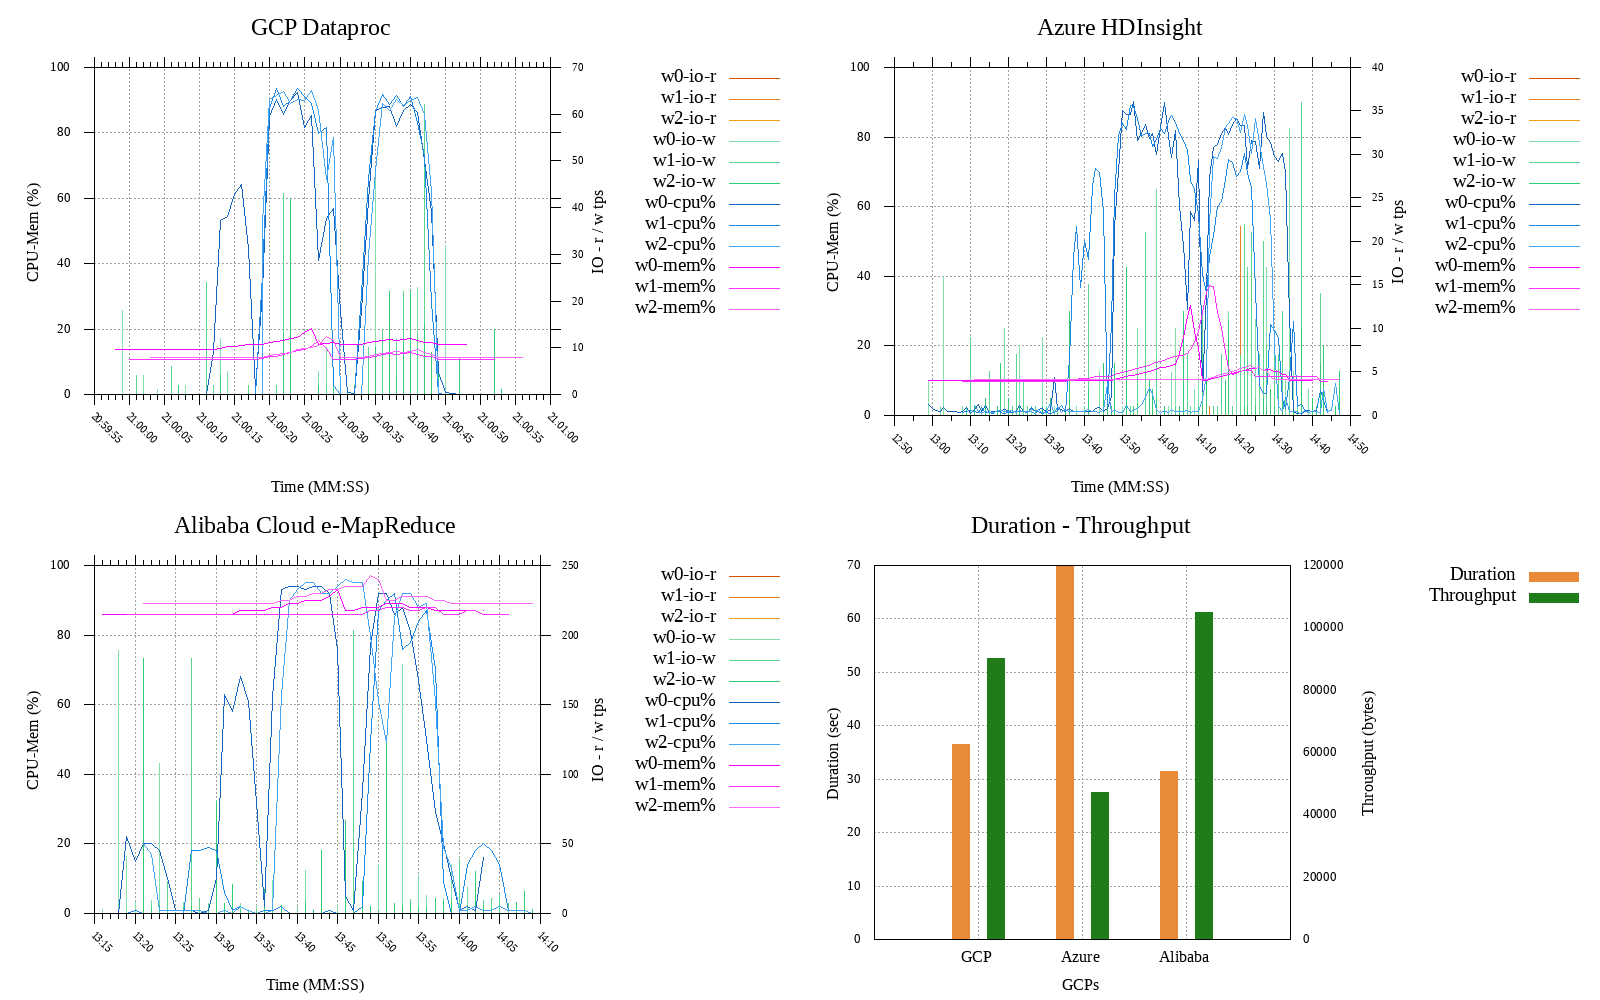
\includegraphics[width=\textwidth]{uc2-srt-s-cmidt}
	\centering
\end{figure}

At 328.5 MB input data size, which corresponds to the large data scale, GCP and Alibaba performed with an equal duration of 42 seconds, GCP utilized I/O peaking at about 110 tps, whereas Alibaba scored its top at 189 tps. Azure's I/O utilization peaked at about 80 tps and a duration of 81 seconds as demonstrated in Figure \ref{fig:uc2-srt-l-cmidt}. 

\begin{figure}[p]
	\caption{UC2 - Sort (Large; 320 MB)}
	\label{fig:uc2-srt-l-cmidt}
	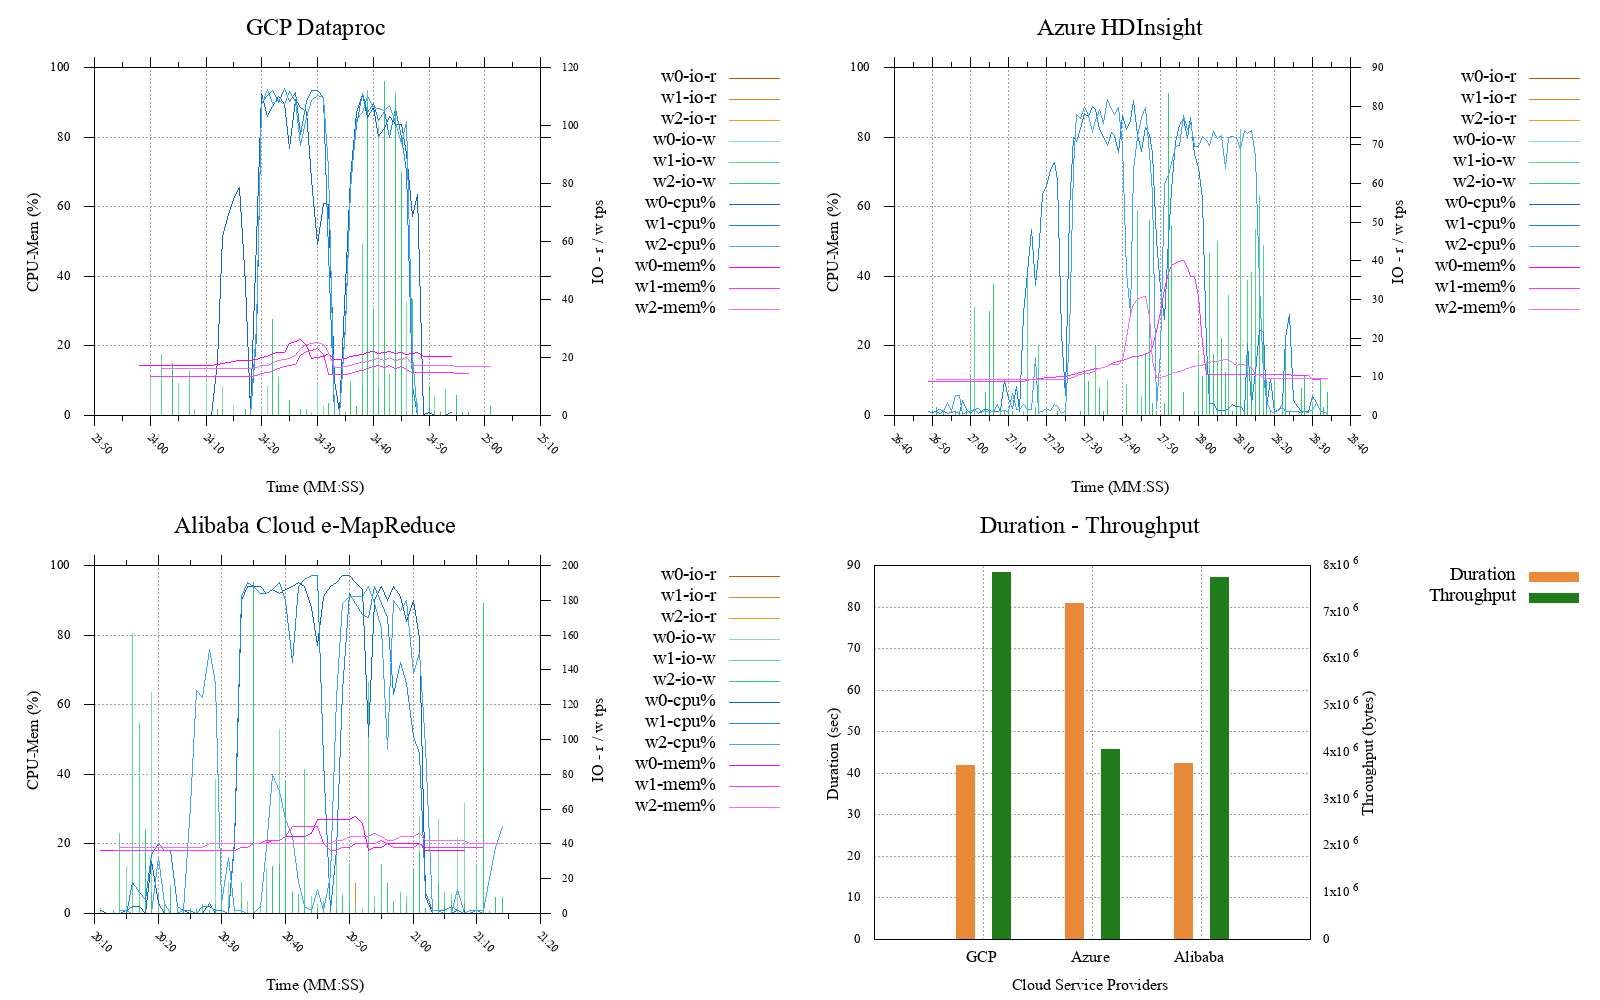
\includegraphics[width=\textwidth]{uc2-srt-l-cmidt}
	\centering
\end{figure}

%paragraf tekrar olmuş
%In the huge data scale with 3.28 GB data, GCP starts utilizing I/O at instances with about 500 tps, thus performing the highest throughput projected in 70 seconds. Azure shows a condensed I/O transfer load at around 80 tps, peaking at 140 tps, and results in 140 seconds. 

Figure \ref{fig:uc2-srt-h-cmidt} presents the evaluation results of Sort benchmark with huge data scale using 3.2 GB dataset. GCP's I/O transfers pushed the upper limits at about 500 tps in the reduce phase, thus performing ~47 MB/s throughput and a duration of 70 seconds. Azure's I/O load performed around 80 tps with its peak at 140 tps, and resulted in ~23 MB/s throughput and 141 seconds duration. Alibaba's I/O load varied at about 100 tps to 450 tps, approximately 31 MB/s throughput with 107 seconds response time. 

\begin{figure}[p]
	\caption{UC2 - Sort (Huge; 3.2 GB)}
	\label{fig:uc2-srt-h-cmidt}
	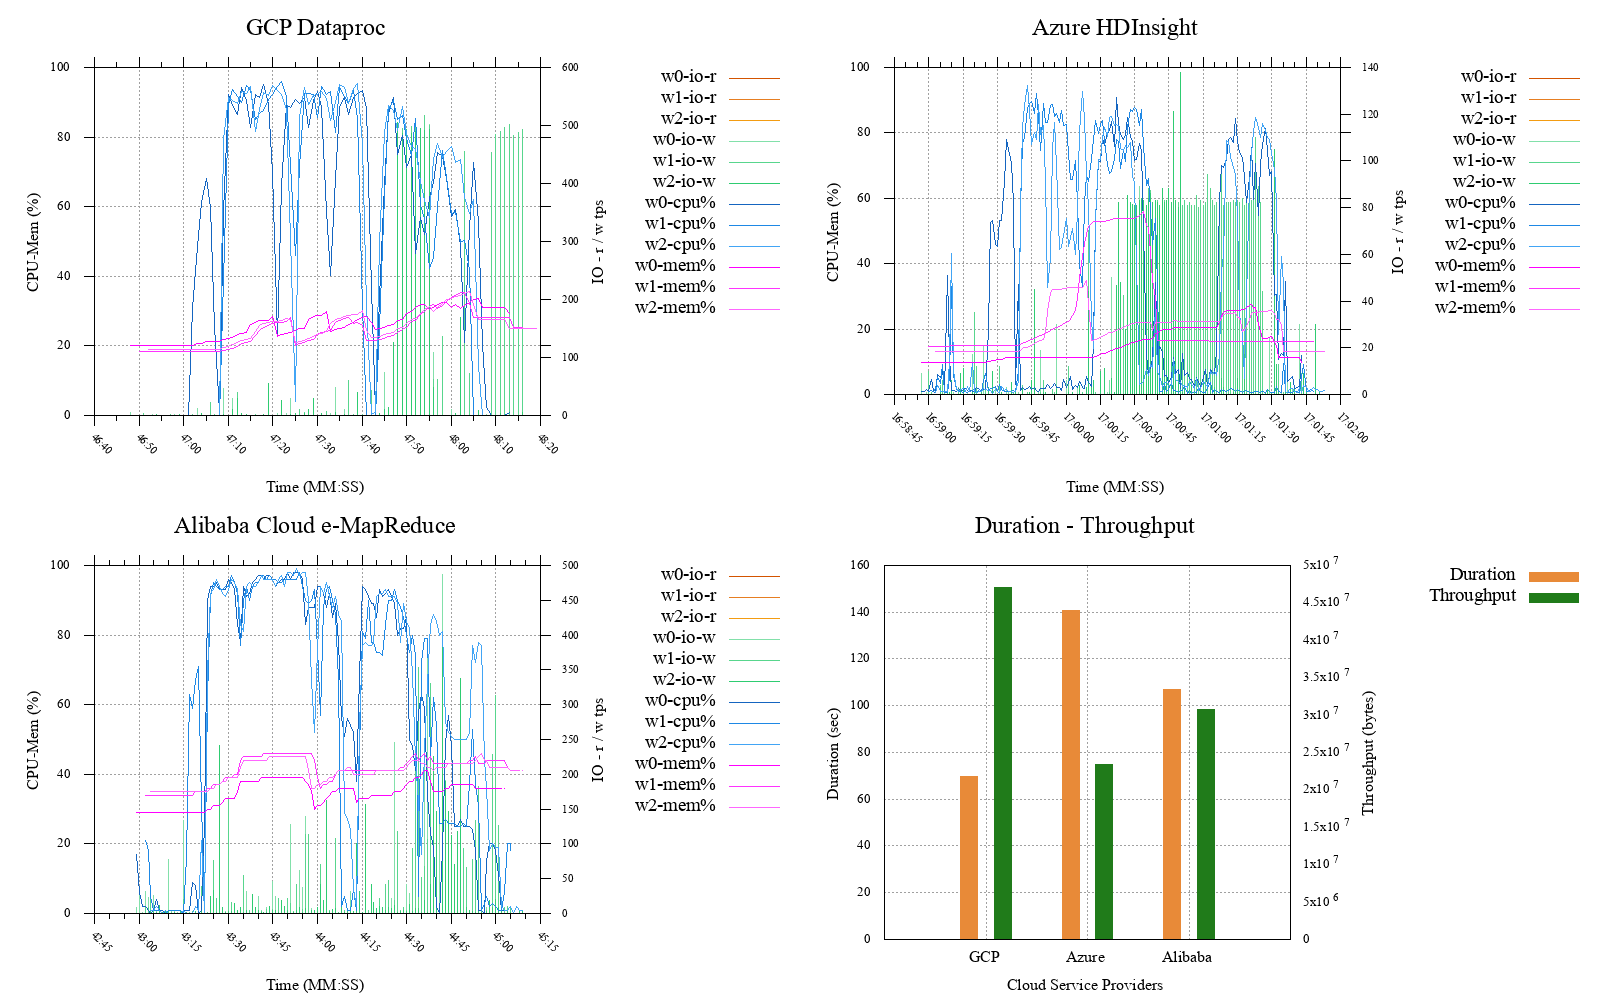
\includegraphics[width=\textwidth]{uc2-srt-h-cmidt}
	\centering
\end{figure}

In the gigantic data scale with an input size of ~32 GB, GCP performed at the level of 500 tps in I/O-reads. Its peak was measured at 1000 tps, with nearly 47 MB/s throughput and 694 seconds of response time. At this scale, Azure improved its performance greatly, even though I/O utilization remained between about 75 tps to 150 tps, carried out a throughput of ~47 MB/s, slightly less than GCP, which resulted in a close follower of the best performance duration, by 699 seconds. Alibaba's I/O activity reached a peak at about 800 tps and changed 400 to 500 tps in reduce phase, and ~37MB/s throughput that resulted in 883 seconds response time as depicted in Figure \ref{fig:uc2-srt-g-cmidt}.

\begin{figure}[p]
	\caption{UC2 - Sort (Gigantic; 32 GB)}
	\label{fig:uc2-srt-g-cmidt}
	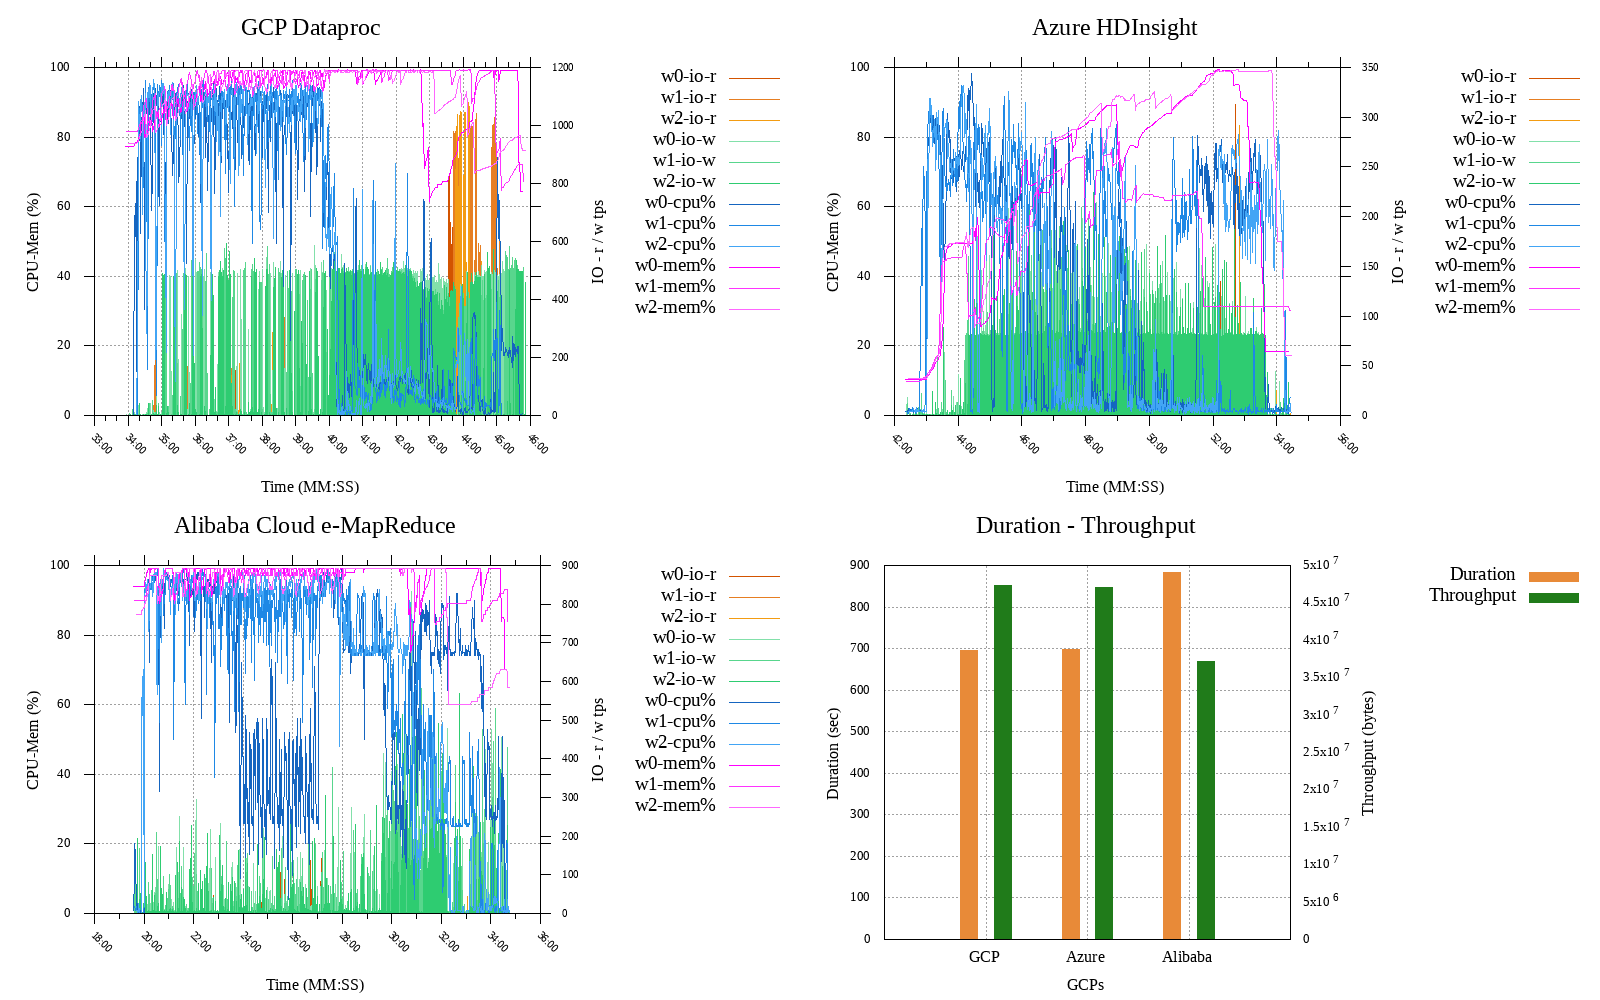
\includegraphics[width=\textwidth]{uc2-srt-g-cmidt}
	\centering
\end{figure}


\subsection{Scalability Results of Wordcount Benchmark}
Following the system utilization of the managed systems along with the plot sequence, the high CPU load of Wordcount was noticeable. More condensed CPU load values were detected in longer duration values. The CPU utilization changes across different managed services were observed within the range of 80\%s and 100\%. However, in Azure, one worker node's CPU load somewhat stayed in a very low range in the data scales Tiny, Small, and Large, which can be seen in Figures \ref{fig:uc2-wrdcnt-t-cmidt}, \ref{fig:uc2-wrdcnt-s-cmidt}, \ref{fig:uc2-wrdcnt-l-cmidt}, respectively. 
Low and mid-level memory consumption across CSPs remained similar between CSPs. In I/O, Alibaba depicts a higher level of transfers per second than its conjugates, which yielded the highest throughput hence the shortest response times for e-MapReduce in all given data scales as demonstrated in Figures \ref{fig:uc2-wrdcnt-h-cmidt}, \ref{fig:uc2-wrdcnt-g-cmidt}.

\begin{figure}[p]
	\caption{UC2 - Wordcount (Tiny; 32 KB)}
	\label{fig:uc2-wrdcnt-t-cmidt}
	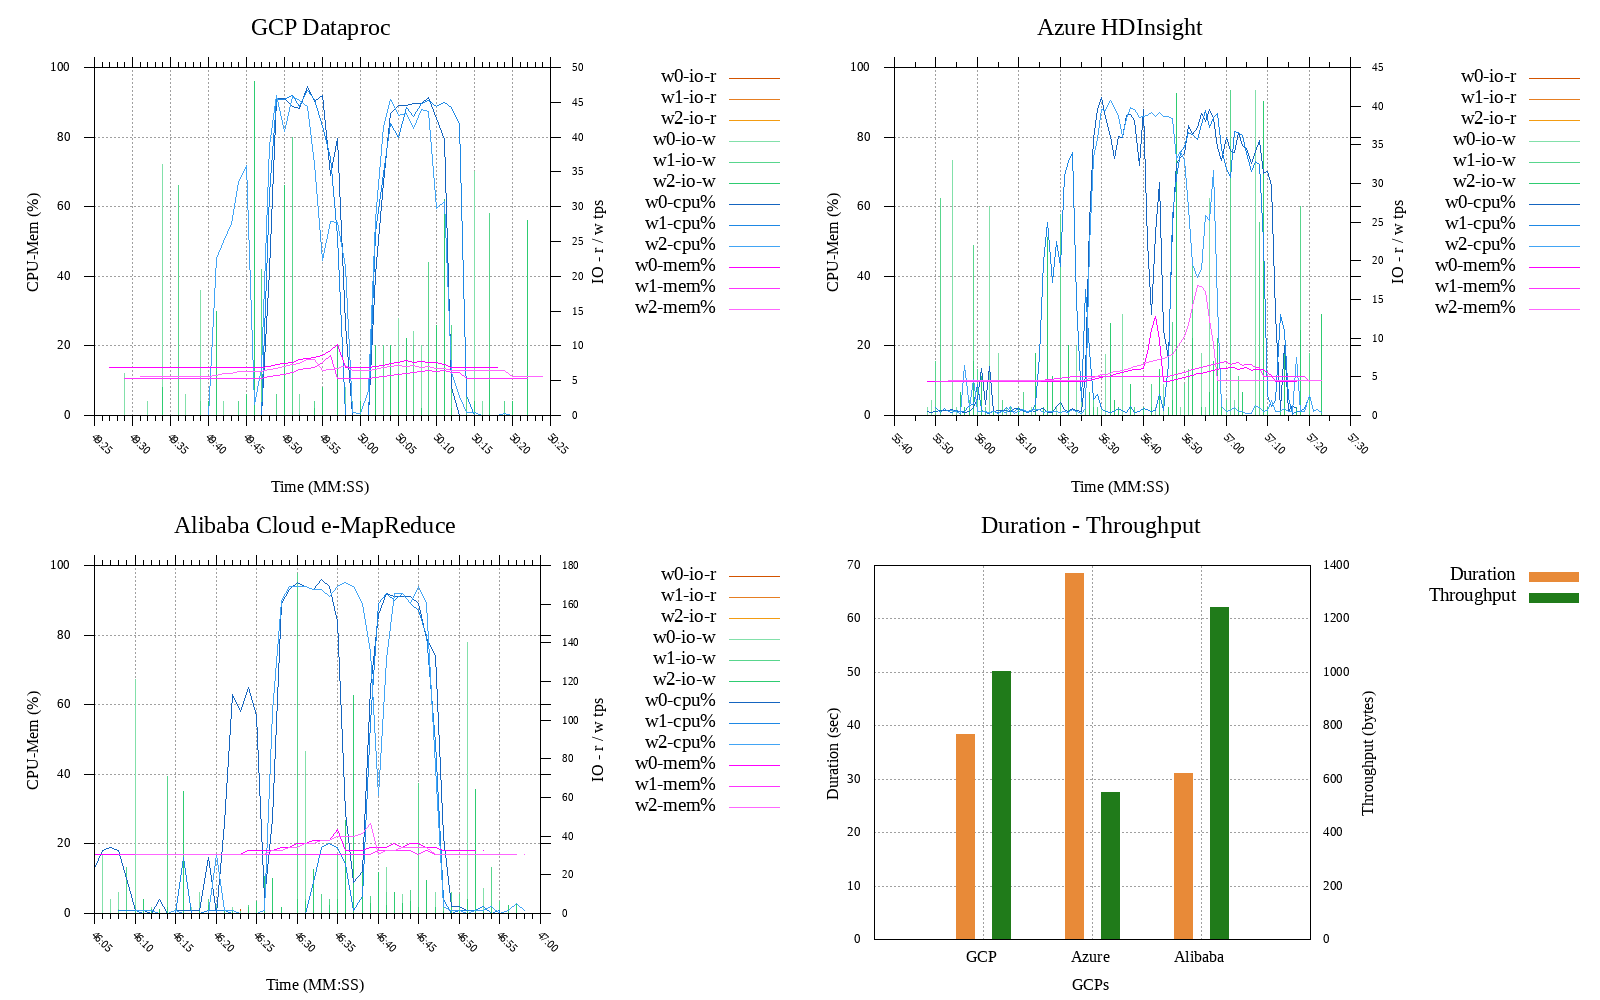
\includegraphics[width=\textwidth]{uc2-wrdcnt-t-cmidt}
	\centering
\end{figure}

\begin{figure}[p]
	\caption{UC2 - Wordcount (Small; 320 MB)}
	\label{fig:uc2-wrdcnt-s-cmidt}
	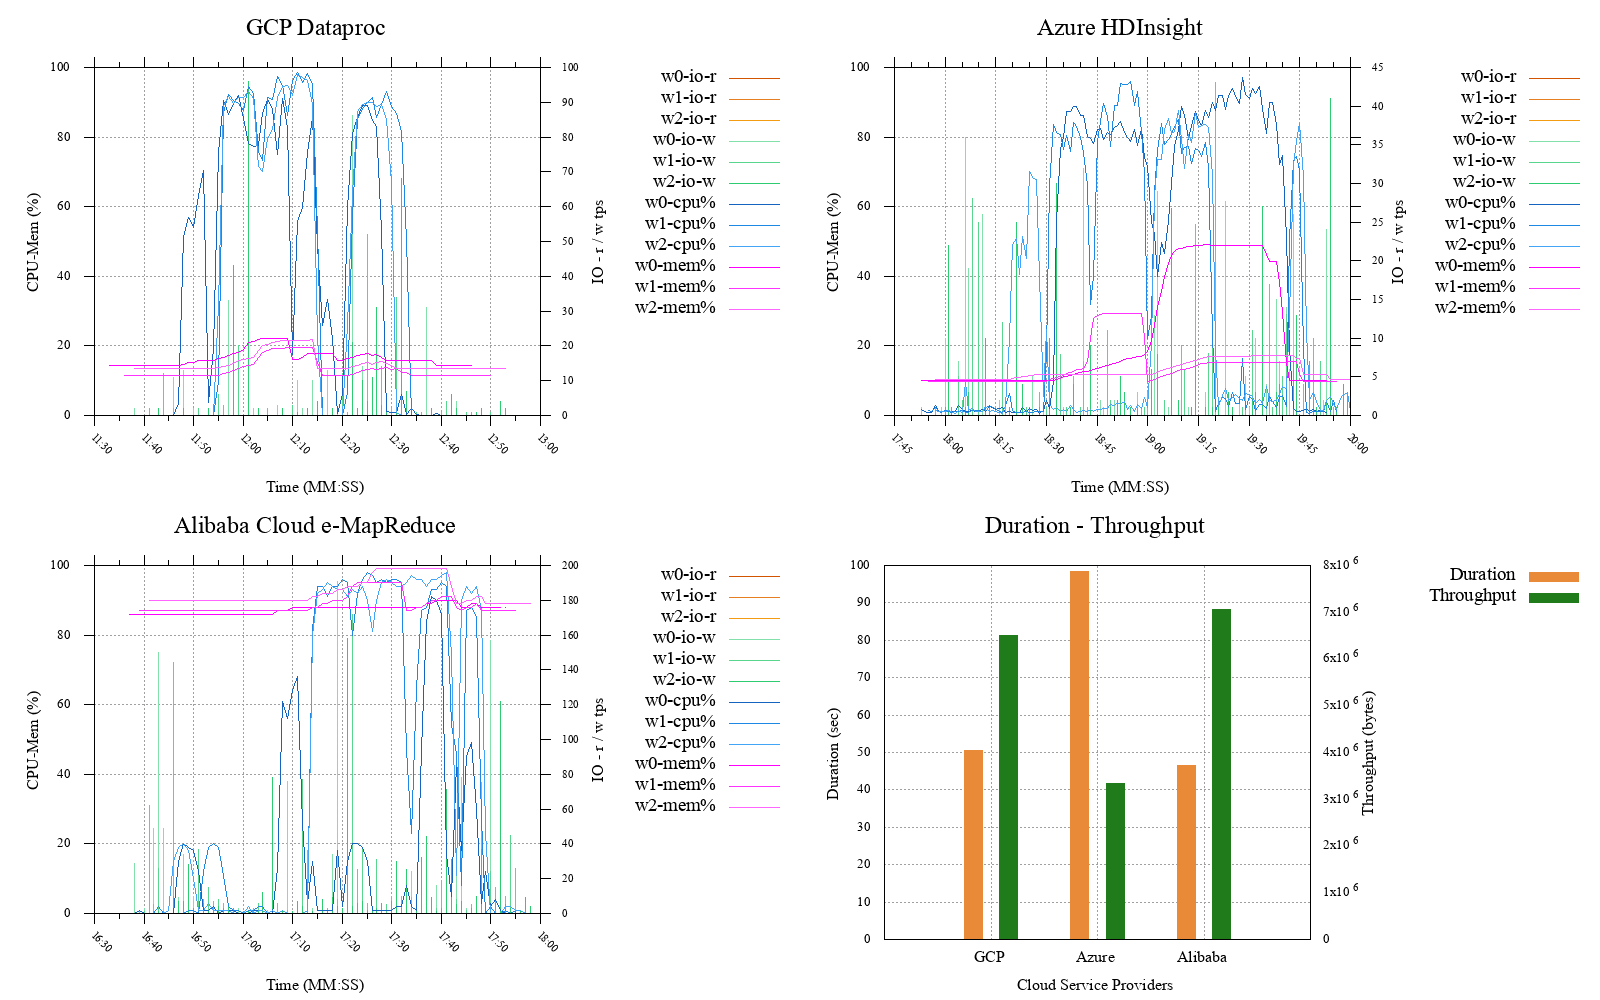
\includegraphics[width=\textwidth]{uc2-wrdcnt-s-cmidt}
	\centering
\end{figure}

\begin{figure}[p]
	\caption{UC2 - Wordcount (Large; 3.2 GB)}
	\label{fig:uc2-wrdcnt-l-cmidt}
	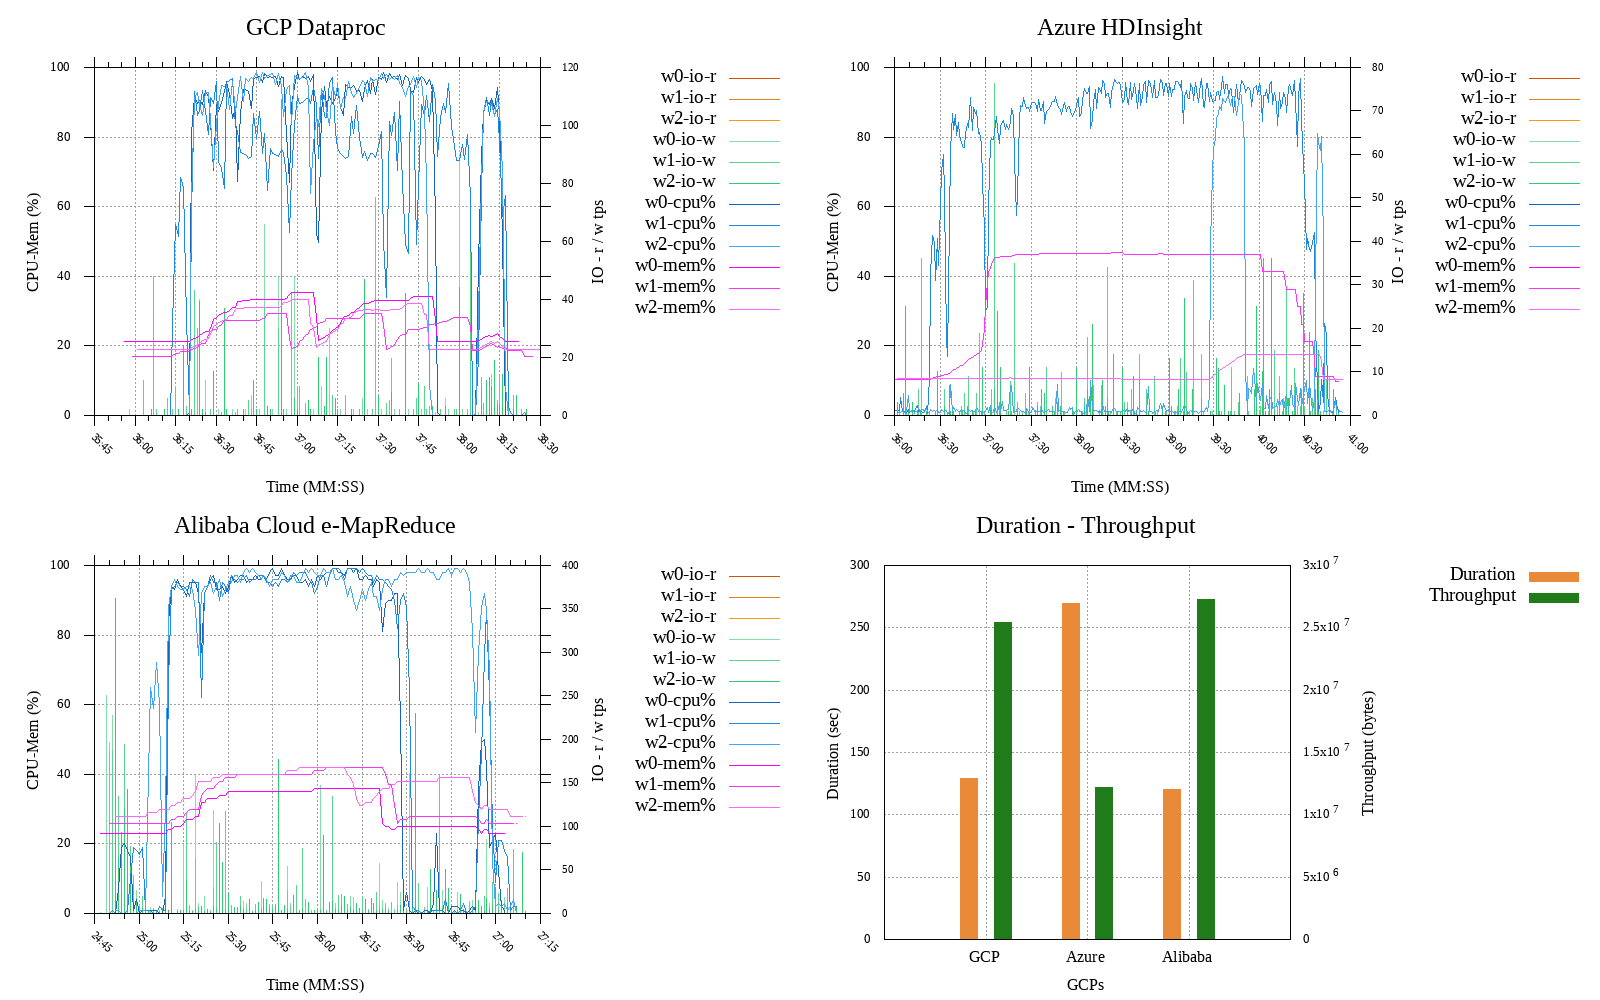
\includegraphics[width=\textwidth]{uc2-wrdcnt-l-cmidt}
	\centering
\end{figure}

\begin{figure}[p]
	\caption{UC2 - Wordcount (Huge; 32 GB)}
	\label{fig:uc2-wrdcnt-h-cmidt}
	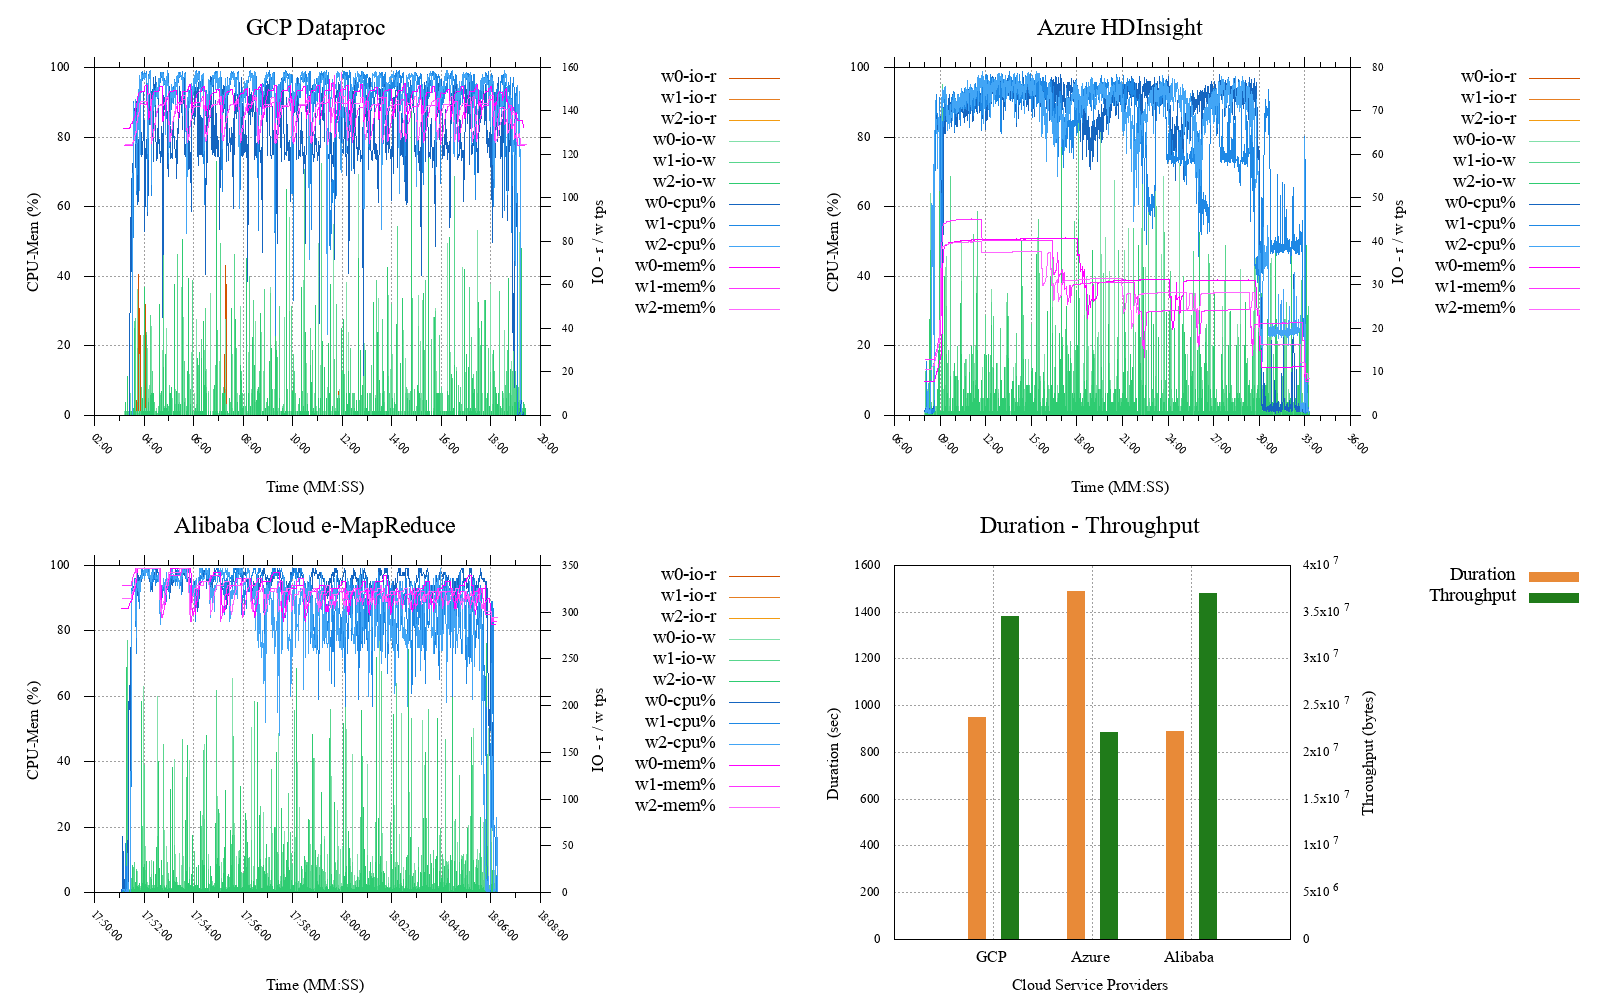
\includegraphics[width=\textwidth]{uc2-wrdcnt-h-cmidt}
	\centering
\end{figure}

\begin{figure}[p]
	\caption{UC2 - Wordcount (Gigantic; 320 GB)}
	\label{fig:uc2-wrdcnt-g-cmidt}
	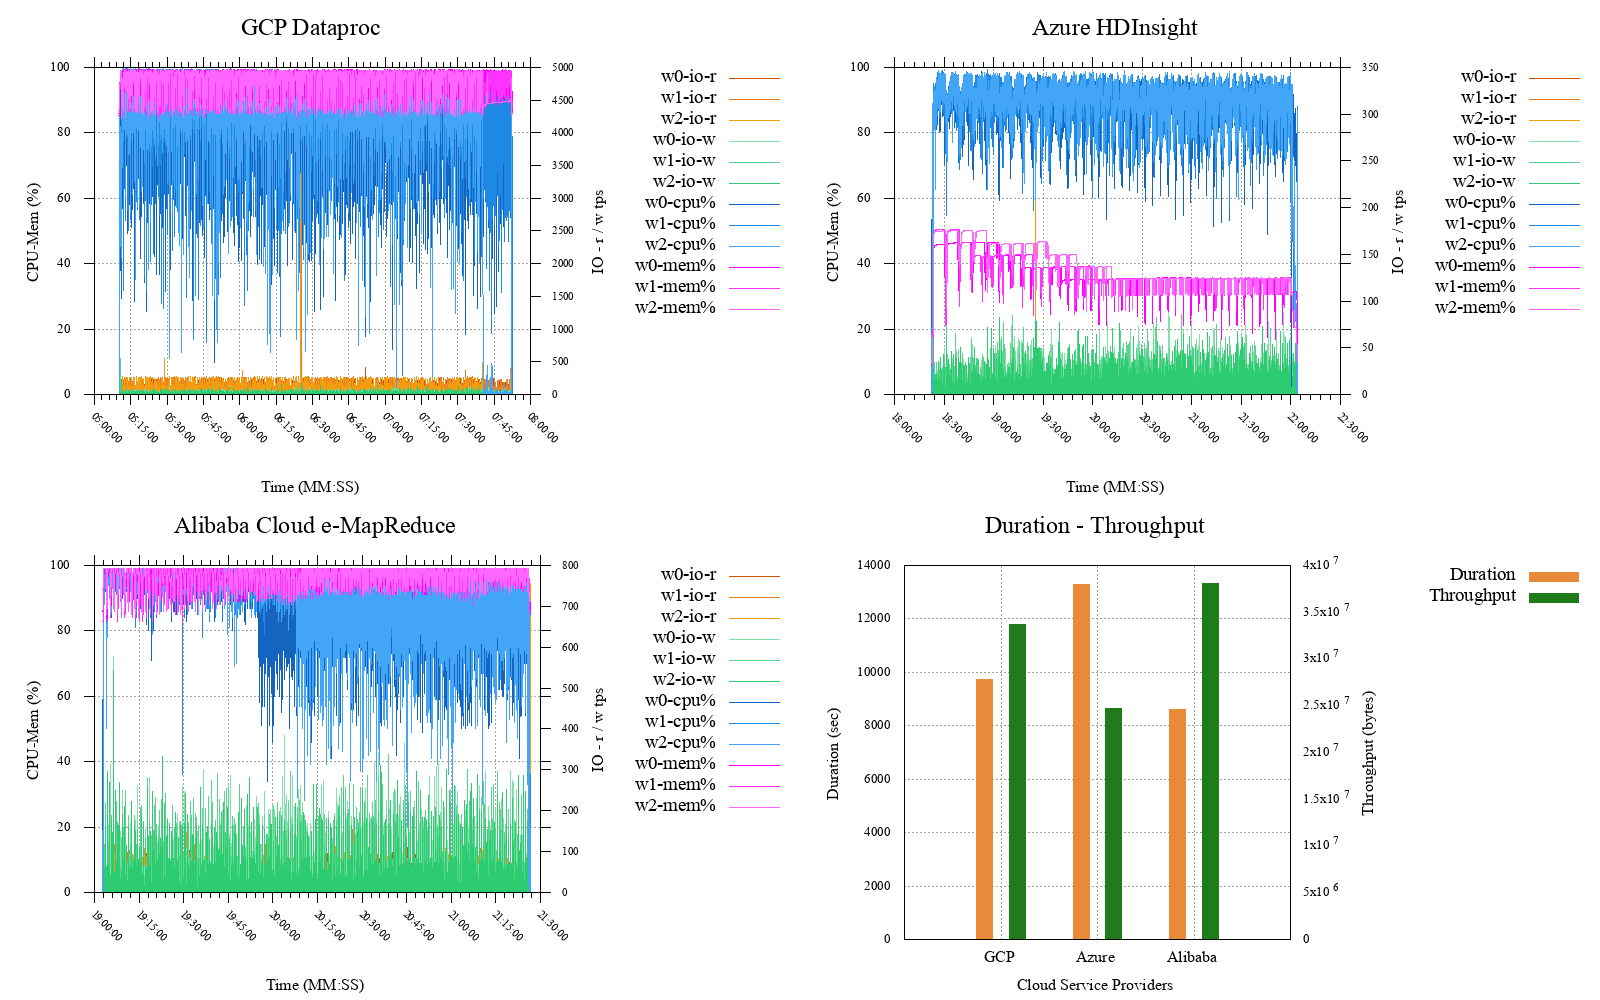
\includegraphics[width=\textwidth]{uc2-wrdcnt-g-cmidt}
	\centering
\end{figure}

%Serkan: Dicussion kısmını da biraz değiştirdim.
\section{Discussion}
Managed Hadoop systems are by CSPs provided cloud service proposals comprising pre-installed and pre-configured Hadoop clusters in order to eliminate the hard work on planning and installing Hadoop clusters manually on VM instances. As a result, they simplify the cluster installation to a matter of property selection and letting end-users focus only to applications that run on the cluster. As managed systems come in a black-box nature, respective pre-configurations and their impacts on the cluster performance remain unclear to the end-user. 

In the study, we attempted to bring more clarity to black-box nature of managed Hadoop services of major cloud providers by evaluating the performances of the services in terms of resource utilization using various benchmark tasks. To provide a fair comparative assessment, we utilized the managed services as they are given out-of-the-box by the cloud providers without applying any configurations to change their expected performances. 

One major limitation of the study has been the high-cost of benchmark executions' total running time charged in a pay-per-use manner, which led us to limit benchmark executions at only one successful execution for each workload. In future work, we plan on executing each benchmark three times and taking the average, which might have provided more stable outcomes, especially in cases, where there were small differences between subsequent performances of respective providers. 

Another result of the limitation mentioned above is that we also left off the largest predefined data scale of HiBench, namely Bigdata. This benchmark's execution would have provided performance outputs in a vast data scale, for instance, 300 GB for Sort, 1.6 TB for Wordcount, and 12.000.000 pages by 1.000.000.000 user visits for Aggregation. Hence, we do not recommend the study to be considered as a grading board for respective managed Hadoop systems' business values but it should be used as a guide for anticipating the performances of different platforms in various tasks when choosing cloud providers.

HiBench comes with dependencies downloaded during its compilation process by Apache Maven. The Hive engine is one of those dependencies leveraged by HiBench for running SQL workloads Scan, Join, and Aggregation. Alibaba's e-Mapreduce comprises a ready-made Hive hook triggering a Java file to run post-execution transactions for other services within the package. However, this configuration prevented HiBench from starting with respective benchmarks' execution since the HiBench based Hive engine does not include the jar file mentioned above defined for e-MapReduce's specific environment. 

A workaround attempt, copying the related jar file to an appropriate directory within HiBench, made the jar file available. However, this time, HiBench's Hive engine of an older version did not support the event     "hive.exec.post.hooks" defined in Alibaba's Hive configuration. At this point, disabling the respective Hive hook from Alibaba e-MapReduce's UI management console apparently solved this issue and enabled HiBench's SQL workloads to run, but its impact on the respective performance values remains unknown, hence the need to annotate it here. With GCP and Azure, issues of this kind did not occur.

%bu sayısal sonuçlar içeren metinler, figure ve tablolar discussion için uygun değil. Bir kısmını Results'a taşımak gerekiyor.
In the Azure environment, the Terasort benchmark running in data scale gigantic failed to complete in all three attempts we conducted where about 20\% of map operations were reached. Showing distinction to GCP and Alibaba where the end-user is liberated in choosing HDFS or the respective provider's cloud storage service as the cluster's file system, Azure obligates the user to go with WASB blob storage among other Azure storage services with a promise to Peta-scale. 

However, after inspecting the failure, it turned out that the exception is not due to the WASB. Even though WASB is predefined as the cluster's file system, during the application's run time, YARN still leverages the cluster's HDFS file system to store intermediate results and fail to allocate free space HDFS reaching specific levels of maps operators. We marked this failure as a structural bottleneck since all end users running Terasort operation at this scale would face the same error, and since resource utilization can be tracked up to the failure point and after, we kept this benchmark by marking it as incomplete. Figure \ref{fig:uc1-tera-g-cmidt} displays system resource utilization on Azure, including the point where the failure occurs.

Along with the resource utilization vs. performance plots both for Use Case 1 and Use Case 2, it is easily recognizable how likely structured architectures, namely GCP Dataproc and Alibaba Cloud e-MapReduce, both leveraging a rather conventional Hadoop installation and infrastructure, follow a similar pattern in utilization over time whereas a different architectural approach distinct in its performance behavior as in Azure's HDP based HDInsight. 

To better understand the relative performance dynamics, we gathered and processed the CSPs' HiBench performances in duration (seconds) in Table \ref{tab:uc1-comparative-results} and Table \ref{tab:uc2-comparative-results}. Column "Benchmark" refers to the respective benchmark executed, column "First" contains the best-performing provider, column "Second" points out the provider service with the second shortest duration, column "Third" lists the provider of the longest duration for the respective benchmark. The columns "-Perf\%" display the relatively low performance of the respective provider's service listed to their left with respect to the best performing service's value. \textit{Relative Performance Rate = (Shortest duration - Current duration) / Shortest duration}. 

Relative Performance Rates indicate that in overall, alike architectures are close in their results and competitive like performing the same duration in UC1-Aggregation or as close as 0.17\% time difference. The farthest distance between GCP and Alibaba is 65.97\% in UC2-Pagerank.

%%Use Case 1 Relative Performance Rates:
\begin{table}
	\centering
	\small
	\caption{Use Case 1 Relative Performance Rates}
	\label{tab:uc1-comparative-results}
	\begin{tabular}[h!]{ l l r r r r }
		\multicolumn{6}{ c }{Data Scale: Huge}  \\
		{Benchmark} & First & Second & -Perf.\% & Third & -Perf.\% \\
		\hline
		Sort & GCP & Alibaba & -58.57\% & Azure & -87.14\% \\
		Terasort & GCP & Azure & -28.64\% & Alibaba & -58.02\% \\
		Wordcount & Alibaba & GCP & -10.01\% & Azure & -65.35\% \\
		Dfsioe-r & Alibaba & GCP & -20.00\% & Azure & -170.20\% \\
		Dfsioe-w & Alibaba & GCP & -34.88\% & Azure & -134.16\% \\
		Scan & GCP & Alibaba & -1.37\% & Azure & -115.07\% \\
		Join & Alibaba & GCP & -3.43\% & Azure & -103.43\% \\
		Aggregation & GCP-Alibaba & --- & --- & Azure & -121.65\% \\
		Bayes & GCP & Alibaba & -15.86\% & Azure & -135.02\% \\
		Kmeans & Alibaba & Azure & -11.74\% & GCP & -12.13\% \\
		Pagerank & GCP & Alibaba & -59.20\% & Azure & -115.93\% \\
		\hline
		\multicolumn{6}{ c }{Data Scale: Gigantic}  \\
		{Benchmark} & First & Second & -Perf.\% & Third & -Perf.\% \\
		\hline
		Sort & GCP & Azure & -10.07\% & Alibaba & -25.31\% \\
		Terasort & Alibaba & GCP & -1.67\% & Azure & --- \\
		Wordcount & Alibaba & GCP & -16.84\% & Azure & -56.80\% \\
		Dfsioe-r & Alibaba & GCP & -38.64\% & Azure & -185.76\% \\
		Dfsioe-w & Alibaba & GCP & -27.08\% & Azure & -80.57\% \\
		Scan & Alibaba & GCP & -12.29\% & Azure & -26.29\% \\
		Join & Alibaba & GCP & -0.17\% & Azure & -28.11\% \\
		Aggregation & GCP & Alibaba & -8.03\% & Azure & -13.58\% \\
		Bayes & GCP & Alibaba & -18.93\% & Azure & -135.31\% \\
		Kmeans & Alibaba & Azure & -0.20\% & GCP & -12.57\% \\
		Pagerank & GCP & Azure & -40.71\% & Alibaba & -65.97\% \\
		\hline
	\end{tabular}
\end{table}



%%Use Case 2 Relative Performance Rates:
\begin{table}
	\centering
	\small
	\caption{Use Case 2 Relative Performance Rates}
	\label{tab:uc2-comparative-results}
	\begin{tabular}[h!]{ l l r r r r }
		{Benchmark} & First & Second & -Perf.\% & Third & -Perf.\% \\
		\hline
		Sort (t) & Alibaba & GCP & -12.50\% & Azure & -115.63\% \\
		Sort (s) & Alibaba & GCP & -16.13\% & Azure & -125.81\% \\
		Sort (l) & GCP-Alibaba & --- & --- & Azure & -92.86\% \\
		Sort (h) & GCP & Alibaba & -52.86\% & Azure & -101.43\% \\
		Sort (g) & GCP & Azure & -0.72\% & Alibaba & -27.23\% \\
		Wordcount (t) & Alibaba & GCP & -22.58\% & Azure & -119.35\% \\
		Wordcount (s) & Alibaba & GCP & -6.38\% & Azure & -108.51\% \\
		Wordcount (l) & Alibaba & GCP & -7.50\% & Azure & -124.17\% \\
		Wordcount (h) & Alibaba & GCP & -7.21\% & Azure & -67.45\% \\
		Wordcount (g) & Alibaba & GCP & -13.07\% & Azure & -54.09\% \\
		\hline
		\multicolumn{6}{ r }{(t): tiny, (s): small, (l): large, (h): huge, (g): gigantic} \\
		\hline
	\end{tabular}
\end{table}

On the other hand, the Relative Performance Rates in Table \ref{tab:uc1-comparative-results} and Table \ref{tab:uc2-comparative-results} depict numerous samples where Azure's performance falls back the best duration by more than 100\%, meaning that performing at least two times slower in the respective benchmarks. A possible reason for the -170.20\% and -134.16\% low performances in UC1's Dfsioe's and -185.76\% and -80.57\% low performances in UC2's Dfsioe's might be the replacement of the native Hadoop filesystem by Azure blob. HDI performances for SQL benchmarks (Scan, Join, and Aggregation) move between -103\% and -121\% in UC1, whereas in UC2, a better performance moving along -13\% and -28\% occurs. 

Another contradictory case for Azure is in its ML performances, especially in gigantic data scale where for Bayes it low performs at -135.31\% whereas for Kmeans it almost scores the best performance, getting the second place by a performance slightly less than -0.20\% with respect to the shortest duration. Why is it so? In our attempt to understand this situation, we delved into the execution plans, generated initially by Hadoop during execution and further captured and stored by HiBench inside the Reports folder. Table \ref{tab:uc1-sql-mr-allocs} and Table \ref{tab:uc2-mr-allocs} comprise the allocated map and reduce slots by their respective Hadoop cluster for the relevant benchmarks. It turns out that GCP and Alibaba Cloud's managed services show themselves more capable in resource allocation to respective applications, hence competitive to each other. 

Another instance of the relatively low-performance Azure's, for Bayes benchmark in Use Case 1, might point to a structural shortcoming where the execution logs point Java heap space errors, which cause the job to restart nine times, thus prolonging the overall duration of the benchmark, and resulting in termination at the end. Azure's default configurations somewhat lack to provide free resources enough to stay in the competition and this might be resolved with performance tuning, though. Having sufficient resources, Azure almost outperforms its conjugates in K-means, leveraging the very same Mahout engine with Bayes benchmark. Scoring its highest (-0.20\%) and lowest (-135.31\%) relative performances in the same category (ML) is somewhat contradictory but reasonable when considering the low performance as a structural pre-configuration issue.

%% Allocated maps and reduces in SQL benchmarks
\begin{table}
	\centering
	\small
	\caption{Allocated map and reduce slots in SQL benchmarks of Use Case 1}
	\label{tab:uc1-sql-mr-allocs}
	\begin{tabular}[h!]{ l r r r r r r l }
		{} & \multicolumn{2}{c}{GCP} & \multicolumn{2}{c}{Azure} & \multicolumn{2}{c}{Alibaba} & {} \\
		{Benchmark} & {Maps} & Reduces & {Maps} & Reduces & {Maps} & Reduces & Ref. \\
		\hline
		Scan * (h) & 24 & -- & 12 & -- & 24 & -- & {\textit{Fig.\ref{fig:uc1-scan-h-cmidt}}} \\
		Scan * (g) & 144 & -- & 36 & -- & 144 & -- & {\textit{Fig.\ref{fig:uc1-scan-g-cmidt}}} \\
		Join (h) & 60 & 25 & 48 & 25 & 60 & 25 & {\textit{Fig.\ref{fig:uc1-join-h-cmidt}}} \\
		Join (g) & 180 & 25 & 72 & 25 & 180 & 25 & {\textit{Fig.\ref{fig:uc1-join-g-cmidt}}} \\
		Aggregation (h) & 24 & 12 & 12 & 12 & 24 & 12 & {\textit{Fig.\ref{fig:uc1-aggreg-h-cmidt}}} \\
		Aggregation (g) & 144 & 12 & 36 & 12 & 144 & 12 & {\textit{Fig.\ref{fig:uc1-aggreg-g-cmidt}}} \\
		\hline
		\multicolumn{8}{ r }{(h): huge, (g): gigantic} \\
		\multicolumn{8}{ r }{* No reduce operation} \\
		\hline
	\end{tabular}
\end{table}

%% Allocated maps and reduces in Use Case 2
\begin{table}
	\centering
	\small
	\caption{Allocated map and reduce slots in Use Case 2}
	\label{tab:uc2-mr-allocs}
	\begin{tabular}[h!]{ l r r r r r r l }
		{} & \multicolumn{2}{c}{GCP} & \multicolumn{2}{c}{Azure} & \multicolumn{2}{c}{Alibaba} & {} \\
		{Benchmark} & {Maps} & Reduces & {Maps} & Reduces & {Maps} & Reduces & Ref. \\
		\hline
		Sort (t) & 11 & 12 & 12 & 12 & 11 & 12 & {\textit{Fig.\ref{fig:uc2-srt-t-cmidt}}} \\
		Sort (s) & 11 & 12 & 12 & 12 & 11 & 12 & {\textit{Fig.\ref{fig:uc2-srt-s-cmidt}}} \\
		Sort (l) & 12 & 11 & 12 & 12 & 11 & 11 & {\textit{Fig.\ref{fig:uc2-srt-l-cmidt}}} \\
		Sort (h) & 24 & 12 & 12 & 12 & 23 & 12 & {\textit{Fig.\ref{fig:uc2-srt-h-cmidt}}} \\
		Sort (g) & 251 & 12 & 60 & 12 & 252 & 12 & {\textit{Fig.\ref{fig:uc2-srt-g-cmidt}}} \\
		Wordcount (t) & 11 & 12 & 12 & 12 & 11 & 12 & {\textit{Fig.\ref{fig:uc2-wrdcnt-t-cmidt}}} \\
		Wordcount (s) & 12 & 11 & 12 & 12 & 12 & 11 & {\textit{Fig.\ref{fig:uc2-wrdcnt-s-cmidt}}} \\
		Wordcount (l) & 24 & 11 & 12 & 12 & 23 & 12 & {\textit{Fig.\ref{fig:uc2-wrdcnt-l-cmidt}}} \\
		Wordcount (h) & 250 & 11 & 60 & 12 & 252 & 12 & {\textit{Fig.\ref{fig:uc2-wrdcnt-h-cmidt}}} \\
		Wordcount (g) & 2447 & 12 & 612 & 12 & 2447 & 11 & {\textit{Fig.\ref{fig:uc2-wrdcnt-g-cmidt}}} \\
		\hline
		\multicolumn{8}{ r }{(h): huge, (g): gigantic} \\
		\hline
	\end{tabular}
\end{table}

%Serkan:Conclusion biraz uzun olmuş. Biraz kısalttım.
\section{Conclusion and Future Work}
In the study, we conducted HiBench benchmarks against Hadoop PaaS clusters in their proposed, out-of-the-box form, provided by respective CSPs. For each CSP, among the proposed installation specifications, we selected the same geographical location as the region and by promise apparently the same CPU and Memory properties. Our aim was to compare those systems' performance behaviors by leveraging HiBench Benchmark Suite. We executed Hadoop related benchmarks on all three Hadoop on PaaS services and captured system resource utilization data in the meanwhile. The line chart and spider plot visualizations leveraging aforementioned outputs spitted out high-resolution scans of respective executions over time and a comparison of cluster-based performance averages. 

Based on the performance results, we calculated relative performance rates for each CSP's managed system related to the best performing one to get a better view of how far the respective performances distinct from each other. In the final stage, for selected benchmark performances, we gathered the numbers of the allocated map and reduce slots by vendors' managed Hadoop systems. We found that there is a strong relation between sufficiently allocated map slots and the performance output; hence it appears that default pre-configuration settings somewhat do not let sufficient resources to utilize, resulting in low performance for a vendor.

The results yielded that Hadoop PaaS offerings by vendors' promise do not necessarily utilize system resources in similar ways hence may highly distinct in some cases. We assumed that CSP's pre-configuration choices impact performance results even with the same hardware settings. The end-users shall be aware of their use cases' requirements, truly understand the default configuration proposals and their respective outcome, and possess the know-how to improve respective vendors' default configurations. %Based on the gained experience, the study might be varied in an approach more sensitive in balancing small performance differences among CSPs. 
Future work will include further benchmarks of Spark, graph, and streaming offered by HiBench and expand the scope of performance comparison evaluations to additional cloud vendors. %Micro cases like benchmarking before and after configuration tweaks could be possible approaches to go.

%\section*{References}
\bibliography{mybibfile}

\end{document}